\documentclass[12pt]{report}
\usepackage[a4paper,top=2cm,bottom=3.5cm,left=2.2cm,right=2.2cm]{geometry}
\usepackage{fancyhdr}
\usepackage{float}
\usepackage[english]{babel}
\usepackage{amsmath}
\usepackage{graphicx}
\usepackage{subcaption}
\usepackage{hyperref}
\usepackage{algorithm}
\usepackage{cite}
\usepackage{multicol}
\usepackage[noend]{algpseudocode}
\setcounter{tocdepth}{2}
\usepackage{amsfonts}
\usepackage{longtable}
\usepackage{booktabs}
\usepackage{adjustbox}

\algnewcommand\algorithmicforeach{\textbf{for each}}
\algdef{S}[FOR]{ForEach}[1]{\algorithmicforeach\ #1\ \algorithmicdo}

\makeatletter
\def\BState{\State\hskip-\ALG@thistlm}
\makeatother

\begin{document}

\begin{titlepage}
	\begin{center}

  \begin{minipage}{\linewidth}
      \centering
      \begin{minipage}{0.2\linewidth}
          \begin{figure}[H]
              
\includegraphics[width=\linewidth]{media/uni.png}
                       \end{figure}
      \end{minipage}
      \hspace{0.05\linewidth}
      \begin{minipage}{0.3\linewidth}
          \begin{figure}[H]
              
\includegraphics[width=\linewidth]{media/dei.png}
                       \end{figure}
      \end{minipage}
  \end{minipage} \\
[14mm] 
\textsc{\Large{University of Padua}} \\
[4.5mm]
\textsc{\Large Master Degree in Computer Engineering} \\
[4.5mm]
\textsc{\large A.Y. 2019/2020}\\
[3.5cm]
\textsc{\Large Operations Research Course Report}\\
[1cm]
\textsc{\Huge \textbf{ \textsl{Travelling Salesman Problem}}}\\
[7.5cm]
\textsc{\Large \textit{ \textsl{Barison Marco}}}\\
[0.4cm]
\textsc{\Large \textit{ \textsl{Moratello Matteo}}}\\
[0.4cm]
\textsc{\Large \textit{ \textsl{Obetti Christian}}}\\

	\end{center} 

\end{titlepage}

\newgeometry{top=3.5cm,bottom=3.5cm,left=3cm,right=3cm}

\begin{abstract}
On this report we present the traveling salesman problem (TSP), an optimization problem where we want to find the best Hamiltonian path on a given graph, and some deterministic and heuristic solutions to resolve it. The goal of our work is to implement some of the most known algorithms in the literature of the operational research and analyze them to discover which are the best ones to resolve this particular optimization problem.
Each solution is tested on a dataset of different instances, results are then compared using a performance profile. \\
The first part of the report is focused on algorithm based on CPLEX, the solver that we used for this research. These are mostly deterministic algorithms, so they work well only with relatively small instances (less than 600-700 nodes). After realizing the performance profile we can conclude that the best deterministic algorithm is the one based on generic callbacks plus user cut.\\
In the second part of the report we analyze generic heuristic solutions (so not based on CPLEX), ideal to resolve very big instances. After our tests we conclude that VNS (variable neighborhood search) is a very good algorithm for the TSP, simulated annealing can also be a valid alternative while the genetic algorithm has very poor performance.

\end{abstract}




\tableofcontents

\pagestyle{fancy}
\renewcommand{\sectionmark}[1]{\markboth{\thesection.\ #1}{}}
\fancyhead[L]{\nouppercase{Operations Research 2}}
\fancyhead[R]{\nouppercase{Barison, Moratello, Obetti}}


\chapter{Introduction}

Qui un intro sul problema TSP direi

\chapter{Compact Models}
Here we introduce different formulations for the traveling salesman problem that we implemented. For all the following models we will use the decision variable $x_{ij}$ already defined in Section \ref{TSPdef}.\\
According to \cite{ormanWilliams}, we considered the case of the Asymmetric version of the traveling salesman problem, which can be considered more general than the Symmetric version.\\
Main advantage of going with these models, is that once the model is written, it can be solved as a ``black box" by CPLEX solver.\\
To improve the time performance in the computation of the optimal solution, we implemented part of constraints about the subtour elimination through \textit{lazy constraints}. This allowed us to improve the performance of the models because this kind of constraints will be applied only once needed.

\section{Sequential formulation}
For this version, formulated by Miller, Tucker and Zemlin (MTZ) in 1960 \cite{MTZ}, we introduce the continuous variable 
\begin{equation*}
	u_i = \text{sequence in which point i is visited} \ (i \neq 1)
\end{equation*}
and the constraint \ref{eqn:mtz-constraint}.

\begin{subequations}
	\begin{equation}
		\text{min} \underbrace{\sum_{(i,j) \in A} c_{ij}x_{ij}}_\text{circuit cost}
	\end{equation}
	\begin{equation}
		\underbrace{\sum_{(i,j) \in \delta^{-}(j)} x_{ij} = 1}_\text{one edge incoming in j}, \quad j \in V 
		\label{eqn:2.1b}
	\end{equation}
	\begin{equation}
		\underbrace{\sum_{(i,j) \in \delta^{+}(j)} x_{ij} = 1}_\text{one edge outgoing in i}, \quad i \in V
		\label{eqn:2.1c}
	\end{equation}
	\begin{equation}
		u_i-u_j+nx_{ij} \leq n-1 \quad \forall i,j \in N-\lbrace 1 \rbrace, \ i\neq j \;\; \textbf{(Lazy constraint)}
		\label{eqn:mtz-constraint}
	\end{equation}
\end{subequations}

\noindent Constraints \ref{eqn:mtz-constraint} ensure that, if the salesman travels from i to j, then the position of node j is one more than that of node i. This allows to have only a polynomial number of variable and constraints. In total, there are $O(n^2)$ variables and $O(n^2)$ constraints. The problem is no more NP-Hard, but the relaxation of the problem is somewhat weak and as one can see in the section where compact models are compared, it yields to decent performances only for small instances.

\section{Flow-based formulations}

\subsection{Single commodity flow}
Provided by Gavish and Graves in 1978, it adds continuous variables: 
\begin{equation*}
	y_{ij} = \text{flow in arch} \ (i,j) \ i \neq j
\end{equation*}
%In total it has $n(n+2)$ constraints, $n(n-1)$ 0-1 variables and $n(n-1)$ continuous variables.

\begin{subequations}
	\begin{equation}
		\text{min} \sum_{(i,j) \in A} c_{ij}x_{ij} \\
	\end{equation}
	\begin{equation}
		\sum_{(i,j) \in \delta^{-}(j)} x_{ij} = 1, \quad j \in V \\
	\end{equation}
	\begin{equation}
		\sum_{(i,j) \in \delta^{+}(j)} x_{ij} = 1, \quad i \in V \\
	\end{equation}
	\begin{equation}
		y_{ij} \leq (n-1)x_{ij} \quad \forall i,j \in N, \ i \neq j \\
	\end{equation}
	\begin{equation}
		\sum_{j, \; j \neq 1} y_{1j} = n-1 \;\; \textbf{(Lazy constraint)}\\
	\end{equation}
	\begin{equation}
		\sum_{i, \; i \neq j} y_{ij} - \sum_{k, \; i \neq k} y_{jk} = 1 \quad \forall j \in N - \lbrace 1 \rbrace
	\end{equation}
\end{subequations}

\noindent The idea is that whenever one node is chosen, the salesman delivers one unit of commodity flow. In this way, an order between the nodes is picked and subtours are impossible.\\
This formulation has $O(n^2)$ variables and $O(n)$ constraints. The relaxation of the linear problem works better than the MTZ, as one can observe in the section about the comparison between the compact models.

\subsection{Two commodity flow}
Created by Finke, Claus and Gunn in 1983. It maintains constraint \ref{eqn:2.1b} and \ref{eqn:2.1c} (from this point they and the objective function will not be shown in the formulation) and introduce the continuous variables:
\begin{equation*}
	y_{ij} = \text{flow of commodity 1 in arc} \ (i,j) \ i \neq j
\end{equation*}
\begin{equation*}
	z_{ij} = \text{flow of commodity 2 in arc} \ (i,j) \ i \neq j
\end{equation*}
and add the constraints:

\begin{subequations}
	\begin{equation}
	\label{eqn:f2-const-1}
	 	\sum_{j, \; j \neq 1} (y_{1j}-y_{j1}) = n-1 \;\; \textbf{(Lazy constraint)}
	\end{equation}
	\begin{equation}
	\label{eqn:f2-const-2}
		\sum_{j} (y_{ij}-y_{ji}) = 1 \quad \forall i \in N-\lbrace 1 \rbrace, \ i \neq j
	\end{equation}
	\begin{equation}
	\label{eqn:f2-const-3}
		\sum_{j, \; j \neq 1} (z_{1j}-z_{j1}) = -(n-1) \;\; \textbf{(Lazy constraint)}
	\end{equation}
	\begin{equation}
	\label{eqn:f2-const-4}
		\sum_{j} (z_{ij}-z_{ji}) = -1 \quad \forall i \in N-\lbrace 1 \rbrace, \ i \neq j
	\end{equation}
	\begin{equation}
	\label{eqn:f2-const-5}
		\sum_{j} (y_{ij}+z_{ij}) = n-1 \quad \forall i \in N
	\end{equation}
	\begin{equation}
	\label{eqn:f2-const-6}
		y_{ij}+z_{ij} = (n-1)x_{ij} \quad \forall i, j \in N
	\end{equation}
\end{subequations}

%In total it has $n(n+4)$ constraints, $n(n-1)$ 0-1 variables and $2n(n-1)$.
\noindent Constraints \ref{eqn:f2-const-1} and \ref{eqn:f2-const-2} force $(n-1)$ units of commodity 1 to flow into city 1 and 1 unit of commodity to flow out from every other node.\\
Constraits \ref{eqn:f2-const-3} and \ref{eqn:f2-const-4} force $(n-1)$ units of commodity 2 to flow out from city 1 and 1 unit of commodity to flow into every other node.\\
Constraints \ref{eqn:f2-const-5} force exactly $(n-1)$ units of commodity in each arc and constraints \ref{eqn:f2-const-6} only allow flow in an arc if present.\\
The formulation has $O(n^2)$ constraints and $O(n^2)$ variables.

\subsection{Multi-commodity flow}
Proposed by Wong and Claus in 1984. Again constraint \ref{eqn:2.1b} and \ref{eqn:2.1c} are maintained. It introduce the continuous variable:
\begin{equation*}
	y_{ij}^k = \text{flow of commodity k in arc} \ (i,j) \in N-\lbrace 1 \rbrace
\end{equation*}
and the following constraints:
\begin{subequations}
	\begin{equation}
	\label{eqn:fm-const-1}
		y_{ij} \leq x_{ij} \quad \forall i,j,k \in N, \ k \neq 1
	\end{equation}
	\begin{equation}
	\label{eqn:fm-const-2}
		\sum_{i} y_{1i}^k = 1 \quad \forall k \in N-\lbrace 1 \rbrace
	\end{equation}
	\begin{equation}
	\label{eqn:fm-const-3}
		\sum_{i} y_{i1}^k = 0 \quad \forall k \in N-\lbrace 1 \rbrace
	\end{equation}
	\begin{equation}
	\label{eqn:fm-const-4}
		\sum_{i} y_{ik}^k = 1 \quad \forall k \in N-\lbrace 1 \rbrace
	\end{equation}
	\begin{equation}
	\label{eqn:fm-const-5}
		\sum_{j} y_{kj}^k = 0 \quad \forall k \in N-\lbrace 1 \rbrace
	\end{equation}
	\begin{equation}
	\label{eqn:fm-const-6}
		\sum_{i} y_{ij}^k - \sum_{i} y_{ji}^k = 0 \quad \forall j,k \in N-\lbrace 1 \rbrace, \ j \neq k
	\end{equation}
\end{subequations}
%In total there are $n^3+n^2+6n-3$ constraints, $n(n-1)$ 0-1 variables and $n(n-1)^2$
Constraints \ref{eqn:fm-const-1} only allow flow in an arc which is present. Constraints \ref{eqn:fm-const-2} force exactly one unit of each commodity to flow into city 1 and constraints \ref{eqn:fm-const-3} does the opposite, preventing commodity to flow out from city 1.\\
Constraints \ref{eqn:fm-const-4} force exactly one unity of commodity k to flow out from city k and constraints \ref{eqn:fm-const-5} prevent any of commodity k flowing into city k.\\
Finally, constraints \ref{eqn:fm-const-6} force balance for all commodities at each node, apart from city 1 and for commodity k at city k.\\
There is a total number of $O(n^3)$ constraints and $O(n^2)$ variables.

\section{Time staged formulations}

We decided also to explore this section of compact models, exploiting CPLEX's solver that just requires the models to be written. Dealing with performance, especially the T1 and T2 were not working good in practice and required too much to compute the optimal solution.

\subsection{First stage dependent}
Introduced by Fox, Gavish and Graves in 1980. Constraint \ref{eqn:2.1b} and \ref{eqn:2.1c} are maintained, in addition we have 0-1 integer variables:
\[ y_{ij}^t =
	\begin{cases}
		1 \quad \text{if the edge} \ (i,j) \ \text{is traversed at stage t} \\
		0 \quad \text{otherwise}
	\end{cases}
\]
and constraints below, for a total of $n(n+2)$ constraints and $n(n-1)(n+1)$ 0-1 variables.

\begin{subequations}
	\begin{equation}
		\sum_{i,j,t} y_{ij}^t = n
	\end{equation}
	\begin{equation}
		\sum_{j,t \; t \geq 2} ty_{ij}^t - \sum_{k,t} ty_{ki}^t = 1 \quad \forall i \in N-\lbrace 1 \rbrace 
	\end{equation}
	\begin{equation}
		x_{ij}-\sum_{t} x_{ij}^t = 0 \quad \forall i,j \in N, \ i \neq j
	\end{equation}
	with the condition
	\begin{equation}
		y_{il}^t = 0 \; \forall t \neq n, \quad y_{ij}^t = 0 \; \forall t \neq 1, \quad y_{ij}^l = 0 \; \forall i \neq 1, \quad i \neq j
	\end{equation}
\end{subequations}

\subsection{Second stage dependent}
Provided by Fox, Gavish and Graves in 1980. It uses the same variables of first stage and constraints \ref{eqn:2.1b} and \ref{eqn:2.1c} and it adds:

\begin{subequations} 
	\begin{equation}
		\sum_{i,t \; i \neq j} y_{ij}^t = 1 \quad \forall j \in N
	\end{equation}
	\begin{equation}
		\sum_{j,t \; j \neq i} y_{ij}^t = 1 \quad \forall i \in N
	\end{equation}
	\begin{equation}
		\sum_{i \; j \neq i} y_{ij}^t = 1 \quad \forall t \in N
	\end{equation}
	\begin{equation}
		\sum_{j,t \; t \geq 2} ty_{ij}^t - \sum_{k,t} ty_{ki}^t = 1 \quad \forall i \in N-\lbrace 1 \rbrace \;\; \textbf{(Lazy constraint)}
	\end{equation}
\end{subequations}
In totals there are $4n-1$ constraints and $n(n-1)(n+1)$ 0-1 variables.

\subsection{Third stage dependent}
Again we have the same variables of first stage and constraints \ref{eqn:2.1b} and \ref{eqn:2.1c}. In addition, 
for a total of $2n^2-n+3$ constraints and $n(n-1)(n+1)$ 0-1 variables we have:
\begin{subequations}
	\begin{equation}
		\sum_{j} y_{1j}^1 = 1
	\end{equation}
	\begin{equation}
		\sum_{i} y_{i1}^n = 1
	\end{equation}
	\begin{equation}
		\sum_{j} y_{ij}^t - \sum_{k} y_{ki}^{t-1} = 0 \quad \forall i,t \in N-\lbrace 1 \rbrace
	\end{equation}
\end{subequations}
\newpage
\section{Final comparison between Compact Models}
As explained in the previous sections, we decided mainly to focus on MTZ and Flow Based formulations, because of the time required to compute the optimal solution for the dataset we used.\\
We tested these algorithms on dataset made of instances with a number of nodes up to 80. For bigger instances, the computation of an optimal solution became unfeasible.\\
The instances we used to test all our implementations, from compact models to heuristic algorithms, are taken from the TSPLIB \cite{tsplib}. \\
From our results shown in Figure \ref{fig:compacts10} and \ref{fig:compacts200}, we observed that FLOW1 outperformed the other algorithms. Decent results were obtained also with MTZ and FLOW2. In our implementation, FLOW3 had poor performances.

\begin{figure}[H]
\centering
	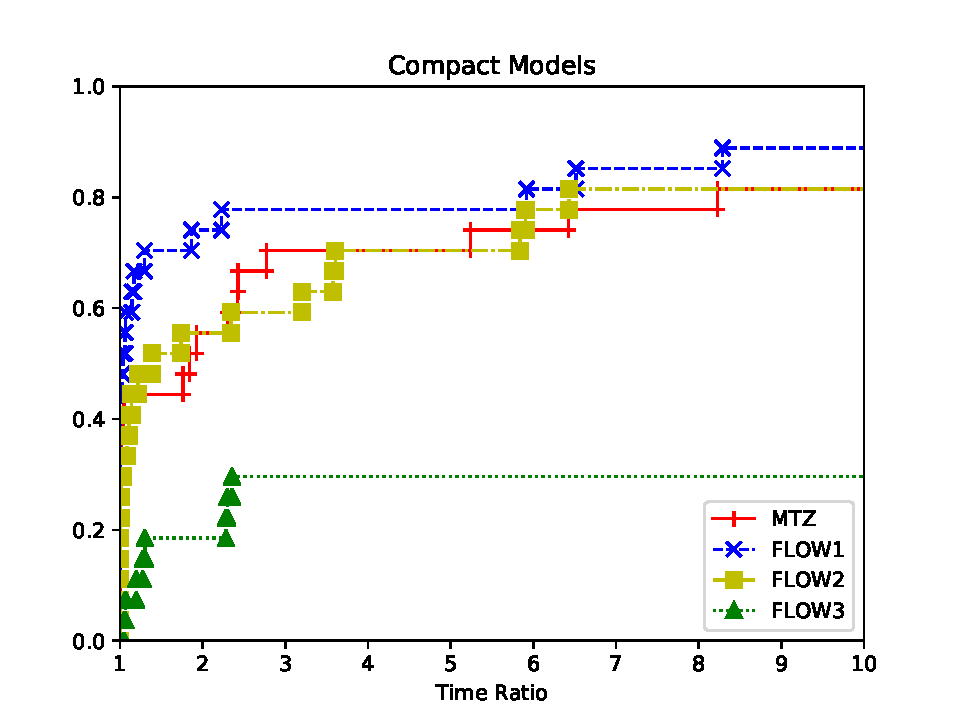
\includegraphics[scale=0.9]{media/compact10.pdf} \\
	\caption{Performance profile for compact models with time ratio 10}
	\label{fig:compacts10}
\end{figure}

\begin{figure}[H]
\centering
	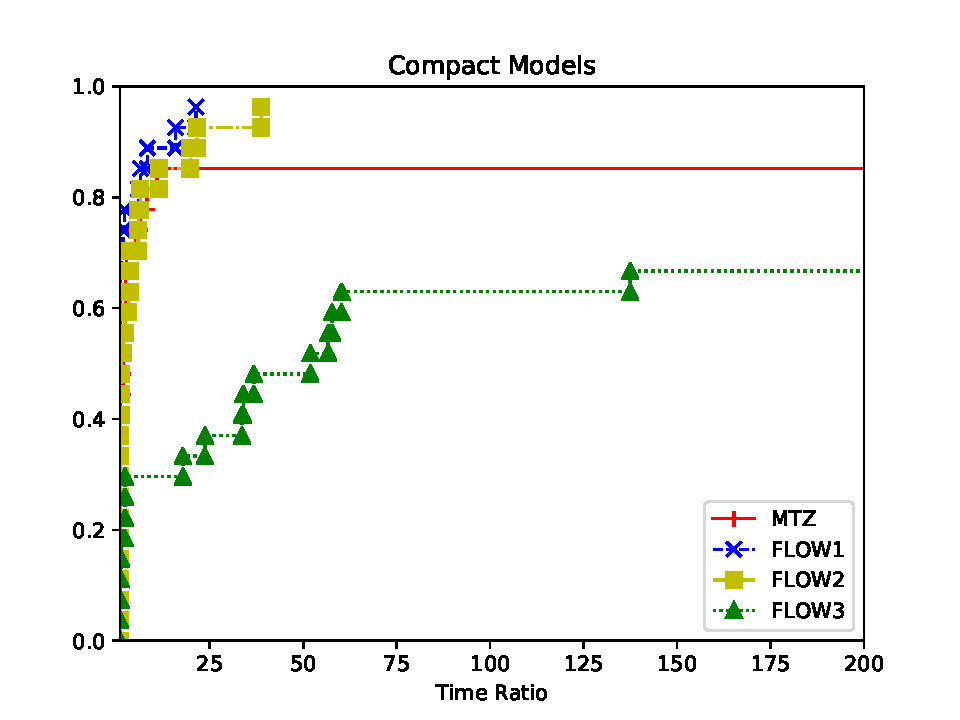
\includegraphics[scale=0.9]{media/compact200.pdf} \\
	\caption{Performance profile for compact models with time ratio 200}
	\label{fig:compacts200}
\end{figure}





\chapter{Exact Algorithms}

In this chapter we will describe exact algorithms based on the Symmetric version of the Dantzig-Fulkerson-Johnson formulation \cite{DFJ}. The main problem of this model is that the formulation has $O(2^n)$ SECs, so it is impossible to implement all the constraints in the model since it would result in a very high execution time and memory usage even for small graphs.
\\ For this reason, SECs are added only when necessary to the model, in order to discard solutions with cycles. Using this technique, hopefully, only a small fraction of the $O(2^n)$ SECs will be added to the model.
\\ The main algorithms that make use of this technique to solve TSP instances to optimum (of even considerable size) are Loop Methods and CPLEX Callbacks.

\section{Loop Methods}
On this section we will describe two iterative approaches, originally proposed by \cite{bender}, in order to solve the DFJ model without adding an exponential number of Cycle constraints.
\subsection{Simple Loop}
The first approach, that we called Simple Loop, is presented in Algorithm \ref{alg:simpleloop}.
\\ In line 2, we initialize the model with the variables, the degree constraints and the objective function. 
The algorithm then proceeds solving the problem within a while loop (lines 3-4), and at each iteration we check if the optimal solution has more than one component (line 5). If so, we add, for each component, the corresponding subtour eliminator (line 6). \\Instead, if the optimal solution has one component (lines 7-8), that is, it is a Hamiltonian cycle, then we return the optimal solution found (line 9).
\\ This algorithm turns out very efficient, especially with recent solvers. Its efficiency is due to the fact that the solution is solved very fast, especially in first iterations, and only small number of SECs are added at each iteration. These constraints allow to exclude a lot of solutions with subtours of the original problem. 
\\ At worst, since the problem is NP-hard, all constraints will be added to the model, requiring exponential computational time, but in most cases this doesn't happen.
It may seem that this method is not very efficient, but with recent and increasingly sophisticated solvers, it can lead to the optimal solution, even with many nodes, in few seconds.
\begin{algorithm}
    \caption{Simple Loop}\label{Loop Method}
    \hspace*{\algorithmicindent} \textbf{Input:} $G = (V,E) , \; c : E \rightarrow \mathbb{R}^+$\\
    \hspace*{\algorithmicindent} \textbf{Output:} $\textbf{\textit{z}\text{*}} $ optimal solution to TSP on the input graph $G$
    \begin{algorithmic}[1]
    \State $\textit{done} \gets \textit{false}$
    \State model $ \leftarrow $ \textbf{$\ast$ Initialize variables and objective function $\ast$ }
    \While {!done} 
    	\State $\textbf{\textit{z}\text{*}} \gets \text{optimal\_solution}(\text{model})$\;
	\If{$components(z\text{*}) > 1$} 
	\State \textbf{ $\ast$ Add SECs for each connected component to the model $\ast$ }
	
	\Else \State $\textit{done} \gets \textit{true}$
	\EndIf	
    \EndWhile
    \State \textbf{return} $\textbf{\textit{z}\text{*}} $
    \end{algorithmic}
    \label{alg:simpleloop}
    \end{algorithm}
\noindent
\subsection{Heuristic Loop}
The Algorithm \ref{alg:simpleloop} has a drawback since at each iteration we solve to optimum the TSP problem, even if the constraints collected until that point are not sufficient to achieve the true optimum. In other words, we must wait that the solver finds out the optimal solution, even if the constraints available may allow solutions with subtours.
\\ For this reason, we implemented an ``heuristic" version of the method seen before. This method is composed of two phases. The first phase is used to collect some SECs by relaxing the optimality concept, for example by setting an higher value for the solution GAP or limiting the solution in the root node of the branching tree.
This phase permits to add useful constraints to the model, without computing the optimal solution in each iteration. In fact, with this phase we can obtain a lot of useful SECs in a short time, especially in the first iterations.
This phase remains active until the solution found has more than one component, from then on, it will be activated the second phase. 
In the second phase, the solver's concept of ``relaxation" is removed and it essentially solve the problem with the Simple Loop method, ensuring that the solution returned is the true optimal solution.
\\ The Heuristic Loop is presented in Algorithm \ref{alg:heuloop}. In line 4, as in the first method, we initialize the model with the variables, the degree constraints and the objective function.
At the beginning, the first phase is active (line 2), which means that some CPLEX parameters have to be set (line 5) in order to obtain a non-optimal solution, thus speeding up the computational time. In our case, we decided to set three CPLEX parameters, that is, the MIP gap tolerance, the MIP node limit and the MIP solution limit. The first parameter force CPLEX to stop, when the solution found until that point has a GAP of a certain value (for example 5\%). The second parameter specifies the node of the branching tree until which CPLEX can compute the solution, for example, if the value of the parameter is set to 0, CPLEX can compute the solution only in the root node. The third parameter specifies the maximum number of integer solutions that the solver can compute. \\
The algorithm then proceeds solving the problem within a while loop (line 6). As in the Simple Loop, at each iteration we check if the solution has more than one component, and if so, we add, for each component, the corresponding SEC. \\ Instead, if the optimal solution has one component, we set the flag \textit{second\_phase} to true (line 15) and reset the solver settings, thus ensuring that the solution found from now on it will be an optimal solution.
During the first phase, we have hopefully collected a number of useful SECs in a small amount of time, compared to finding the optimal solution at each iteration.
For the description of the second phase please refer to the Simple Loop (Algorithm \ref{alg:simpleloop}).
\begin{algorithm}
    \caption{Heuristic Loop}\label{Loop Method}
    \hspace*{\algorithmicindent} \textbf{Input:} $G = (V,E) , \; c : E \rightarrow \mathbb{R}^+$\\
    \hspace*{\algorithmicindent} \textbf{Output:} $\textbf{\textit{z}\text{*}} $ optimal solution to TSP on the input graph $G$
    \begin{algorithmic}[1]
    \State $\textit{done} \gets \textit{false}$
    \State $\textit{first\_phase} \gets \textit{true}$
    \State $\textit{second\_phase} \gets \textit{false}$
    \State model $ \leftarrow $ \textbf{$\ast$ Initialize variables and objective function $\ast$ }
    \State CPXsetintparam $ \leftarrow $ \textbf{$\ast$ Set MIP gap tolerance, MIP node limit and MIP solution limit in order to obtain a non-optimal solution $\ast$ }
    \While {!done} 
    	\If{$second\_phase$} 
	\State CPXsetintparam $ \leftarrow $\textbf{ $\ast$ Return to original solver settings in order to obtain an optimal solution $\ast$ }
	\State $\textit{second\_phase} \gets \textit{false}$
	\EndIf
    	\State $\textbf{\textit{z}\text{*}}  \gets \text{optimal\_solution}(\text{model})$\;
	\If{$components(z\text{*}) > 1$} 
	\State \textbf{ $\ast$ Add SECs for each connected component to the model $\ast$ }
	\EndIf
	\If{$ components(z\text{*}) == 1 \And first\_phase$} 
	\State $\textit{first\_phase} \gets \textit{false}$
	\State $\textit{second\_phase} \gets \textit{true}$
	\EndIf
	\If{$ components(z\text{*}) == 1 \And !first\_phase$} 
	\State $\textit{done} \gets \textit{true}$
	\EndIf
    \EndWhile
    \State \textbf{return} $\textbf{\textit{z}\text{*}} $
    \end{algorithmic}
    \label{alg:heuloop}
    \end{algorithm}
    
\newpage
\subsection{Final comparison between Loop Methods}
\label{LMcomparision}
The dataset used to compare exact algorithms consists of 30 instances with four different random seeds \{201909284, 19, 190696, 19061996\}, for a total of 120 runs per algorithm. The instances used are the following:
 \begin{multicols}{3}
    \begin{itemize}
        \item a280.tsp
        \item att48.tsp
        \item att532.tsp
        \item berlin52.tsp
        \item bier127.tsp
        \item ch130.tsp
        \item ch150.tsp
        \item d198.tsp
        \item gil262.tsp
        \item kroA100.tsp
        \item kroA150.tsp
        \item kroA200.tsp
        \item kroB100.tsp 
        \item kroB150.tsp
        \item kroB200.tsp
        \item kroC100.tsp
        \item kroD100.tsp
        \item kroE100.tsp 
        \item lin105.tsp
        \item lin318.tsp 
        \item pr226.tsp 
        \item rat195.tsp 
        \item pr76.tsp 
        \item pr107.tsp 
        \item pr124.tsp
        \item pr136.tsp
        \item tsp225.tsp
        \item u159.tsp
        \item rat99.tsp
        \item rd400.tsp
    \end{itemize}
    \end{multicols}
\noindent
For each problem, we compare the elapsed time to compute the optimal solution.\\
In Figure \ref{fig:loops} it is possible to see the performance profile of the Loop Methods analyzed in this section.
The parameter we used are the following:
\begin{itemize}
 	\item \textbf{Simple Loop:} no parameters;
	\item \textbf{Heuristic Loop:} 
	\begin{itemize} 
		\item \textbf{MIP gap tolerance:} Absolute tolerance on the gap between the best integer objective and the objective of the best node remaining. Value used: 0.05;
		\item \textbf{MIP node limit:} Maximum number of nodes solved before the algorithm terminates. Value used: 0 (only the root node);
		\item \textbf{MIP solution limit:} Number of MIP solutions to be found before stopping. Value used: 1.
		\end{itemize}
\end{itemize}
The parameters for the Heuristic Loop are used in the first phase of the algorithm, then they are reset to their original values to find the optimal solution.
From the graphs we can see that the performance of the two algorithms are very similar. In the first phase of the Heuristic Loop, the SECs found are probably not sufficient to save time during the second phase of the algorithm. In our opinion, there is no reason to use the Heuristic Loop since, even with three parameters, there is always the risk to overtune the parameters using only few instances.

\begin{figure}[h!]
  \centering
  \begin{subfigure}[b]{0.97\linewidth}
    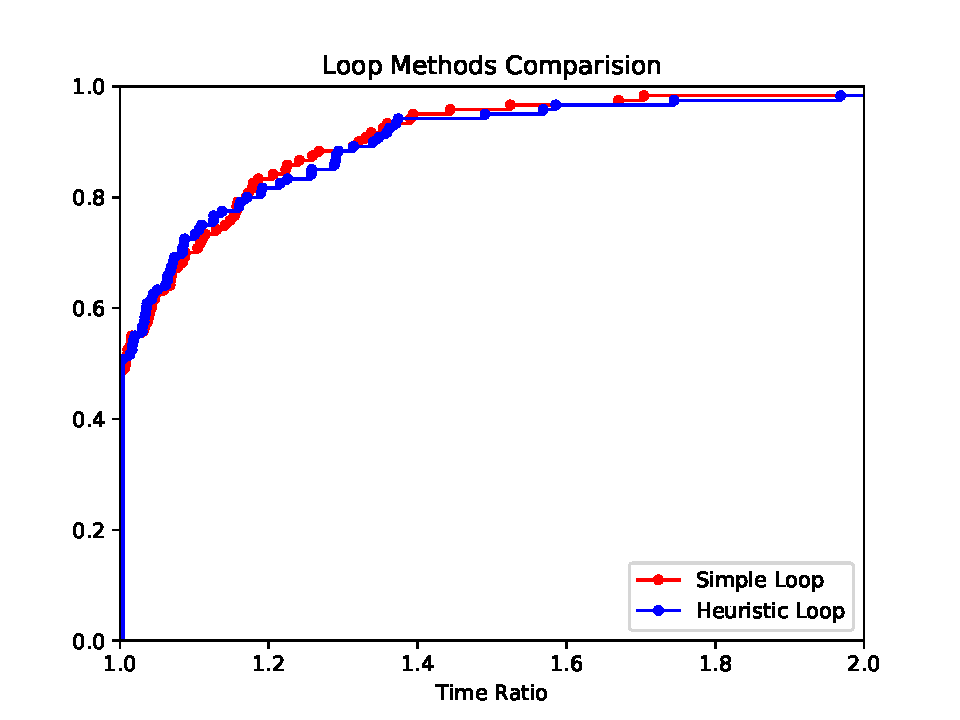
\includegraphics[width=\linewidth]{media/LoopMethods1.pdf}
  \end{subfigure}
  \begin{subfigure}[b]{0.97\linewidth}
    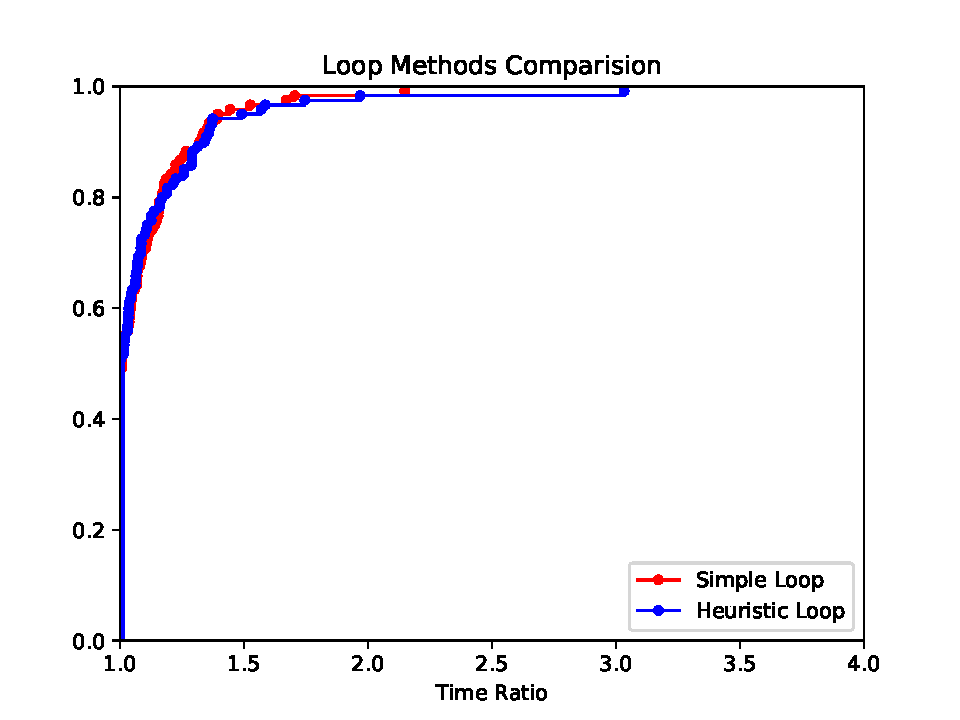
\includegraphics[width=\linewidth]{media/LoopMethods.pdf}
  \end{subfigure}
  \caption{On top: detailed view of the performance profile of Loop Methods. \\On the bottom: full view of the performance profile of Loop Methods.}
  \label{fig:loops}
\end{figure}

\clearpage
\section{Callbacks}
In this section we will describe how to solve the DFJ model using CPLEX callbacks. Until now, the algorithms we described resolve TSP instances with an iterative approach, that is, they solve multiple times a ``relaxed" model, adding the SECs when the solution found is composed of multiple tours. Since CPLEX uses the branch-and-cut technique to solve the MIP model, with the previous approach multiple decision trees will be created from scratch, losing much of the information from previous trees. Another way to handle the SECs is to exploit the branch-and-cut technique. In particular, when an integer solution is found by the solver during the decision tree, we can reject it if contains multiple tours by adding a SEC for each of them. With this method we develop only a single decision tree, and this results, hopefully, in a faster computation. To reach this goal, CPLEX provides a series of callbacks that can be used for adding constraints and solutions on the fly.

\subsection{Lazy Callback}
The lazy callback allows to resolve the TSP in a very fast and natural way. As described previously, in order to solve the problem we must reject solutions that have multiple tours, adding SECs on the fly. This leads to Algorithm \ref{alg:lazycall} in which we instantiate the model and the objective function as usual (line 2). Then we instantiate a procedure called LazyCallback (line 3). A LazyCallback is a function called by the solver when an integer solution is found during the branch-and-cut algorithm. The task of the callback is to check if the solution found has more than one connected component (line 8) and if it is the case, to reject the solution by adding the SECs to the model (lines 9 - 10). After this, the resolution of the model resumes (line 11).
The routine continues by optimally solving the model and returning the solution found (lines 4 - 5).


\begin{algorithm}
    \caption{Lazy Callback}\label{Lazy Callback}
    \hspace*{\algorithmicindent} \textbf{Output:} $\textbf{\textit{z}\text{*}} $ optimal solution to TSP on the input graph $G$
    \begin{algorithmic}[1]
   \Function{TSPopt}{$G = (V,E) , \; c : E \rightarrow \mathbb{R}^+$}
  \State model $ \leftarrow $ \textbf{$\ast$ Initialize variables and objective function $\ast$ }
  \State optimizer $ \leftarrow $ \textbf{$\ast$ Initialize the LazyCallback function within the optimizer $\ast$ }
  \State $\textbf{\textit{z}\text{*}} \gets \text{optimizer(model)}$
  \State \Return \textbf{\textit{z}\text{*}}
\EndFunction
\\
  \Function{LazyCallback}{\textbf{\textit{x}}, model}
  \State comp $ \leftarrow $ \textbf{$\ast$ number of components in the integer solution \textit{x} $\ast$ }
  \If{$ (comp > 1) $} 
	\State \textbf{ $\ast$ Add SECs for each connected component to the model $\ast$ }
	\EndIf  
	\State \Return 
	\EndFunction

    \end{algorithmic}
     \label{alg:lazycall}
    \end{algorithm}

\subsection{UserCut Callback}
Another interesting callback is the UserCut which is used to generate SECs on fractional solutions. The idea is pretty the same as the Lazy callback; when a fractional solution is found during the exploration of the decision tree by the solver, the UserCutCallback function checks the solution and adds constraints to the model on the fly. The procedure is described in algorithm \ref{alg:usercutcall}. In this case both LazyCallback and UserCutCallback must be defined (line 3). In particular, the UserCutCallback function checks how many components there are in the solution (line 14), if there are many connected components then it adds the SECs for each connected component (lines 15 - 16). Instead, when the graph is connected, we apply to the model the violated cuts, looking for sections with a capacity less than a certain threshold. The cutoff value is set to 2.0 - $\epsilon$, with $\epsilon$ = 0.1 in our implementation (lines 17 - 18). We used the \textit{Concorde}\footnote{\url{http://www.math.uwaterloo.ca/tsp/concorde.html}} algorithms in order to fast computing the connected components and violated cuts in fractional solutions. Due to the fact that fractional solutions are more than integer solutions and that the UserCutCallback function employs several time consuming algorithms, the callback is called only when the depth of the decision tree is less than or equal to 10, which is a reasonable tradeoff between number of constraints applied to the model and time spent in executing flow algorithms.



\begin{algorithm}
    \caption{UserCut Callback}\label{UserCut Callback}
    \hspace*{\algorithmicindent} \textbf{Output:} $\textbf{\textit{z}\text{*}} $ optimal solution to TSP on the input graph $G$
    \begin{algorithmic}[1]
   \Function{TSPopt}{$G = (V,E) , \; c : E \rightarrow \mathbb{R}^+$}
  \State model $ \leftarrow $ \textbf{$\ast$ Initialize variables and objective function $\ast$ }
  \State optimizer $ \leftarrow $ \textbf{$\ast$ Initialize the callback functions within the solver $\ast$ }
  \State $\textbf{\textit{z}\text{*}} \gets \text{optimizer(model)}$
  \State \Return \textbf{\textit{z}\text{*}}
\EndFunction
\\
  \Function{LazyCallback}{\textbf{\textit{x}}, model}
  \State comp $ \leftarrow $ \textbf{$\ast$ number of components in the integer solution \textit{x} $\ast$ }
  \If{$ (comp > 1) $} 
	\State \textbf{$\ast$ Add SECs for each connected component to the model $\ast$ }
	\EndIf  
	\State \Return 
	\EndFunction
	\\
	\Function{UserCutCallback}{\textbf{\textit{x}}, model}
  \State comp $ \leftarrow $ \textbf{$\ast$ number of components in the fractional solution \textit{x} $\ast$ }
  \If{$ (comp > 1) $} 
	\State \textbf{$\ast$ Add SECs for each connected component to the model $\ast$ }
	\EndIf
	\If{$ (comp = 1) $} 
	\State \textbf{$\ast$ Add SECs on the separated fractionary solution $\ast$ }
	\EndIf 
	\State \Return 
	\EndFunction

    \end{algorithmic}
    \label{alg:usercutcall}
    \end{algorithm}
    
\subsection{Heuristic Callback}
\label{callHeu}
The last callback that we present is the Heuristic which is used to provide to the solver heuristic feasible solutions from fractional or infeasible solutions. 
In our case, since we are trying to solve the TSP problem, we generate first a tour from integer solutions with multiple connected components and then we add them to the solver using the CPLEX heuristic callback, which permits to add solutions and to automatically check their feasibility. This technique is very useful in the early stages of the branch-and-cut algorithm because, by providing a TSP solution to the solver, we can provide an upper-bound to the optimal solution and thus cut many branches of the decision tree. This led us to define the Algorithm \ref{alg:heucall}. The main differences with respect to Algorithm \ref{alg:usercutcall} are the addition of a new function called HeuristicCallback and a new algorithm to compute a tour starting from an integer solution with multiple components provided in the LazyCallback function. Since we want the algorithm to be thread safe, we must keep track of the index of each thread that produce a specific solution. To do this, for every integer solution with multiple connected components provided by the Lazy callback, we compute a new solution composed by a single tour (i.e. a TSP solution), saving in addition the index of the thread that has computed that solution (lines 11 - 12).
The algorithm for computing a tour starting from an infeasible solution is presented in Algorithm \ref{alg:completetouralg}. The idea is very simple: join the connected components into a single tour, optimizing the total length by merging the most nearest components.
In particular, the algorithm starts by computing the number of components of the solution (line 2). This value correspond to the iterations that the algorithm must performs in order to merge all the components of the solution (line 3). Inside the while loop, the algorithm computes the minimum delta for each pair of nodes of the graph that are in different components. The delta correspond to the incremental cost of the objective function due to a specific swap of edges. Two cases are possible (lines 6 - 13); in the first case, the edge composed of $(a, a^{\prime} = \textit{succ}(a))$ is replaced by $(a, b)$ and the edge $(b, b^{\prime})$ is replaced by $(b^{\prime}, a^{\prime})$, increasing the objective function of $\Delta(a,b)$. In this case, the order of the edges in the second component must be reversed to preserve the correct direction of the graph (Figure \ref{fig:completetour} a - b). The second case is simpler and it is obtained by crossing the edges as in Figure \ref{fig:completetour} c and d. Once the minimum delta is found, the correct swap is applied to the graph (lines 14 - 20) and the number of components is reduced by 1 (line 21 - 22). 
Concluding the description of the Algorithm \ref{alg:heucall}, when the HeuristicCallback function is called by the solver, it checks whether a solution has been saved for the current thread (line 24) and, if a solution exists, adds it to the solver, leaving the latter to verify its feasibility (line 25).

\begin{algorithm}
    \caption{Heuristic Callback}\label{Heuristic Callback}
    \hspace*{\algorithmicindent} \textbf{Output:} $\textbf{\textit{z}\text{*}} $ optimal solution to TSP on the input graph $G$
    \begin{algorithmic}[1]
   \Function{TSPopt}{$G = (V,E) , \; c : E \rightarrow \mathbb{R}^+$}
  \State model $ \leftarrow $ \textbf{$\ast$ Initialize variables and objective function $\ast$ }
  
  \State optimizer $ \leftarrow $ \textbf{$\ast$ Initialize the callback functions within the solver $\ast$ }
  \algstore{myalg}
    	\end{algorithmic}
	\label{alg:heucall}
   	\end{algorithm}
	\vspace{1cm}
	\begin{algorithm}                     
   	 \begin{algorithmic} [1]              
    	\algrestore{myalg}
  \State $\textbf{\textit{z}\text{*}} \gets \text{optimizer(model)}$
  \State \Return \textbf{\textit{z}\text{*}}
\EndFunction
\\
  \Function{LazyCallback}{\textbf{\textit{x}}, model}
  \State comp $ \leftarrow $ \textbf{$\ast$ number of components in the integer solution \textit{x} $\ast$ }
  \If{$ (comp > 1) $} 
	\State \textbf{$\ast$ Add SECs for each connected component to the model $\ast$ }
	\State \textbf{\textit{x}$^{\prime}$} $ \leftarrow $ \text{complete\_tour(\textbf{\textit{x}})}
	\State \textbf{$\ast$ Save \textbf{\textit{x}$^{\prime}$} and the thread index $\ast$ }
	\EndIf  
	\State \Return 
	\EndFunction
	\\
	\Function{UserCutCallback}{\textbf{\textit{x}}, model}
  \State comp $ \leftarrow $ \textbf{$\ast$ number of components in the fractional solution \textit{x} $\ast$ }
  \If{$ (comp > 1) $} 
	\State \textbf{$\ast$ Add SECs for each connected component to the model $\ast$ }
	\EndIf
	\If{$ (comp = 1) $} 
	\State \textbf{$\ast$ Add SECs on the separated fractionary solution $\ast$ }
	\EndIf 
	\State \Return 
	\EndFunction
	\\
	\Function{HeuristicCallback}{\textbf{\textit{x}}, model}
	\State \textbf{if} $\ast$ there is a solution available in the current thread $\ast$ \textbf{then}
	\State \textbf{$\ast$ Add the TSP heuristic solution \textbf{\textit{x}$^{\prime}$} to the solver $\ast$ }
	\State \Return 
	\EndFunction

    \end{algorithmic}
    
    \end{algorithm}
    
    \noindent
    
    \begin{algorithm}[H]
    \caption{complete tour}\label{complete tour}
    \hspace*{\algorithmicindent} \textbf{Input:} \textbf{\textit{x}} solution with multiple connected components \\ 
    \hspace*{\algorithmicindent} \textbf{Output:} \textbf{\textit{x}$^{\prime}$} heuristic TSP solution
    \begin{algorithmic}[1]
    \State \textit{min} $\gets \infty$
    \State \textit{ncomp} $\gets $ components(\textbf{\textit{x}})
    
	
    \While {(ncomp != 1)} 
    \ForEach {$a,b \in \mathcal V $}
    \If{$ (comp(a)$  !=  $comp(b)) $} 
	\State $\Delta(a,b) = dist(a, b) + dist(b^{\prime}, a^{\prime}) - dist(a, a^{\prime}) - dist(b, b^{\prime})$
	\If{$ (\Delta(a,b)< min) $} 
	\State $ min = \Delta(a,b) $
	\State \textit{flag} $\gets 1$
	\EndIf 
	\State $\Delta(a,b)^{\prime} = dist(a, b^{\prime}) + dist(b, a^{\prime}) - dist(a, a^{\prime}) - dist(b, b^{\prime})$
	\If{$ (\Delta(a,b)^{\prime}  < min) $} 
	\State $ min = \Delta(a,b)^{\prime}  $
	\State \textit{flag} $\gets 0$
	\EndIf 
	\EndIf 
    \EndFor
    \algstore{myalg1}
    	\end{algorithmic}
	\label{alg:completetouralg}
   	\end{algorithm}
	\noindent
	\begin{algorithm}                   
   	 \begin{algorithmic} [1]              
    	\algrestore{myalg1}
    \If{$ (flag = 1) $} 
    \State \textbf{$\ast$ reverse the order of edges of the second component $\ast$ }
    \State $ (a, b) \gets (a, a^{\prime})$
    \State $ (b^{\prime}, a^{\prime}) \gets (b, b^{\prime})$
    \EndIf 
    \If{$ (flag = 0) $} 
    \State $ (a, b^{\prime}) \gets (a, a^{\prime})$
    \State $ (b, a^{\prime}) \gets (b, b^{\prime})$
    \EndIf 
    \State \textbf{$\ast$ update components of \textbf{\textit{x}} $\ast$ }
    \State \text{ncomp} $\gets \text{ncomp $-$ 1} $    
    \EndWhile
    \State \textbf{return} $ \textbf{\textit{x}} $
    \end{algorithmic}
    \end{algorithm}

\begin{figure}[h!]
  \centering
  \begin{subfigure}[b]{0.49\linewidth}
    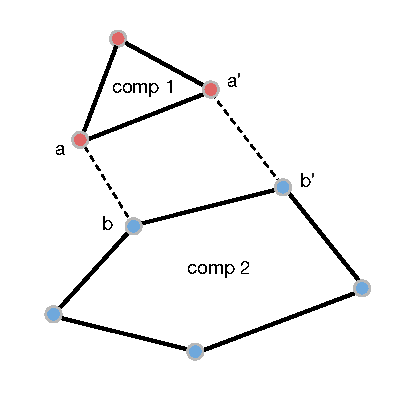
\includegraphics[width=\linewidth]{media/HEU-1__.pdf}
     \caption{First case: before merging}
  \end{subfigure}
  \begin{subfigure}[b]{0.49\linewidth}
    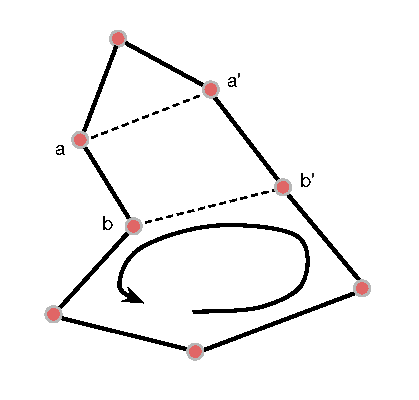
\includegraphics[width=\linewidth]{media/HEU-solved2prova.pdf}
    \caption{First case: after merging}
  \end{subfigure}
  \begin{subfigure}[b]{0.49\linewidth}
    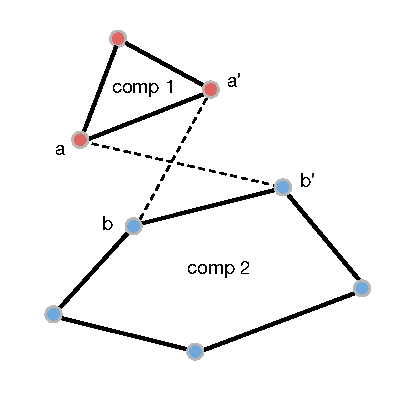
\includegraphics[width=\linewidth]{media/HEU-2_.pdf}
    \caption{Second case: before merging}
  \end{subfigure}
  \begin{subfigure}[b]{0.49\linewidth}
    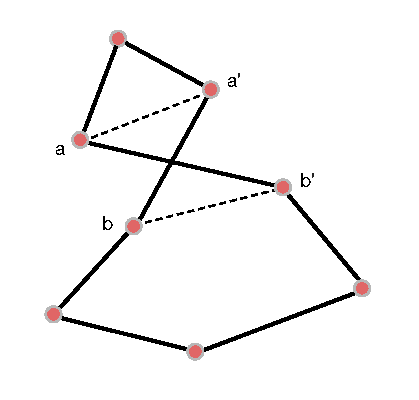
\includegraphics[width=\linewidth]{media/HEU-2solved2prova.pdf}
    \caption{Second case: after merging}
  \end{subfigure}
  \caption{The two ways to merge connected components used by the complete\_tour algorithm.}
  \label{fig:completetour}
\end{figure}
\clearpage
\noindent
Since the overall Algorithm \ref{alg:completetouralg} is $O(n^2)$, the Heuristic Callback is called only when the depth of the decision tree is less than or equal to 10.
\subsection{Generic Callback}
The Generic Callback is a relatively new function that contains essentially two new features with respect to previous callbacks.
The first one is that the callback, during a call to a user-defined function, doesn't stop the execution of the \textit{Dynamic Search} algorithm. The latter is a branch-and-cut based algorithm, kept secret by CPLEX, which guarantees better performance than the traditional but robust branch-and-cut algorithm.
The second feature is that with a single callback we can define each previous callback by using the \textit{context}. The context is a CPLEX structure that defines in which part of the brach-and-cut algorithm the solver calls the callback.
An example of the use of Generic Callback is presented in Algorithm \ref{alg:genlazycall}.  This algorithm includes the three callbacks implemented in Algorithm \ref{alg:heucall}, namely, Lazy Callback, UserCut Callback and Heuristic Callback. 
The solver calls the Generic Callback function with the context ``CANDIDATE" when an integer solution is found (line 8). In this case, we have simply collected all the functions included in the Lazy Callback and in the Heuristic Callback (lines 9 - 15). On the other hand, after each fractional solution found by the solver the context used is ``RELAXATION" (line 16). In this part of the algorithm, we have collected all the function included in the UserCut Callback together with the Concorde algorithms (lines 17 - 21).

\begin{algorithm}
    \caption{Generic Callback}\label{Generic Callback}
    \hspace*{\algorithmicindent} \textbf{Output:} $\textbf{\textit{z}\text{*}} $ optimal solution to TSP on the input graph $G$
    \begin{algorithmic}[1]
   \Function{TSPopt}{$G = (V,E) , \; c : E \rightarrow \mathbb{R}^+$}
  \State model $ \leftarrow $ \textbf{$\ast$ Initialize variables and objective function $\ast$ }
  \State optimizer $ \leftarrow $ \textbf{$\ast$ Initialize the callback function within the solver $\ast$ }
  \State $\textbf{\textit{z}\text{*}} \gets \text{optimizer(model)}$
  \State \Return \textbf{\textit{z}\text{*}}
\EndFunction
\\
  \Function{GenericCallback}{\textbf{\textit{x}}, context, model}
 
  \If{$ (context = CANDIDATE) $} 
   	\State comp $ \leftarrow $ \textbf{$\ast$ number of components in the integer solution \textit{x} $\ast$ }
	 \If{$ (comp > 1) $} 
	\State \textbf{$\ast$ Add SECs for each connected component to the model $\ast$ }
	\State \textbf{\textit{x}$^{\prime}$} $ \leftarrow $ \text{complete\_tour(\textbf{\textit{x}})}
	\State \textbf{$\ast$ Save \textbf{\textit{x}$^{\prime}$} and the thread index $\ast$ }
	\EndIf  
	\State \textbf{if} $\ast$ there is a solution available in the current thread $\ast$ \textbf{then}
	\State \textbf{$\ast$ Add the TSP heuristic solution \textbf{\textit{x}$^{\prime}$} to the solver $\ast$ }
	\EndIf  
	\If{$ (context = RELAXATION) $} 
   	\State comp $ \leftarrow $ \textbf{$\ast$ number of components in the fractional solution \textit{x} $\ast$ }
	 \If{$ (comp > 1) $} 
	\State \textbf{$\ast$ Add SECs for each connected component to the model $\ast$ }
	\EndIf
		    \algstore{myalg2}
    	\end{algorithmic}
	\label{alg:genlazycall}
   	\end{algorithm}
	\vspace{1cm}
	\begin{algorithm}                   
   	 \begin{algorithmic} [1]              
    	\algrestore{myalg2}
	\If{$ (comp = 1) $} 
	\State \textbf{$\ast$ Add SECs on the separated fractionary solution $\ast$ }
	\EndIf 
	\EndIf  
	\State \Return 
	\EndFunction

    \end{algorithmic}
    \end{algorithm}

\subsection{Final comparison between callbacks}
\label{callbackresults}
For the final comparison of the callbacks we used the same dataset described in Section \ref{LMcomparision}, i.e. 30 instances with four random seeds, for a total of 120 problems.
For the comparison we used two metrics: time elapsed and nodes solved. The first metric is used to compare the time spent by the algorithms to compute the optimal solution of each problem. The second metric is used to compare the number of nodes solved by the algorithms when running the branch-and-cut algorithm. The number of nodes solved can make us understand if the cuts applied by the callbacks are sufficient to prevent the expansion of numerous nodes of the branched tree during the branch-and-cut algorithm. \\
On Figure \ref{fig:lazy} it is possible to see the performance profile of the Legacy Callbacks. In CPLEX the legacy callbacks are the previous version of the new Generic Callback and the \textit{Lazy Callback}, \textit{UserCut Callback} and \textit{Heuristic Callback} are part of this category. The first thing we can notice is that the \textit{Lazy Callback} is the one that performs worst. The \textit{Heuristic Callback} seems to be performing slightly better than the \textit{UserCut Callback}. The heuristic solutions provided to the solver using the Heuristic Callback together with the cuts computed in fractional solutions using Concorde, can significantly reduce the amount of time to compute the optimal solution for the TSP problem. The number of nodes solved by the three algorithms is also consistent with the times, as you can see in Figure \ref{fig:lazynodes}. This confirms that cuts and heuristic solutions are capable of cutting many branches of the decision tree. \\
On Figure \ref{fig:gen} it is possible to see the performance profile of the Generic Callbacks. Also in this case the \textit{Heuristic Callback} outperforms all the other both in terms of time and number of nodes solved, as you can see in Figure \ref{fig:gennodes}. \\
In Figure \ref{fig:allcall} we can see the comparison between all the Callbacks. The \textit{Legacy Heuristic Callback} outperforms the others in most of the instances, however it does not do so consistently. In a small percentage of instances it takes a really long time to finish and is outperformed by the \textit{Generic Heuristic Callback}. This means that if we were to look at the percentage of instances solved quickly, the \textit{Legacy Heuristic Callback} is the best method, but the method capable of solving the most of instances within 4 times the time it takes the fastest method to find the optimum is the \textit{Generic Heuristic Callback}. This is followed by the \textit{Generic UserCut Callback} with slightly worse performance and the \textit{Legacy UserCut Callback}.\\ \textit{Lazy Callbacks} are the ones that perform worst. The number of nodes solved by each algorithm is shown in Figure \ref{fig:allcallnodes}. \\
On Figure \ref{fig:exact} it is possible to see the performance profile of the Exact Algorithms. The only new thing to note is that \textit{Loop Methods} perform better than the \textit{Legacy Lazy Callback}.
All performance profiles are shown on the following pages.

\begin{figure}[h!]
  \centering
  \begin{subfigure}[b]{0.97\linewidth}
    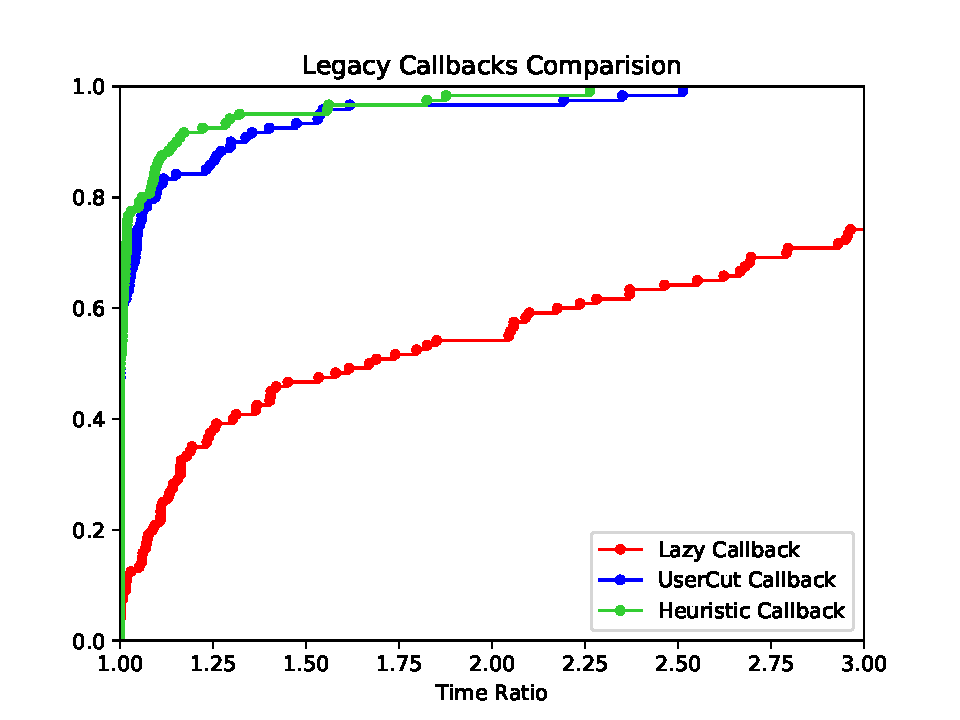
\includegraphics[width=\linewidth]{media/LegacyCallbacks.pdf}
  \end{subfigure}
  \begin{subfigure}[b]{0.97\linewidth}
  \ContinuedFloat
    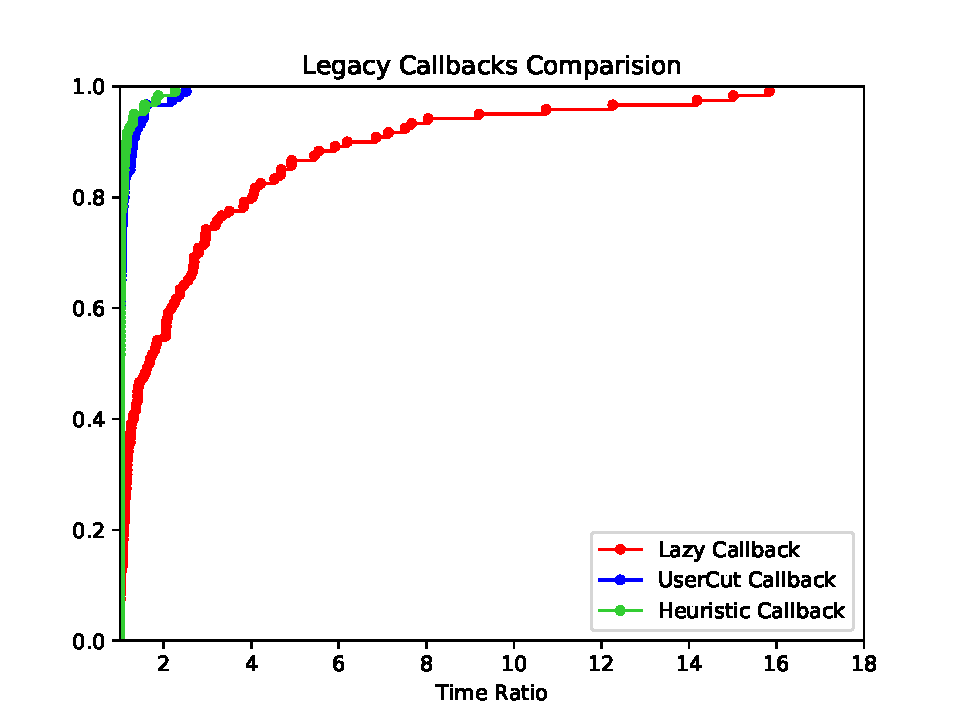
\includegraphics[width=\linewidth]{media/LegacyCallbacks1.pdf}
  \end{subfigure}
  \caption{On top: detailed view of the performance profile of Legacy Callbacks. \\On the bottom: full view of the performance profile of Legacy Callbacks.}
\label{fig:lazy}
\end{figure}

\begin{figure}[h!]
  \centering
  \begin{subfigure}[b]{0.97\linewidth}
    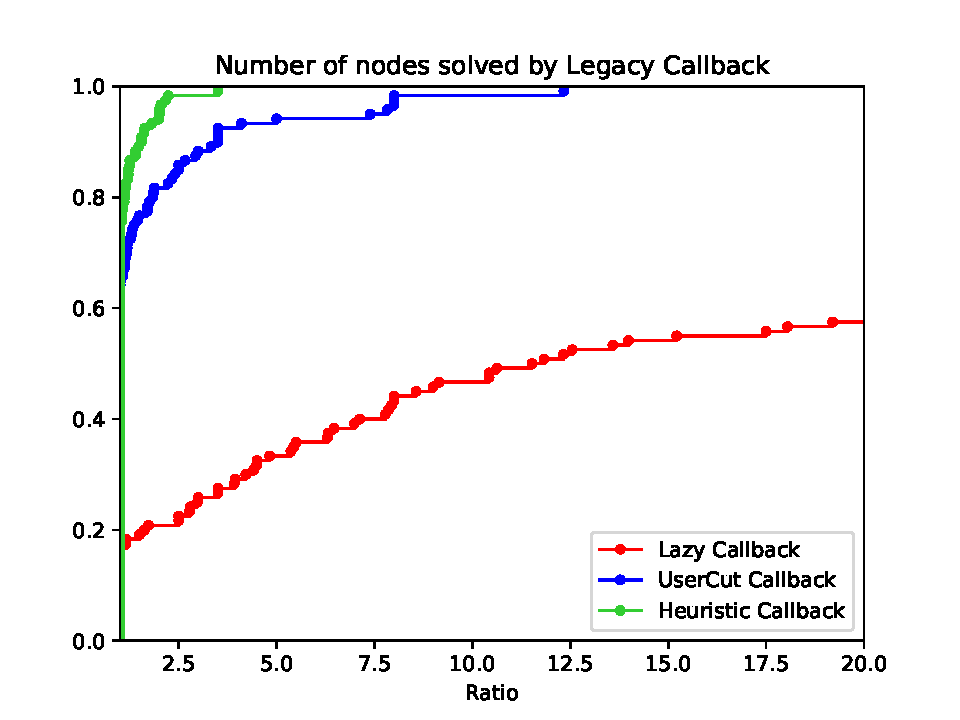
\includegraphics[width=\linewidth]{media/NodesLegacy.pdf}
  \end{subfigure}
  \begin{subfigure}[b]{0.97\linewidth}
  \ContinuedFloat
    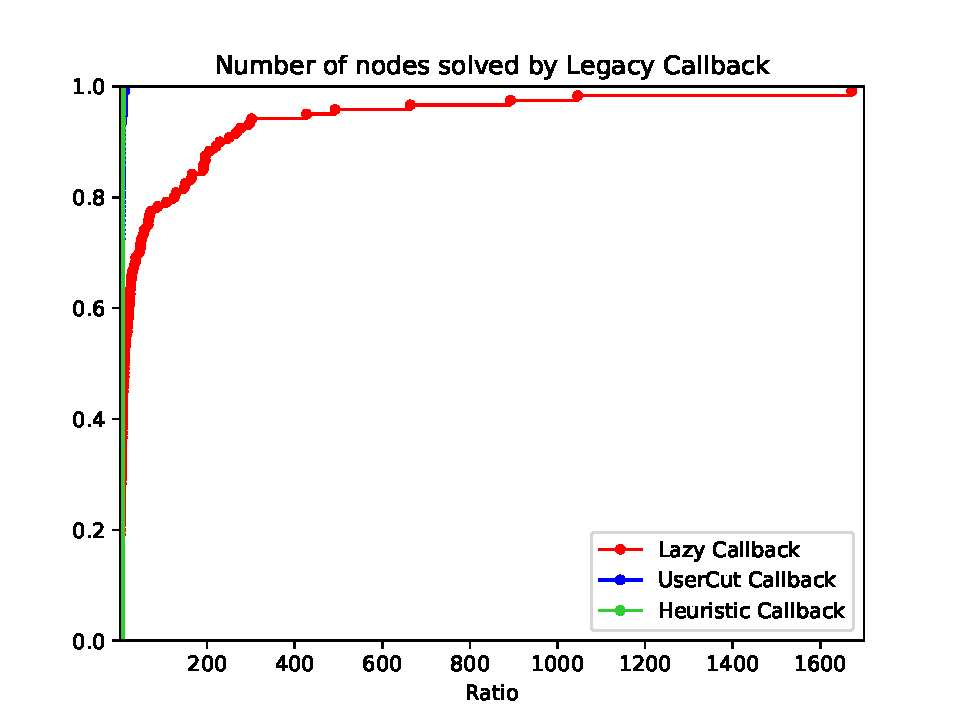
\includegraphics[width=\linewidth]{media/NodesLegacy1.pdf}
  \end{subfigure}
  \caption{On top: detailed view of the performance profile of Legacy Callbacks regarding the number of solved nodes. On the bottom: full view of the performance profile of Legacy Callbacks.}
  \label{fig:lazynodes}
\end{figure}

\begin{figure}[h!]
  \centering
  \begin{subfigure}[b]{0.97\linewidth}
    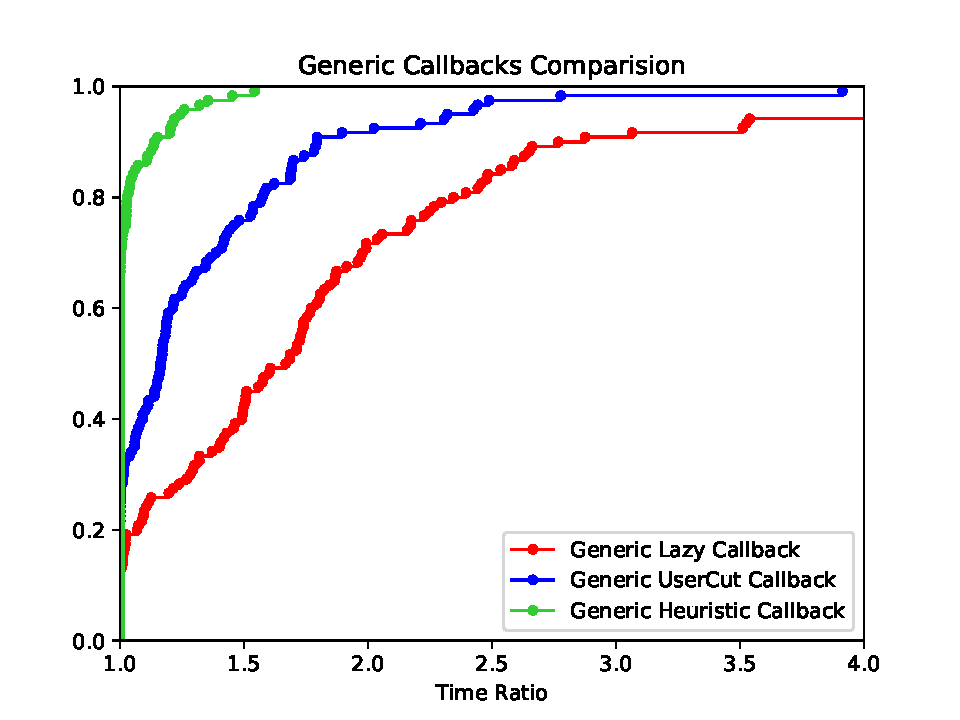
\includegraphics[width=\linewidth]{media/GenericCallbacks.pdf}
  \end{subfigure}
  \begin{subfigure}[b]{0.97\linewidth}
  \ContinuedFloat
    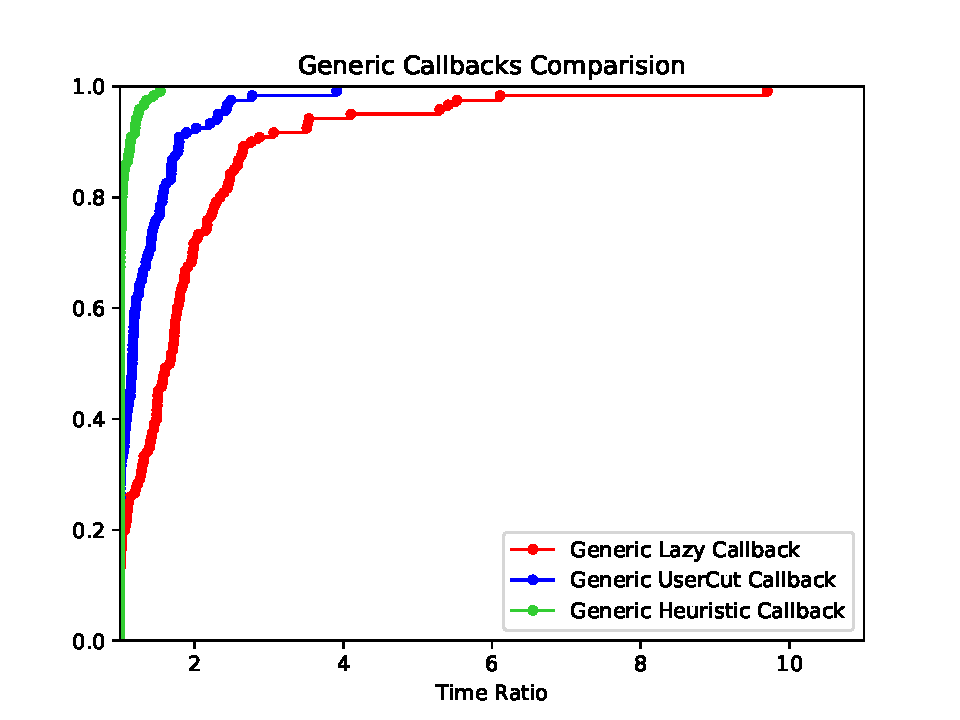
\includegraphics[width=\linewidth]{media/GenericCallbacks1.pdf}
  \end{subfigure}
  \caption{On top: detailed view of the performance profile of Generic Callbacks. \\On the bottom: full view of the performance profile of Generic Callbacks.}
  \label{fig:gen}
\end{figure}

\begin{figure}[h!]
  \centering
  \begin{subfigure}[b]{0.97\linewidth}
    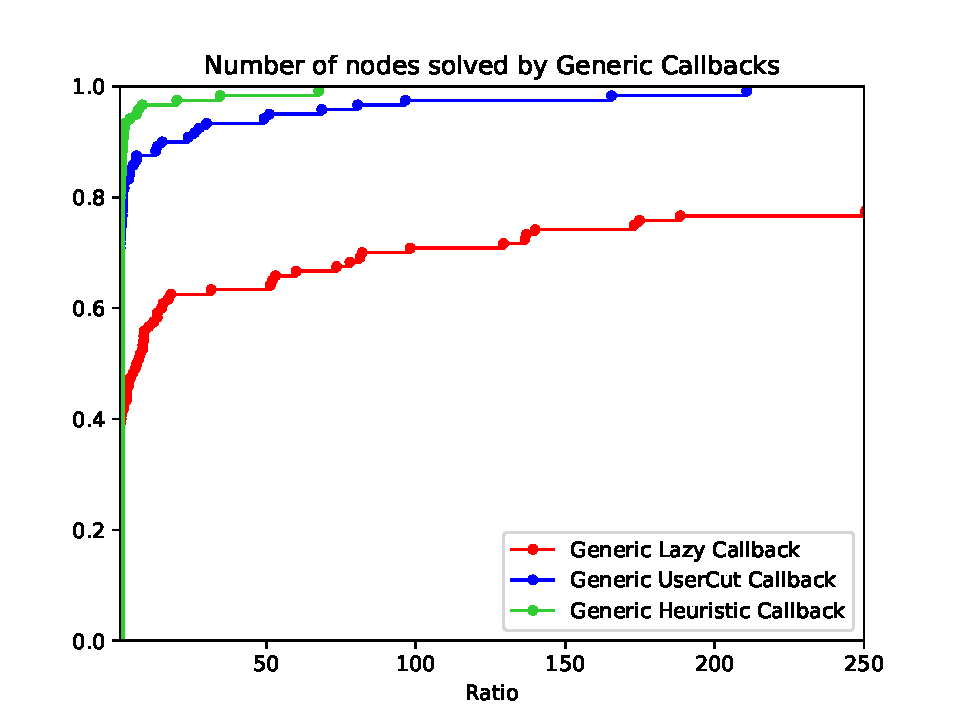
\includegraphics[width=\linewidth]{media/NodesGeneric.pdf}
  \end{subfigure}
  \begin{subfigure}[b]{0.97\linewidth}
  \ContinuedFloat
    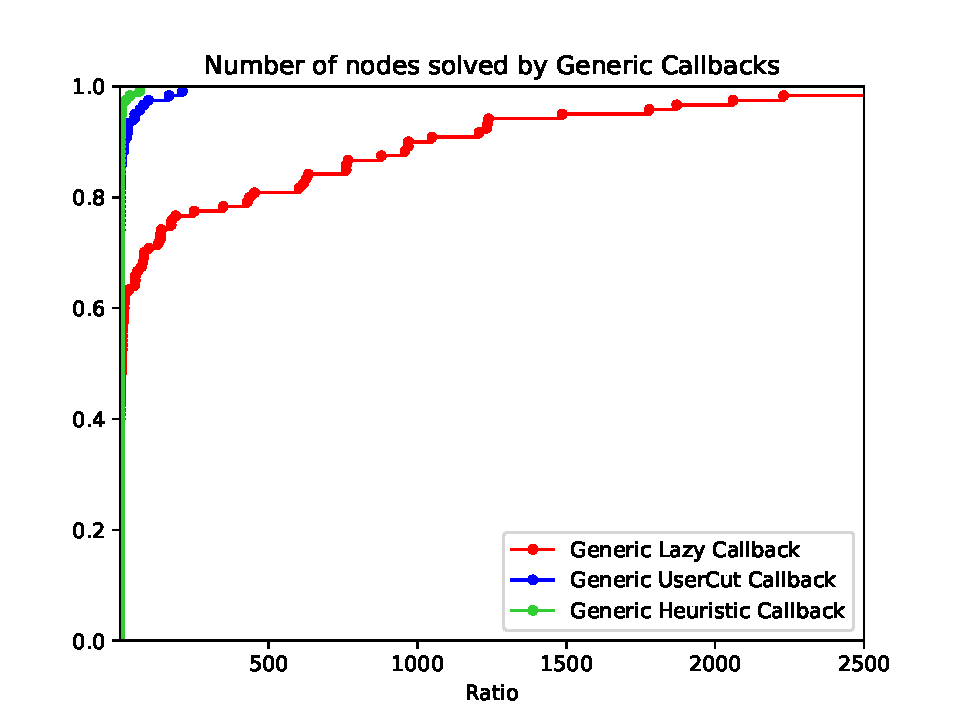
\includegraphics[width=\linewidth]{media/NodesGeneric1.pdf}
  \end{subfigure}
  \caption{On top: detailed view of the performance profile of Generic Callbacks regarding the number of solved nodes. On the bottom: full view of the performance profile of Generic Callbacks.}
    \label{fig:gennodes}
\end{figure}

\begin{figure}[h!]
  \centering
  \begin{subfigure}[b]{0.97\linewidth}
    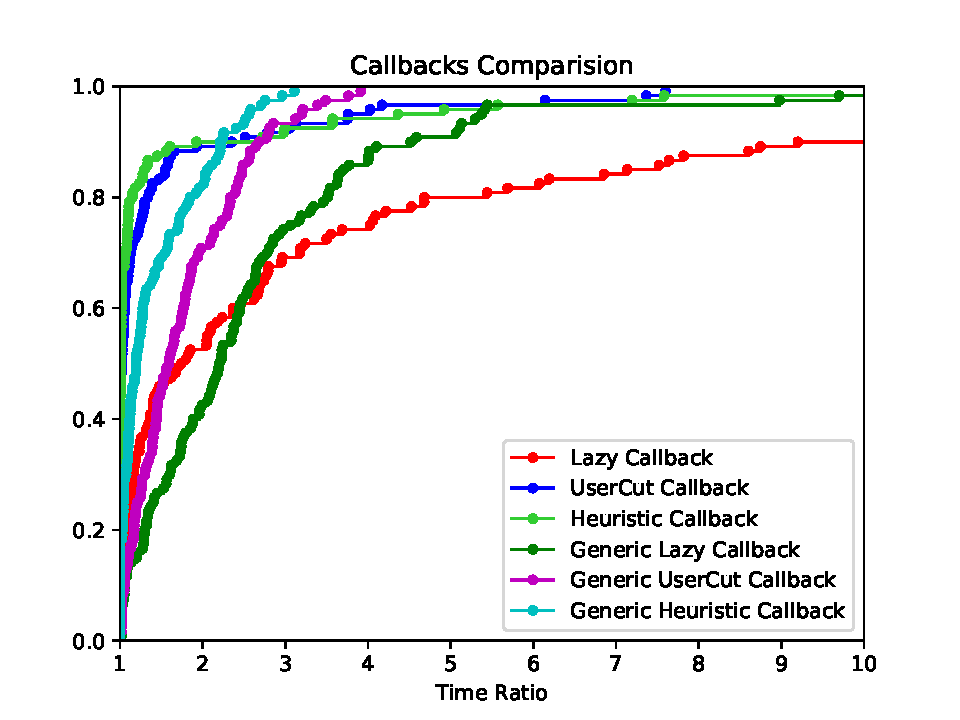
\includegraphics[width=\linewidth]{media/AllCallbacks.pdf}
  \end{subfigure}
  \begin{subfigure}[b]{0.97\linewidth}
  \ContinuedFloat
    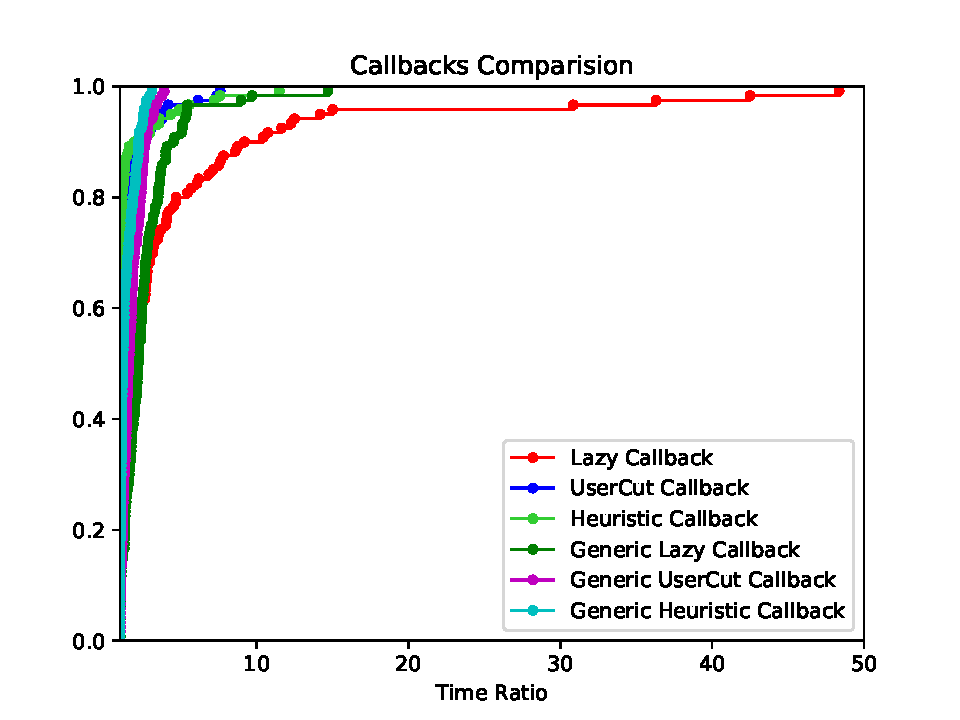
\includegraphics[width=\linewidth]{media/AllCallbacks1.pdf}
  \end{subfigure}
  \caption{On top: detailed view of the performance profile of all Callbacks. \\On the bottom: full view of the performance profile of all Callbacks.}
      \label{fig:allcall}
\end{figure}

\begin{figure}[h!]
  \centering
  \begin{subfigure}[b]{0.97\linewidth}
    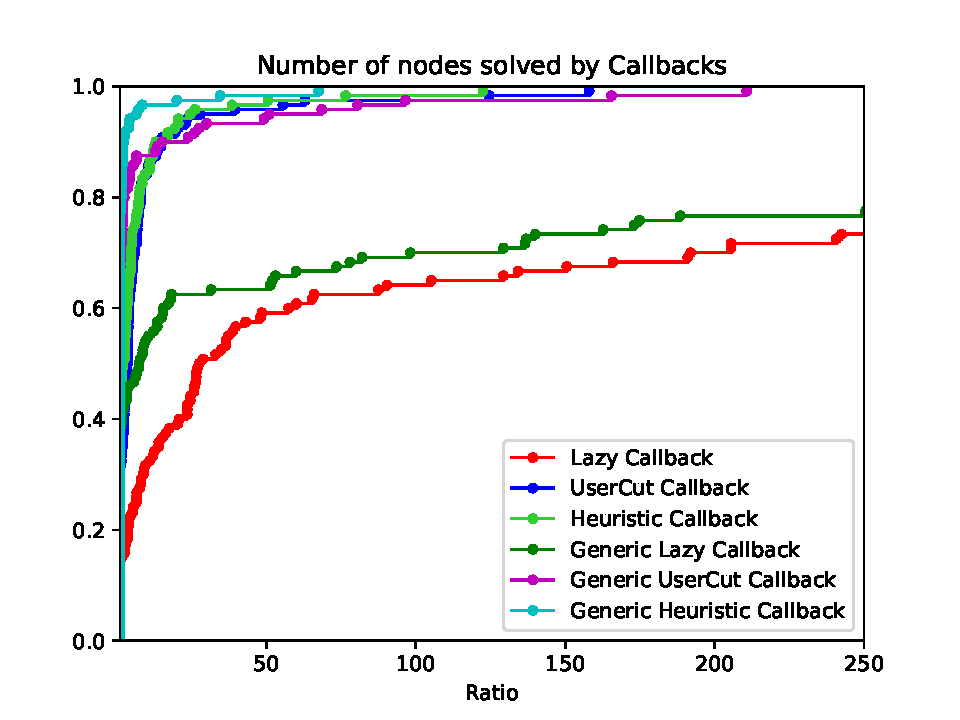
\includegraphics[width=\linewidth]{media/NodesAll.pdf}
  \end{subfigure}
  \begin{subfigure}[b]{0.97\linewidth}
  \ContinuedFloat
    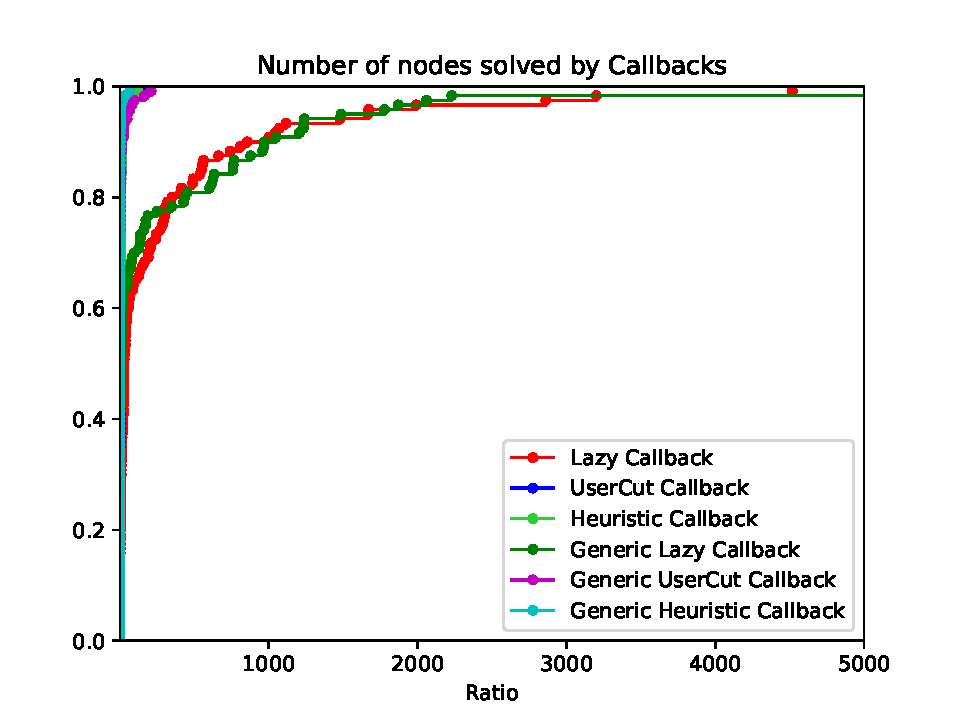
\includegraphics[width=\linewidth]{media/NodesAll1.pdf}
  \end{subfigure}
  \caption{On top: detailed view of the performance profile of all Callbacks regarding the number of solved nodes. On the bottom: full view of the performance profile of all Callbacks.}
       \label{fig:allcallnodes}
\end{figure}

\begin{figure}[h!]
  \centering
  \begin{subfigure}[b]{0.97\linewidth}
    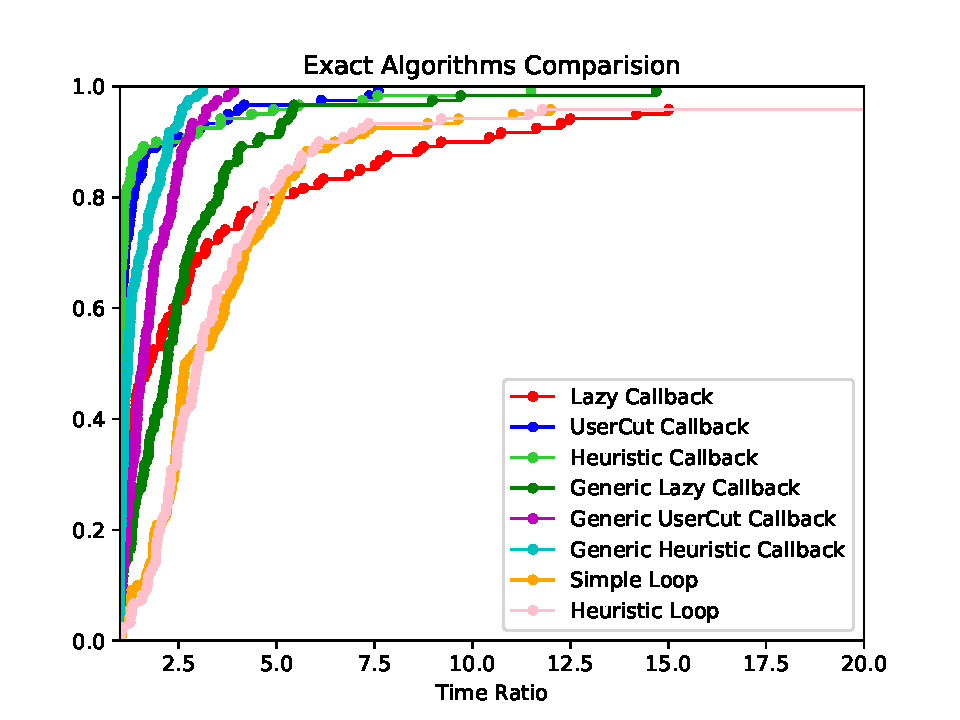
\includegraphics[width=\linewidth]{media/Exact.pdf}
  \end{subfigure}
  \begin{subfigure}[b]{0.97\linewidth}
  \ContinuedFloat
    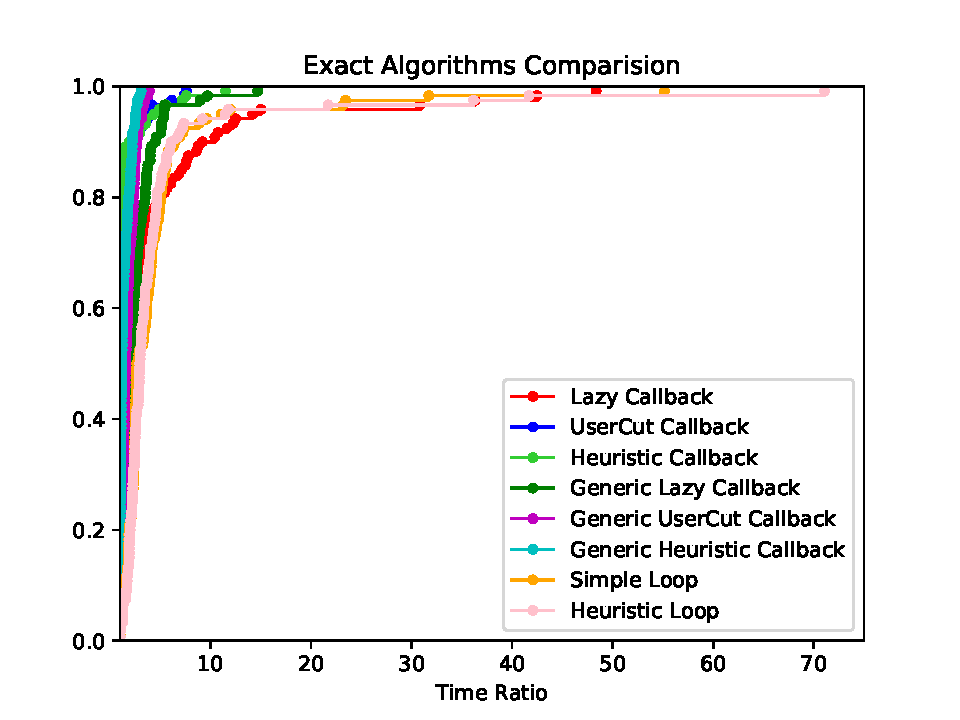
\includegraphics[width=\linewidth]{media/Exact1.pdf}
  \end{subfigure}
  \caption{On top: detailed view of the performance profile of Exact Algorithms. \\On the bottom: full view of the performance profile of Exact Algorithms.}
      \label{fig:exact}
\end{figure}



\chapter{Matheuristics}
On this chapter we will illustrate two heuristic solution for the TSP problem that are based on CPLEX.

\section{Hard fixing}
When we have to resolve a large instance of TSP, CPLEX can require a large amount of time. Moreover in some practical application we may have to resolve the problem in a certain amount of time that we cannot exceed. So for this reason we can set a time limit for CPLEX, that means that the solver will return the best solution found within that limit. The hard fixing algorithm starts from this point. Let's set a time limit (10 minutes for example) and consider the solution obtained. Of course this solution with high probability is not the optimum solution, but it may contains some edges that belong to it. So the idea is to fix some edges, and pass the new model to CPLEX. In order to do this we can simply work on the bounds of the variables: if we set $1 \leq x(i,j) \leq 1$ the corresponding edge is fixed on the solution. The new model of course is simpler, because we have a smaller amount of variables, so when we resolve it with CPLEX (again with a fixed time limit) it may find a better solution. This procedure can also be iterate until a final time limit (like 1 hour) is reached: each time we release the variables that were fixed on the previous iteration (just reset the bounds to $0 \leq x(i,j) \leq 1$) and we choose a new set of edges to fix.
Note that when the variables are fixed, due to the fact that the instance is smaller, CPLEX may resolve that model to its optimum before the time limit exceed.
Of course the choice of which edge to fix and their number is quite relevant. In general a good idea is to set a fixing percentage and randomly choose the variables to fix. We can also decide to variate the percentage over the iterations, for example starting with an high value (like 90\%) and then decrease it until zero. This mean that on the initial iterations the problem to resolve is very small so we may get a significant improve, while on the last iterations we have a big problem but lot of freedom to refine the solution. Of course this is only an example and other strategies can be implemented.  
\\\\ Our implementation of the Hard Fixing is presented in Algorithm \ref{alg:hf}. 
We used two variables to manage the time limit of the algorithm. The variable \textit{remaining\_time} keeps track of the time left to the algorithm to compute the solution. At beginning the variable assumes the value of the original time limit given by the user (line 2). The variable \textit{time\_x\_cycle} is the inner time limit and it is initially fixed to \textit{time\_limit/5} (line 3). Since with the inner time limit is very hard that an initial good solution will be computed, we provide to CPLEX a heuristic solution builded with the algorithm GRASP and refined with the 2-OPT algorithm (lines 4-6).
The algorithm then proceeds solving the problem within a while loop (line 7). At each iteration, we initially set the inner time limit as CPLEX environment parameter (lines 8 - 11). 
Then the solution, within the time limit, is computed (line 13) with the time needed to compute it (lines 12 and 14).
At this point, the variable \textit{remaining\_time} is updated subtracting from it the time taken by the solver (line 15).
\\ The variable \textit{percentage}, initially set to 90\% (line 1), is updated only if after two consecutive iterations the solution found doesn't improve of at least the 10\%. The update consists in subtracting 15\% from the previous percentage of fixed variables (line 18). Then the algorithm proceeds by resetting the lower bound of all variables to 0.0 (line 19), randomly selecting the indices of variables to be fixed and setting the lower bound of them to 1.0 (line 20). This sequence is repeated as long as the user-set time limit is reached.

\begin{algorithm}
    \caption{Hard Fixing}\label{Hard Fixing}
    
    \hspace*{\algorithmicindent} \textbf{Input:} $G = (V,E) , c : E \rightarrow \mathbb{R}$\\
    \hspace*{\algorithmicindent} \textbf{Output:} A solution for the TSP problem
    \begin{algorithmic}[1]
    \State $\textit{percentage} \gets \textit{0.9}$
    \State $\textit{remaining\_time} \gets \textit{timelimit}$
    \State $\textit{time\_x\_cycle} \gets \textit{timelimit / 5}$
    \State model $ \leftarrow $ \textbf{$\ast$ Initialize variables and objective function $\ast$ }
    \State first\_solution $ \leftarrow $ \textbf{$\ast$ Heuristic solution with GRASP + 2-OPT $\ast$ }
    \State model $ \leftarrow $  CPXaddmipstarts(first\_solution)
    \While {(\textit{remaining\_time} $>$ 0)} 
    	\If{$ (\textit{remaining\_time} > \textit{time\_x\_cycle})$} 
	\State $ model \gets $ CPX\_PARAM\_TILIM$(\textit{time\_x\_cycle}) $
	
	\Else \State $ model \gets $ CPX\_PARAM\_TILIM$(\textit{remaining\_time}) $
	\EndIf
	
	\State $\textit{t1} \gets \textit{second()}$
    	\State $\textbf{\textit{x}} \gets \text{solution}(\text{model}) $\;
	\State $\textit{t2} \gets \textit{second()}$
	\State $\textit{remaining\_time} \gets \textit{remaining\_time $-$ (t2 $-$ t1)}$
	\If{$ (\textit{remaining\_time} <= 0)$} 
	\State \textbf{break}
	\EndIf
	\State \textbf{$\ast$ If the solution doesn't improve (+10\%) twice in succession then $ percentage $ $ -$= $ 0.15. $ $\ast$}
	\State \textbf{$\ast$ Restore the default bounds for each variable $\ast$}
	\algstore{myalg}
    	\end{algorithmic}
	\label{alg:hf}
   	\end{algorithm}
	
	\begin{algorithm}                     
   	 \begin{algorithmic} [1]              
    	\algrestore{myalg}
	\State \textbf{$\ast$ Hard fixing of each variable according to \textit{percentage} $\ast$}
    \EndWhile
    \State \textbf{return} \textbf{\textit{x}} 
    \end{algorithmic}
    \end{algorithm}

\section{Local branching}
The strategy of this algorithm \cite{LB} is similar to the one of hard fixing: each iteration fix some edges in order to give to CPLEX a simpler version of the problem. However, rather then randomly choose the variable to fix, we let CPLEX decide which edges to maintain. We can achieve this with the introduction of a new constraint: let's consider an initial solution H provided by CPLEX within a time limit, let $x_e^H$ be the variables equals to one on this solution, we want the sum of these variables to be greater or equals than a percentage of the total number of edges. More formally:
\begin{equation*}
	\sum_{e \in E, \; x_e^H = 1} x_e \geq \alpha n
\end{equation*}
where $\alpha$ is the selected percentage and n is the size of the instance. In other word with this constraint we are telling CPLEX that we want a percentage of variables that are in the initial solution to be also in the final solution. At this point we can give the new model to CPLEX that will resolve it within the time limit, automatically deciding which variables to maintain.
Of course this is not a valid constraint for the problem, cause we are not sure that the variables equals to one on a solution belong to the optimum.\\
Again we can iterate the procedure, each time removing the old constrain and generating a new one, based on the new solution, until a final time limit is reached. The fact that the selection of the variables to fix is not random, means that the CPLEX solution is deterministic, so it is not wise to execute two iterations with the same fixing percentage, cause we may resolve two times the same problem obtaining the same solution within the time limit.
Finally, another shrewdness that is required, is that this algorithm works only if the fixing percentage is very high, so iteration with percentage of 50-60 or less should be avoided. 
\\\\ Our implementation of the Local branching is presented in Algorithm \ref{alg:lb}. The implementation is pretty similar to Algorithm \ref{alg:hf}, for this reason we only emphasise the differences between the two algorithms. 
At each iteration of the while loop (line 7), the variables of the solution are saved and a new local branching constraint is added to the model, removing the previous one. The known term of the constraint, that is the variable \textit{percentage} in the algorithm, is initially set to: number of nodes $\ast$ 0.95 (line 1) and is updated with the same conditions as Algorithm \ref{alg:hf}, but in this case subtracting from the variable \textit{percentage} the value: number of nodes $\ast$ 0.05 (lines 18 - 21). As in algorithm \ref{alg:hf}, the sequence is repeated as long as the user-set time limit is reached.

\begin{algorithm} [H]
    \caption{Local branching}\label{Local branching}
    \hspace*{\algorithmicindent} \textbf{Input:} $G = (V,E) , c : E \rightarrow \mathbb{R}$\\
    \hspace*{\algorithmicindent} \textbf{Output:}  A solution for the TSP problem
    \begin{algorithmic}[1]
    \State $\textit{percentage} \gets \textit{$|$V $|$ $\ast$ $0.95$}$
    \State $\textit{remaining\_time} \gets \textit{timelimit}$
    \State $\textit{time\_x\_cycle} \gets \textit{timelimit / 5}$
    \State model $ \leftarrow $ \textbf{$\ast$ Initialize variables and objective function $\ast$ }
    \State first\_solution $ \leftarrow $ \textbf{$\ast$ Heuristic solution with GRASP + 2-OPT $\ast$ }
    \State model $ \leftarrow $  CPXaddmipstarts(first\_solution)
    \While {(\textit{remaining\_time} $>$ 0)} 
    	\If{$ (\textit{remaining\_time} > \textit{time\_x\_cycle})$} 
	\State $ model \gets $ CPX\_PARAM\_TILIM$(\textit{time\_x\_cycle}) $
	
	\Else \State $ model \gets $ CPX\_PARAM\_TILIM$(\textit{remaining\_time}) $
	\EndIf
	\State $\textit{t1} \gets \textit{second()}$
    	\State $\textbf{\textit{x}} \gets \text{optimal\_solution}(\text{model}) $\;
	\State $\textit{t2} \gets \textit{second()}$
	\State $\textit{remaining\_time} \gets \textit{remaining\_time $-$ (t2 $-$ t1)}$
	\If{$ (\textit{remaining\_time} <= 0)$} 
	\State \textbf{break}
	\EndIf
	\State \textbf{$\ast$ If the solution doesn't improve (+10\%) twice in succession then $ percentage $ $ -$= $ (0.05 \ast percentage).$ $\ast$}
	\State \textbf{$\ast$ Save the indices of the solution variables. $\ast$}
	\State \textbf{$\ast$ If is not the first cycle remove the last row of the model. $\ast$}
	\State \textbf{$\ast$ Add the new local branching constraint with $\alpha n = percentage. $ $\ast$}
    \EndWhile
    \State \textbf{return} \textbf{\textit{x}}
    \end{algorithmic}
    \label{alg:lb}
    \end{algorithm}

\section{Final comparison between Matheuristics}
The instances used to compare heuristic algorithms are the following: 

\begin{multicols}{3}
    \begin{itemize}
        \item d657.tsp
        \item d1291.tsp
        \item fl417.tsp
        \item fl1400.tsp
        \item fl1577.tsp
        \item nrw1379.tsp
        \item p654.tsp
        \item pcb1173.tsp
        \item pcb3038.tsp
        \item pr1002.tsp
        \item pr2392.tsp
        \item rl1304.tsp
        \item rl1323.tsp 
        \item rl1889.tsp
        \item u724.tsp
        \item u1060.tsp
        \item u2152.tsp
        \item u2319.tsp
        \item vm1084.tsp
        \item vm1748.tsp
    \end{itemize}
    \end{multicols}
    
\noindent
For each problem $i$ and algorithm $j$, we compare the Gap computed as
\begin{equation}
	gap_{ij} \; (\%) = { objFunc_j(i) - objFunc_{opt}(i) \over objFunc_j(i) } * 100,
\end{equation}
\noindent
where $objFunc_j(i)$ is the objective function value computed by the algorithm $j$ for the problem $i$.
The method used to compute a solution within the time limits is the \textit{Generic Heuristic Callback}, which is the best exact algorithm we implemented (see Section \ref{callbackresults}).
In figure \ref{fig:Math} you can see the performance profile of the Matheuristic algorithms. The Hard Fixing outperforms the Local Branching in most of instances. Even if worse, the Local Branching algorithm achieves a gap within twice the best, so it is considered by us a valid competitor. 
From our experiments we observed that Matheuristics achieve the optimum in several instances, even in a problem with 2319 nodes. We also noticed that Matheuristic algorithms work very well even with big instances, achieving an objective function value within 5\% from optimum. All the numerical results are reported in Section \ref{resultMath}.  \\
The reason for their good performance may be due to the powerful \textit{Generic Heuristic Callback} algorithm which, thanks to Concorde, generates numerous cuts on fractional solutions, and also provides heuristic solutions to the solver thanks to a quick and effective algorithm (see Section \ref{callHeu}). Another reason is that our Matheuristic algorithms exploit all time available by fixing a decreasing number of variables.

\begin{figure}[H]
\centering
	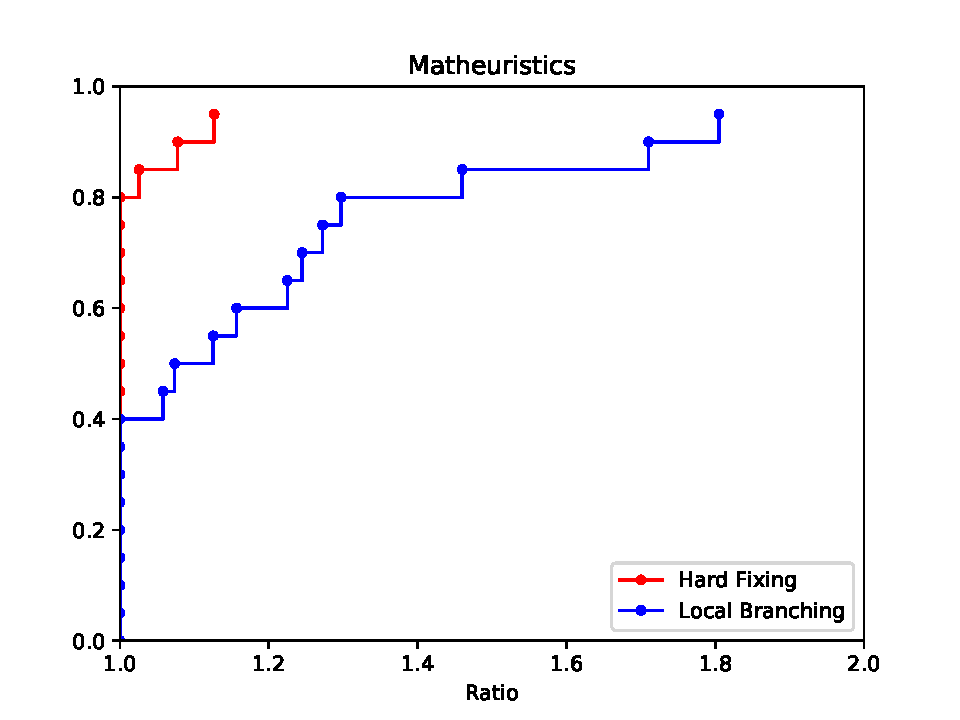
\includegraphics[scale=0.9]{media/Math.pdf} \\
	\caption{Performance profile of Matheuristics}
	\label{fig:Math}
\end{figure}


\chapter{Stand-alone heuristics}
On this chapter we will illustrate some stand-alone heuristics. These algorithms are so called because they provide an heuristic solution without relying on CPLEX or any other solver. The literature in this case is huge: there are plenty of different approaches and each of them can have multiple variations. On this report we will cover some of the major ideas. \\
For all the experiments to collect data for the performance profiles and the comparison between different algorithms we used a dataset of 20 instances, with a size between 400 and 3000 points. A detailed list of all the instances used and their dimension can be found on the tables of the section 5.4.

\section{Heuristic solution builder}
On this section we will illustrate some heuristics algorithm to generate in a rapid way a solution for the TSP problem. Of course the results provided by these algorithms are admissible solutions but not the optimum solution.

\subsection{Nearest neighborhood}
Nearest neighborhood is a greedy algorithm \footnote{algorithm that always makes the choice that looks best at the moment. That is, it makes a locally optimal choice in the hope that this choice
will lead to a globally optimal solution.  %TODO AGGIUNGERE LA FONTE DELLA CITAZIONE	 
} that works in the following way: start from a random point that is considered the first visited node. Then pick as next node the nearest to the last visited (greedy choice) and iterate until all the nodes are visited. This procedure can be repeated until a time limit is reached, each time starting from a different random point, keeping in memory the best solution and eventually update it if a new one is found. The algorithm is pretty simple but provide an admissible solution (that of course is not the best one and in the very most of the cases is quite far from the optimum) in a short time. \\

\begin{figure}[h!]
  \centering
  \begin{subfigure}[b]{0.49\linewidth}
    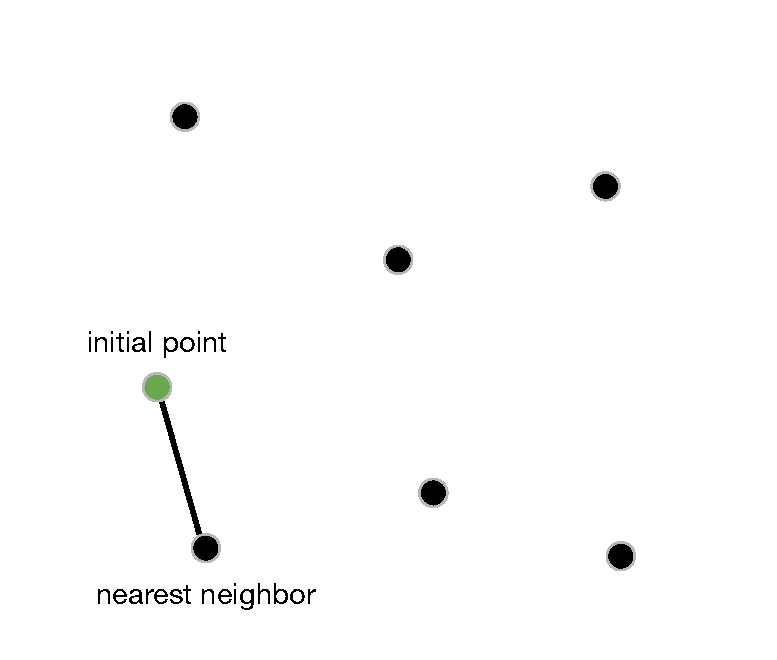
\includegraphics[width=\linewidth]{media/fase1.pdf}
     \caption{Initial step}
  \end{subfigure}
  \begin{subfigure}[b]{0.49\linewidth}
    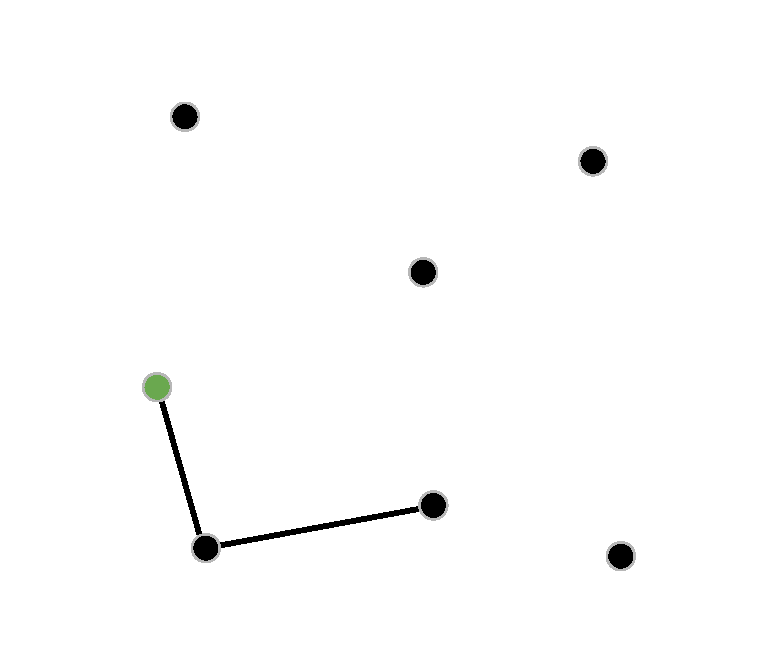
\includegraphics[width=\linewidth]{media/fase2.pdf}
    \caption{Second step}
  \end{subfigure}
  \begin{subfigure}[b]{0.49\linewidth}
    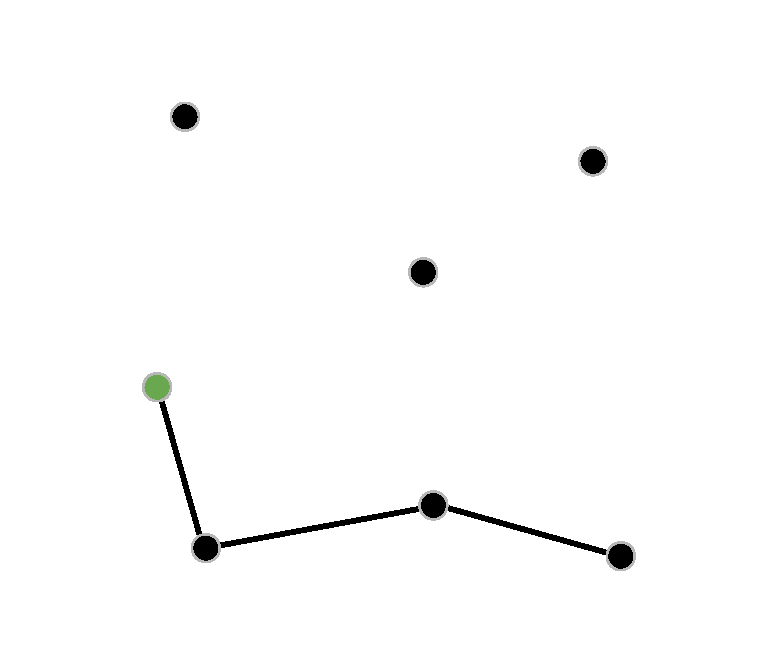
\includegraphics[width=\linewidth]{media/fase3.pdf}
    \caption{Third step}
  \end{subfigure}
  \begin{subfigure}[b]{0.49\linewidth}
    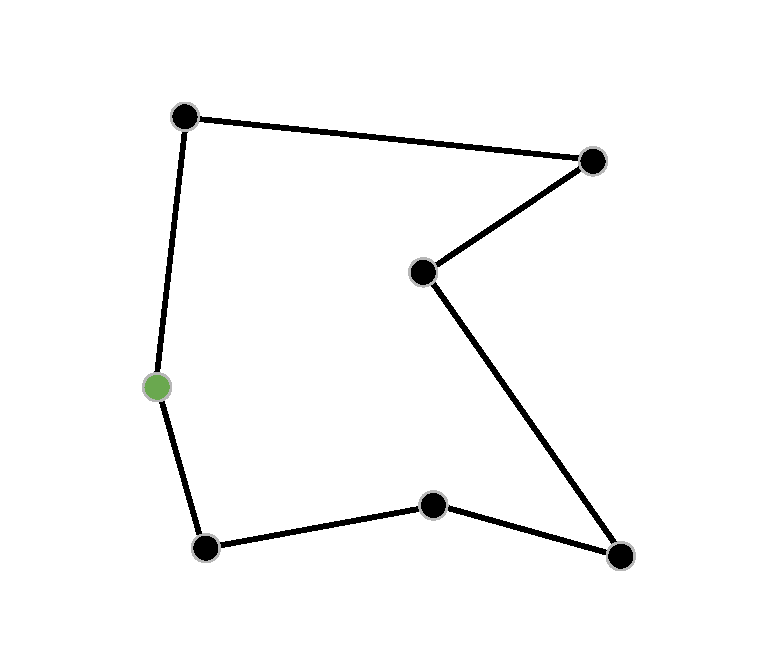
\includegraphics[width=\linewidth]{media/fase4.pdf}
    \caption{Final result}
  \end{subfigure}
  \caption{Execution of nearest neighbor algorithm}
\end{figure}

\noindent On our implementation we decided to trade space for time. Since the operation to compute the nearest point is repeated several time, we decide to store for each point the list of all others points sorted by their distances from that one. This require $O(n^2)$ additional space. Considering the time, instead, to sort the points we implemented a simple \textit{insertion sort}, that is $O(n^2)$, so in total we need an initial $O(n^3)$ (This part could be further improved with a better sort algorithm like \textit{merge sort} that is $O(n \cdot log(n))$, but since the initial time to order the nodes on our experiments was negligible, we decided to use insertion sort that was easier to implement). So, by paying this initial cost we were able to speed up each iteration of nearest neighborhood, in fact each time we needed to find the nearest point we just had to pick the first available one from the ordered list. Of course in the worst case this is $O(n)$, because it can happen that the firsts elements of the ordered list have already been visited, so I have to run across most of the list until I find an available point. However, what we saw in practice is that, except when there are left few nodes to visit, the first available element is always on the firsts position of the ordered list so the operation to find the nearest neighbor became $\Theta(1)$ in most of the cases (for example, we tried on multiple instances between 100 and 500 points and the average number of access to the ordered list to find the nearest point was between 3 and 6). \\

\noindent The major problem of this technique is that visiting always the next closest point leads to the creation of lots of intersection between edges, that of course are inefficient. A possible solution to improve this initial result will be shown on the next section dedicated to the refining algorithms. \\
Another problem is that this algorithm is deterministic, so this mean that if it is run twice starting from the same initial point, it produce the same solution. The consequence of this is that the number of different circuit that it can explore is limited to the total number of nodes.

\subsection{GRASP}
GRASP is a variation of nearest neighborhood that introduce a random component. On each iteration, rather than picking the nearest point to the last visited, select the three closest points and choose one of them at random as next visited vertex. 
(Or alternatively assign a different probability to each of the three points, for example 0.6 to the closest point and 0.3 and 0.1 respectively to the second and the third).

\begin{algorithm}
	\caption{GRASP}\label{GRASP method}
	\hspace*{\algorithmicindent} \textbf{Input:} Instance I of the TSP \\
	\hspace*{\algorithmicindent} \textbf{Output:} Admissible solution for the instance
    \begin{algorithmic}[1]
    		\State \textit{cost(bestSolution) $\leftarrow \infty$}
		\While{! termination condition}
			\State S $\leftarrow$ empty list
			\State notVisitedList $\leftarrow$ all vertices
			\State currentVertex $\leftarrow$ pick 1 random vertex from I
			\State notVisitedList $\leftarrow$ remove(currentVertex) 
			\State S $\leftarrow$ add(currentVertex)
			\For{$i = 1$, $i < N$, i++}
				\State v1, v2, v3 $\leftarrow$ pick 3 closest and not visited vertex from currentVertex
				\State nextVertex $\leftarrow$ choose at random one between v1, v2, v3
				\State notVisitedList $\leftarrow$ remove(nextVertex) 
				\State S $\leftarrow$ add(nextVertex)
				\State currentVertex $\leftarrow$ nextVertex
			\EndFor
			\If{cost(S) $<$ cost$($bestSolution$)$}
				\State bestSolution $\leftarrow$ S
			\EndIf
		\EndWhile 
		\State \textbf{return} S
    \end{algorithmic}
\end{algorithm}

\noindent Our implementation was almost the same of nearest neighborhood, with the construction for each point of the initial list of all other points sorted by their distance from that point, with the only difference that first three available points are picked from the list, rather than only one, and the next visited point is chosen at random from them. 
The introduction of the random component means that the probability to repeat the same sequence starting from the same point is very minimal, so GRASP can explore lots of different circuit resolving the problem of determinism of nearest neighborhood. 

\begin{figure}[h!]
  \centering
  \begin{subfigure}[b]{0.49\linewidth}
    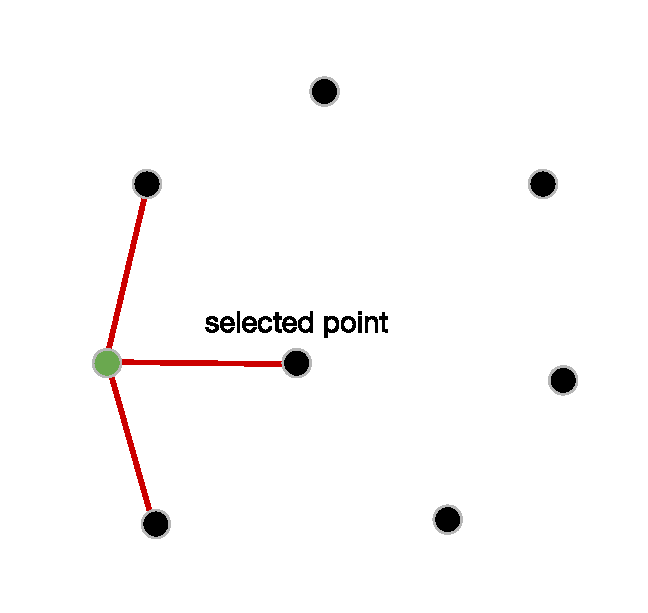
\includegraphics[width=\linewidth]{media/grasp_fase1.pdf}
     \caption{Initial step}
  \end{subfigure}
  \begin{subfigure}[b]{0.49\linewidth}
    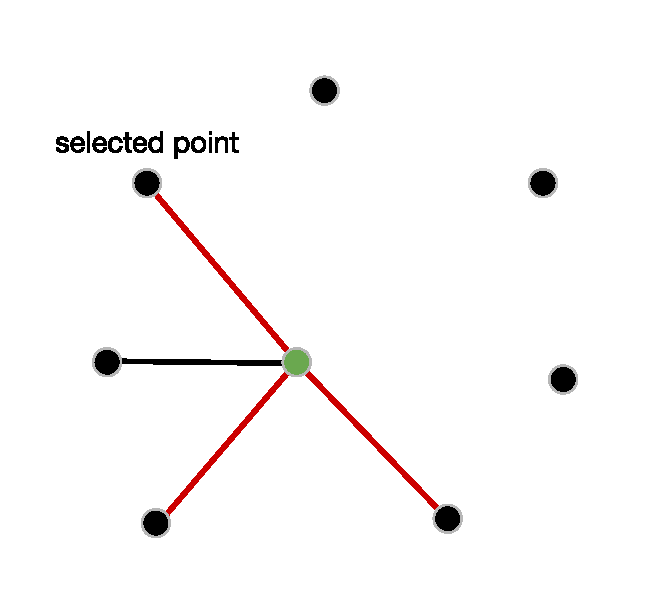
\includegraphics[width=\linewidth]{media/grasp_fase2.pdf}
    \caption{Second step}
  \end{subfigure}
  \begin{subfigure}[b]{0.49\linewidth}
    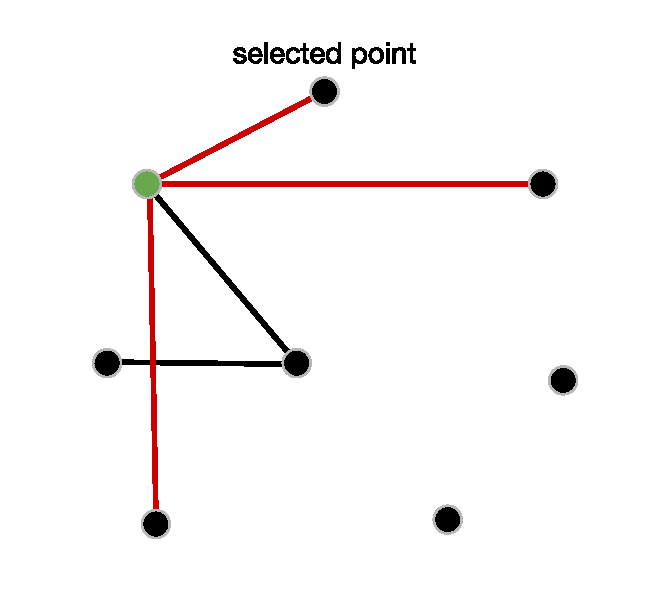
\includegraphics[width=\linewidth]{media/grasp_fase3.pdf}
    \caption{Third step}
  \end{subfigure}
  \caption{Execution of 3 steps of GRASP. Each time the 3 closest points are considered and one is picked at random.}
\end{figure}

\subsection{Insertion heuristic}
This algorithm starts from a simple circuit made with only two points. At each iteration, for each of the remaining vertices to insert, compute the minimal extra mileage. The extra mileage is the cost to insert a point on the circuit. So, for example, if we want to insert the vertex z between vertex x and vertex y, the extra mileage is: $c_{xz} + c_{zy} - c_{xy}$, where $c_{ij}$ is the cost of the edge (i, j). The fact that for each point we search the minimal extra mileage means that we are looking to the best position where insert that point. Insert vertex that has the best extra mileage into the partial circuit and repeat the procedure until all the points are inserted (Figure \ref{fig:insertion}). The algorithm than can be executed several time to explore new solutions, starting every time from different initial points and updating the incumbent if necessary. \\
The cost to compute the best extra mileage is $O(n^2)$, so this mean that the entire algorithm is $O(n^3)$.\\
It is also possible to add the GRASP rule, so rather then selecting the point with the best extra mileage, find the three smallest extra mileages and choose at random between them, in this way the algorithm doesn't converge to the same solution starting from the same initial circuit. \\

\begin{algorithm}
	\caption{Insertion heuristic}\label{Insertion method}
	\hspace*{\algorithmicindent} \textbf{Input:} Instance I of the TSP \\
	\hspace*{\algorithmicindent} \textbf{Output:} Admissible solution for the instance
    \begin{algorithmic}[1]
    		\State \textit{cost(bestSolution) $\leftarrow \infty$}
		\While{! termination condition}
			\State S $\leftarrow$ empty list
			\State S $\leftarrow$ add 2 initial vertices
			\While{! all point are inserted}
				\State bestExtraMileage $\leftarrow \infty$
				\For{\textbf{each} point p to insert}
					\State minExtraMileage $\leftarrow \infty$
					\For{\textbf{each} edge e $\in$ S}
						\State extraMileage $\leftarrow$ computeExtraMileage(p, e)
						\If{extraMileage $<$ minExtraMileage}
							\State minExtraMileage $\leftarrow$ extraMileage
						\EndIf
					\EndFor
					\If{minExtraMileage $<$ bestExtraMileage}
						\State bestExtraMileage $\leftarrow$ minExtraMileage
					\EndIf
				\EndFor
				\State S $\leftarrow$ insert point with bestExtraMileage in the best poisiton
			\EndWhile
			\If{cost(S) $<$ cost(bestSolution)}
				\State bestSolution $\leftarrow$ S
			\EndIf
		\EndWhile 
		\State \textbf{return} bestSolution
    \end{algorithmic}
\end{algorithm}

\begin{figure}[h!]
  \centering
  \begin{subfigure}[b]{0.49\linewidth}
    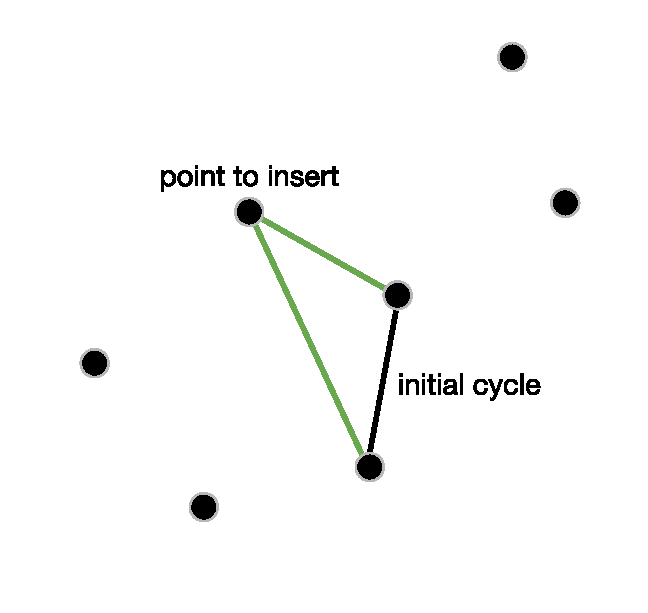
\includegraphics[width=\linewidth]{media/insertion1.pdf}
     \caption{Initial step}
  \end{subfigure}
  \begin{subfigure}[b]{0.49\linewidth}
    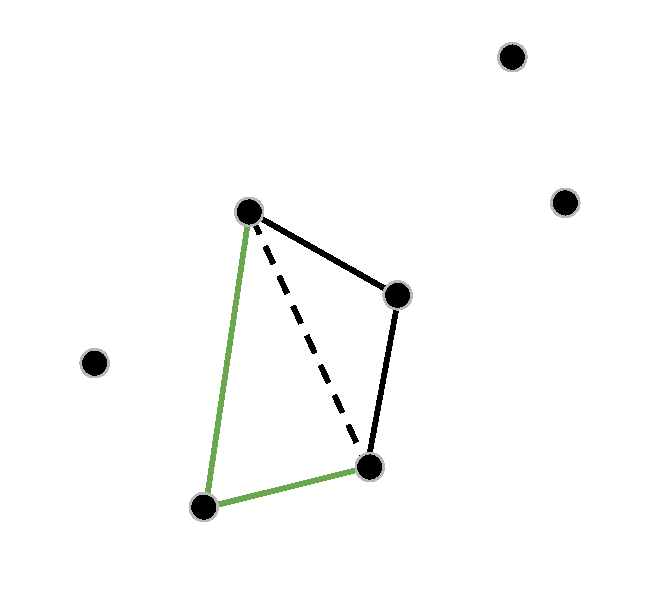
\includegraphics[width=\linewidth]{media/insertion2.pdf}
    \caption{Second step}
  \end{subfigure}
  \begin{subfigure}[b]{0.49\linewidth}
    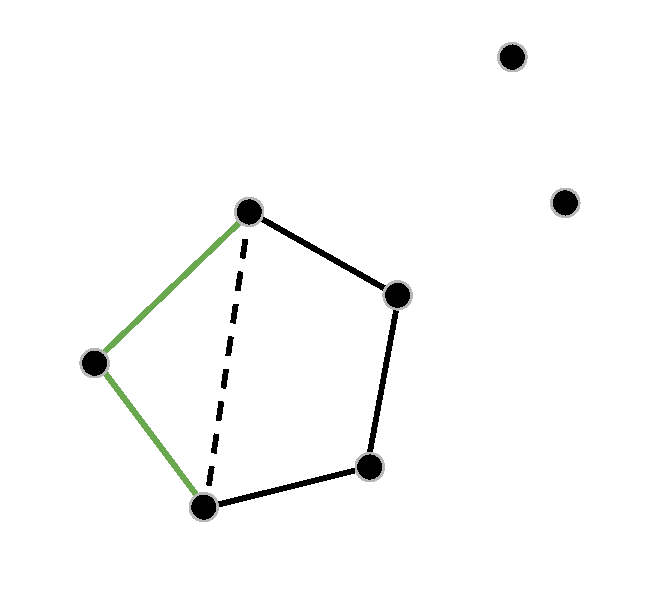
\includegraphics[width=\linewidth]{media/insertion3.pdf}
    \caption{Third step}
  \end{subfigure}
  \begin{subfigure}[b]{0.49\linewidth}
    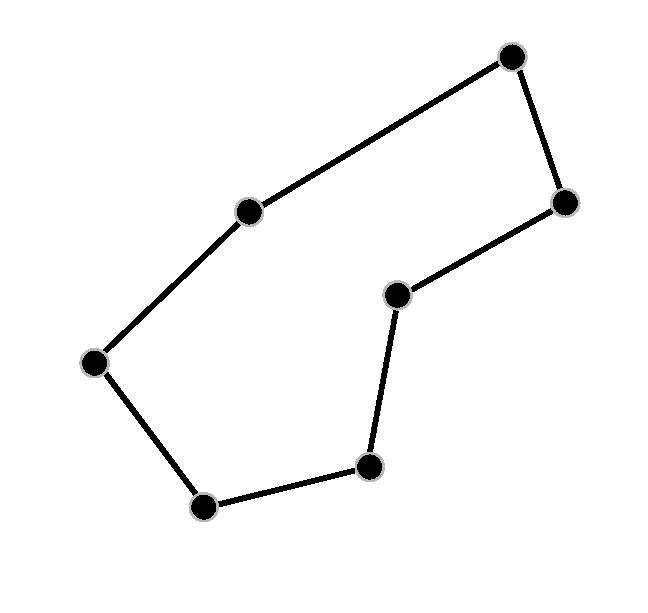
\includegraphics[width=\linewidth]{media/insertion4.pdf}
    \caption{Final result}
  \end{subfigure}
  \caption{Execution of insertion heuristic algorithm}
  \label{fig:insertion}
\end{figure}

\noindent On our implementation to select the initial circuit we decided to pick at random one point and then to select the furthest point from that one. (Of course this is not the only solution: other possibility are, for example, to pick a vertex and its closest one, or to choose two points completely at random.) I addition, at the beginning of the algorithm, we built a matrix where the element i j contains the distance between vertices i and j (So in total we payed an additional $O(n^2)$ in space). We made this choice because on this algorithm distances between points are computed several times and in addition the same distance can be calculated more than once.\\


\subsection{Insertion with convex hull}
This is a variation of the insertion algorithm. It works in the same way but the initialization is different: rather than starting from an initial cycle made of two random points, compute the convex hull \footnote{In geometry, the convex hull or convex envelope or convex closure of a shape is the smallest convex set that contains it. %TODO AGGIUNGERE CITAZIONE WIKIPEDIA 
} of the instance. Then iterate and insert all the remaining points, that are all inside the convex hull, in the same way of Insertion heuristic (Figure \ref{fig:insertionHull}).\\
On our implementation, to find the initial convex hull, we used the Graham Scan algorithm, freely provided by the website www.geeksforgeeks.org. This algorithm is $O(n \cdot log(n))$ and it is performed only once at the beginning so it doesn't impact the overall execution time for the insertion that is $O(n^3)$ as explained on the previous subsection. For more information about the Graham Scan consult \url{https://www.geeksforgeeks.org/convex-hull-set-2-graham-scan/}

\begin{figure}[h!]
  \centering
  \begin{subfigure}[b]{0.8\linewidth}
    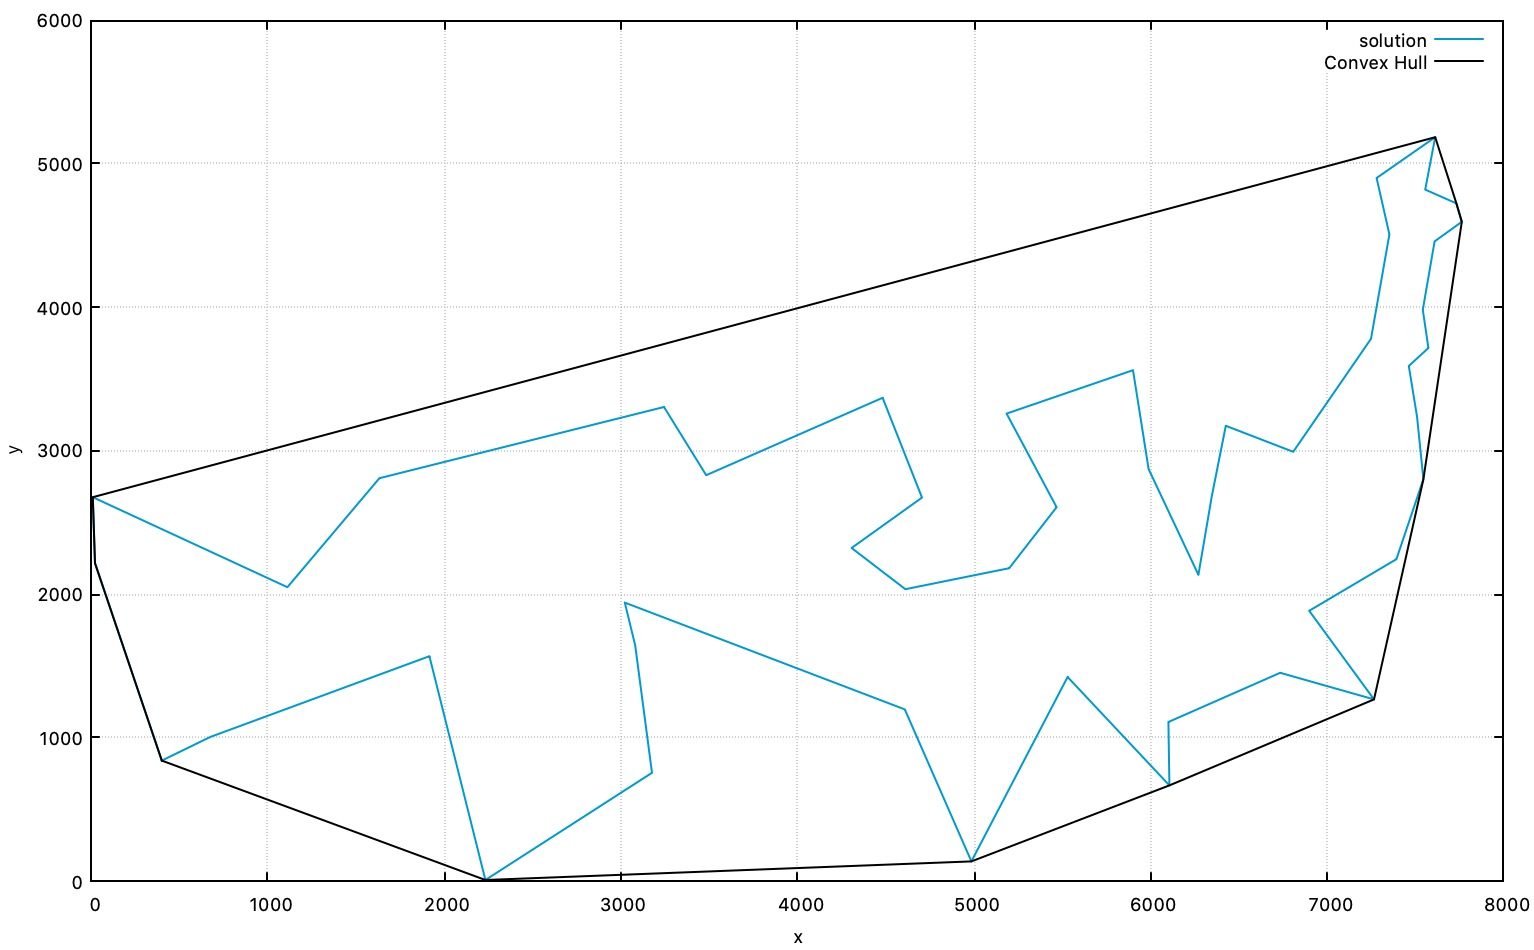
\includegraphics[width=\linewidth]{media/convex1.jpg}
     \caption{problem att48}
  \end{subfigure}
  \begin{subfigure}[b]{0.8\linewidth}
    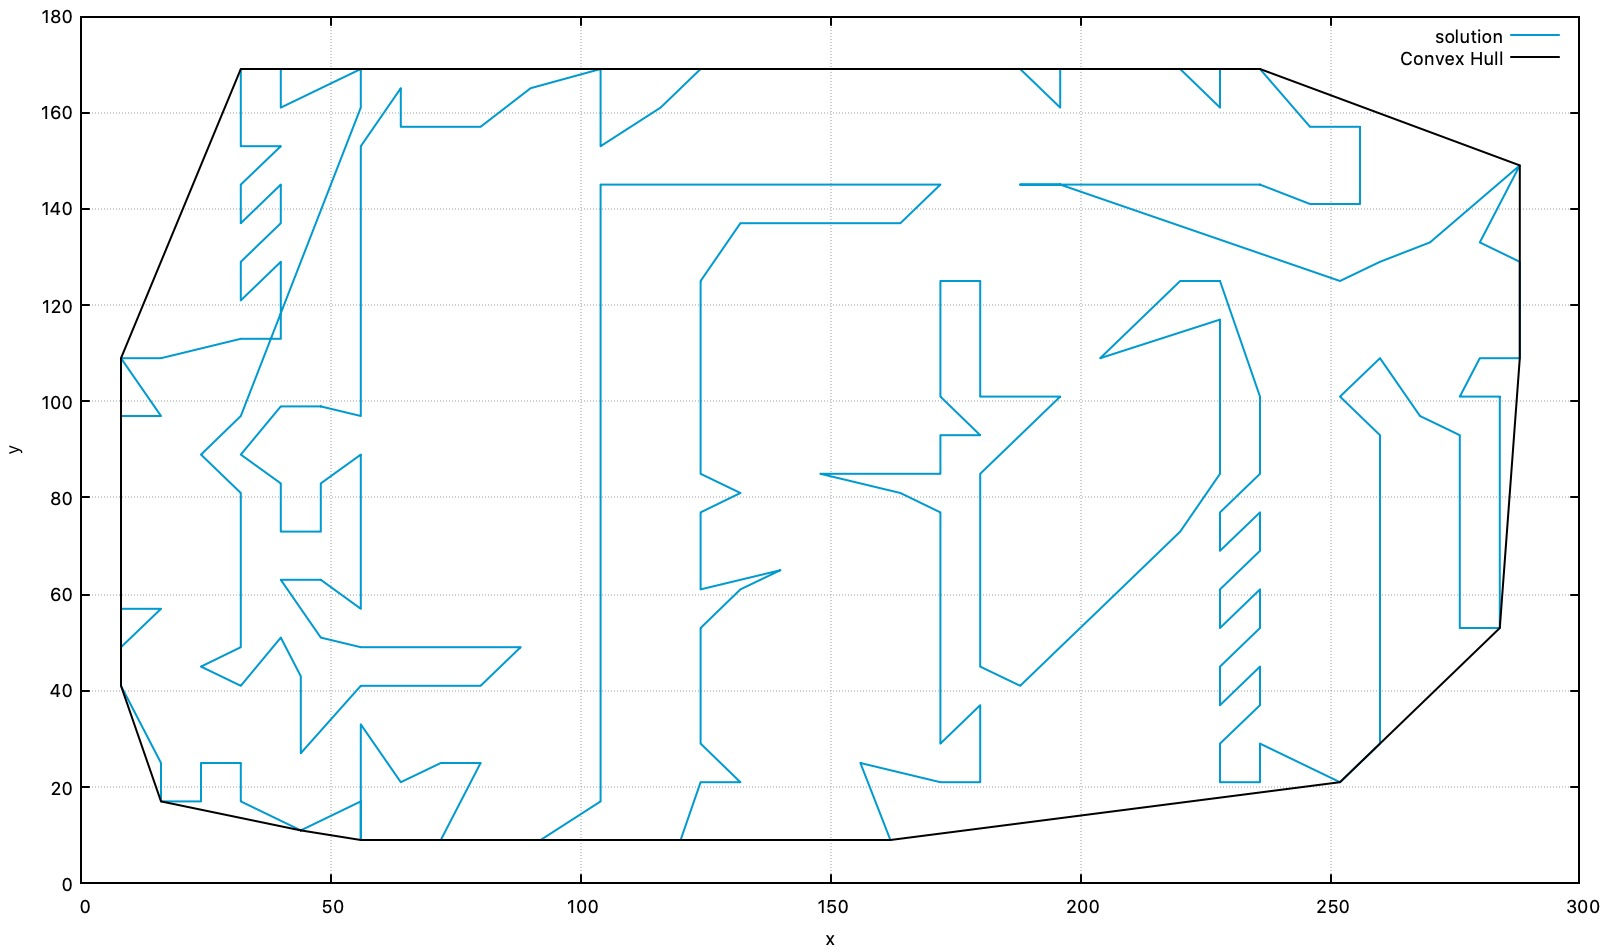
\includegraphics[width=\linewidth]{media/convex2.jpg}
    \caption{problem a280}
  \end{subfigure}
  \caption{Execution of the insertion with convex hull on 2 different problems. It is possible to see the initial convex hull and the final result when all the points inside it are inserted}
  \label{fig:insertionHull}
\end{figure}

\subsection{Final comparison between solution builder}

\begin{figure}[h!]
	\centering
	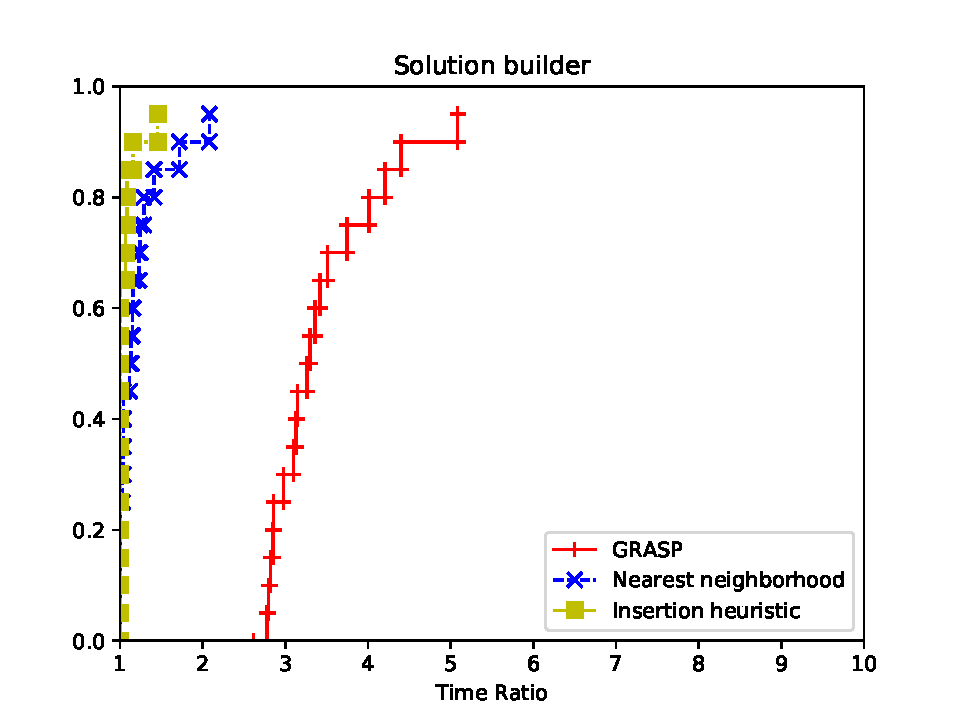
\includegraphics[scale=0.8]{media/builder.pdf}
	\caption{Performance profile of the solution builders}
	\label{fig:solbuilder}
\end{figure}
\noindent
On Figure \ref{fig:solbuilder} the final confrontation between the heuristic solution builders. To obtain these result we test the algorithms on the dataset of 20 instances with a time limit of 5 minutes. 

\clearpage
%\newpage

\section{Refining algorithms}
Refining algorithm are so called because they start from an admissible solution that could by provided by any other algorithm and they try to improve it with a series of iteration.

\subsection{TWO-OPT}
The first algorithm we present is TWO-OPT (or 2-OPT). To explain this technique, let's consider two edges, the first delimited by vertices a and b and with cost $c_{ab}$, the second delimited by c and d and with cost $c_{cd}$ (Both edges belong to an admissible solution provided by any algorithm). Now let's remove these edges and reconnect the vertices in a different way: as result we obtain the edges a, c and b, d with cost respectively $c_{ac}$ and $c_{bd}$. Now lets compute: 
\begin{equation*}
\Delta = c_{ab} + c_{cd} - (c_{ac} + c_{bd})
\end{equation*}
that is the cost of the initial removed edges minus the cost of the new edges. If $\Delta > 0$, it means that the new edges are better than the older and the swap is worth because it reduce (improve) the objective function. Of course the new solution produced is still admissible (Figure \ref{fig:twoopt}).\\

\begin{figure}[h!]
\centering
	\begin{tabular}{@{}cccc@{}}
		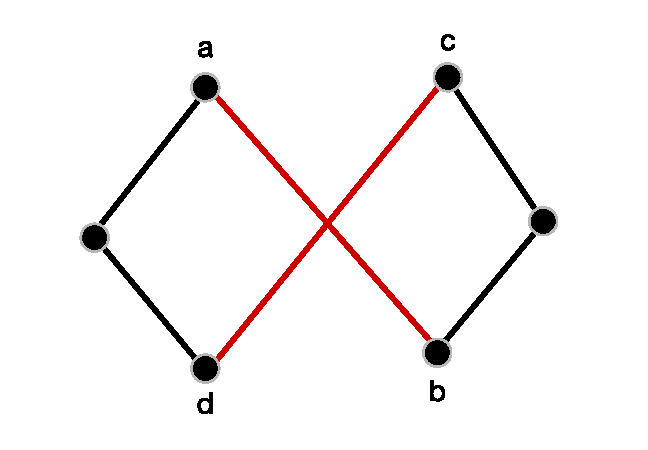
\includegraphics[scale=0.6]{media/twopt1.pdf} &
		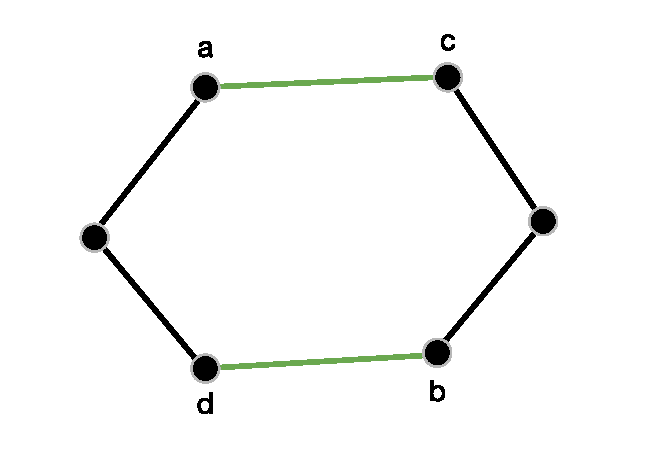
\includegraphics[scale=0.6]{media/twopt2.pdf} \\
	\end{tabular}
	\caption{The 2-OPT move, edges in red are removed and replaced by green edges.}
	\label{fig:twoopt}
\end{figure}

\noindent 2-OPT works in this way: start from an admissible solution, consider all the possible couple of edges (that are in total $O(n^2)$) and for each of them compute the $\Delta$ (That can be calculated in $\Theta(1)$). Then pick the largest $\Delta$, remove the relative edges and reconnect the vertices as previously explained. After this operation, one of the two parts of the cycle that has been divided by the swap, need to be retraced in order to invert the visit sequence of the vertices and reconnect it to the new edge (This is $O(n)$, but since it is done after a $O(n^2)$ doesn't change the overall cost of the swap). Repeat the procedure until all the $\Delta$ are negative, or a fixed time limit is reached.\\

\begin{algorithm}
	\caption{2-OPT}\label{2-OPT method}
	\hspace*{\algorithmicindent} \textbf{Input:} Admissible solution S \\
	\hspace*{\algorithmicindent} \textbf{Output:} Best solution found
    \begin{algorithmic}[1]
		\While{! termination condition}
			\State best$\Delta \leftarrow \infty$
			\For {\textbf{each} couples of edge $v_{ab}$, $v_{cd} \in S$}
				\State $\Delta \leftarrow c_{ab} + c_{cd} - (c_{ac} + c_{bd})$ 
				\If{$\Delta < Best\Delta$}
					\State best$\Delta \leftarrow \Delta$
				\EndIf
			\EndFor
			\If{best$\Delta > 0$}
				\State $S \leftarrow$ perform move with best$\Delta$
			\Else
				\State \textbf{return} S
			\EndIf
		\EndWhile
		\State \textbf{return} S
    \end{algorithmic}
\end{algorithm}

\noindent On our implementation we followed the procedure described above, with the addition of a matrix to store all the distances between points, to avoid to recompute them more than once.\\
This algorithm is very good to remove edge intersections, like the ones produced  by nearest neighborhood (or GRASP). Here in Table \ref{tab:twoopt} some examples.\\ 

\begin{table}[h!]
	\begin{center}
		\begin{tabular}{l|c|c|c}
			\textbf{Instance} & \textbf{GRASP} & \textbf{2-OPT} & \textbf{Improve}	\\
			& (5 sec) & (5 sec) & \\
			\hline
			att48 & 41806 & 35522 & 15\% \\
			eil101 & 879 & 691 & 21\% \\
			ch130 & 9801 & 6347 & 35\% \\
			ch150 & 10477 & 7278 & 30\% \\
			a280 & 4546 & 2886 & 36\% \\
			lin318 & 76940 & 46235 & 39\% \\ 
			att532 & 155010 & 97487 & 37\% \\	
			pr1002 & 492311 & 285078 & 42\% \\
		\end{tabular}
		\caption{Values of the objective functions after running on each instance GRASP algorithm for 5 seconds and then 2-OPT for other 5 seconds.}
		\label{tab:twoopt}
	\end{center}
\end{table}

\noindent These results were obtained after running GRASP for five seconds and then refining the solution with 2-OPT for other five seconds. Of course this dataset is very small but it gives the idea of the power of this technique, we have, in fact, a significant improve of the objective function in all the cases. To notice that the improve increase with large problem. \\
It is possible to visualize the action of 2-OPT by plotting the solution before and after the refining like in Figure \ref{fig:grasp}.

\begin{figure}[h!]
\centering
	\begin{tabular}{@{}cccc@{}}
		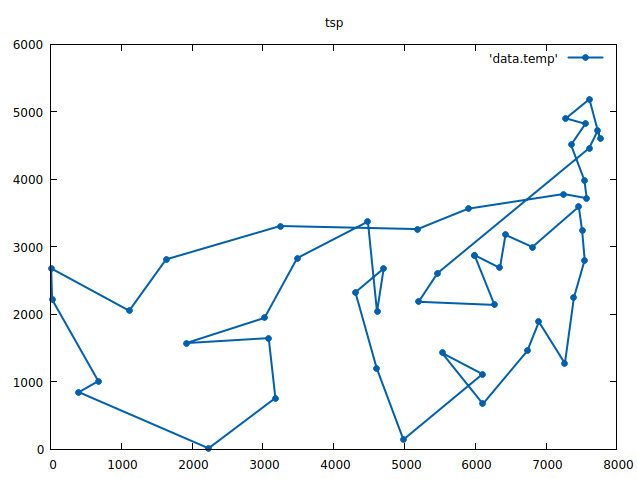
\includegraphics[scale=0.5]{media/before2opt.png} \\
		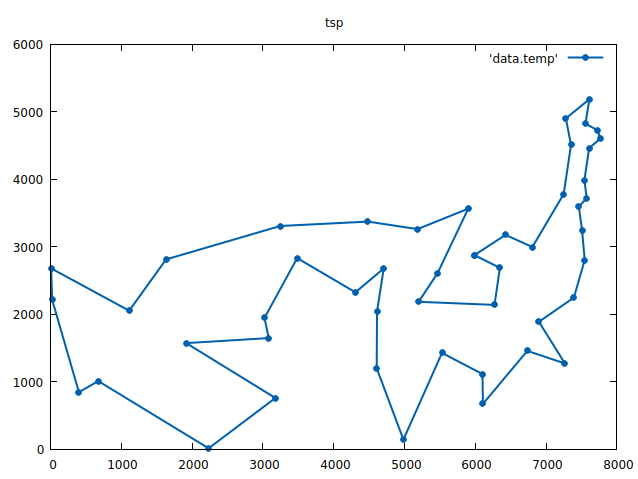
\includegraphics[scale=0.5]{media/after2opt.png} \\
	\end{tabular}
	\caption{Solution of 5 sec of GRASP before (top image) and after (bottom image) a refining of 5 sec}
	\label{fig:grasp}
\end{figure}


\subsection{THREE-OPT}
3-OPT is a variation of 2-OPT that consider 3 edges for the swap rather than only two. This time there are multiple way to reconnect the vertices of the 3 removed edges, in particular for a triad there are 7 possible moves (Figure  \ref{fig:threeopt}). Moreover, we have to consider all the possible triad to find the best one and this is $O(n^3)$. So in general 3-OPT is more complicated to implement and due to the fact that is cubic doesn't work well with big problems, for example with instances with more than 10000 points.

\begin{figure}[h!]
  \centering
  \begin{subfigure}[b]{0.24\linewidth}
    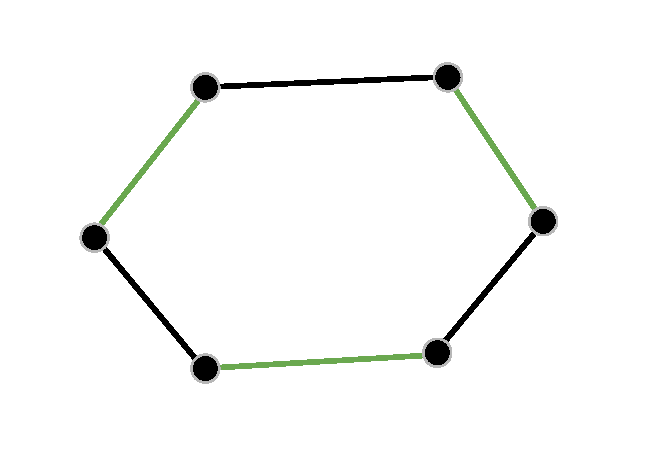
\includegraphics[width=\linewidth]{media/threeopt1.pdf}
     \caption{}
  \end{subfigure}
  \begin{subfigure}[b]{0.24\linewidth}
    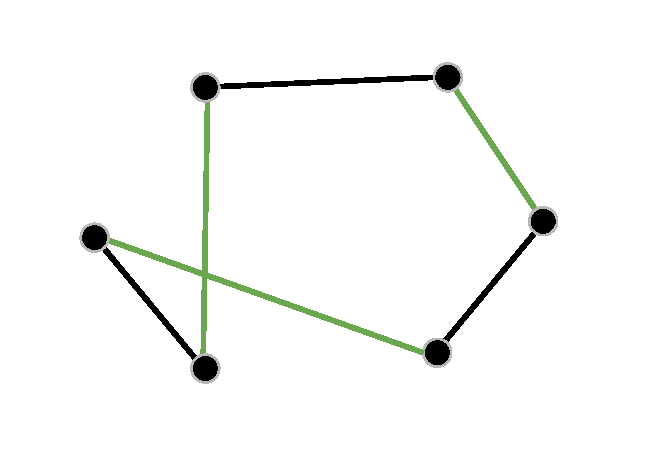
\includegraphics[width=\linewidth]{media/threeopt2.pdf}
    \caption{}
  \end{subfigure}
  \begin{subfigure}[b]{0.24\linewidth}
    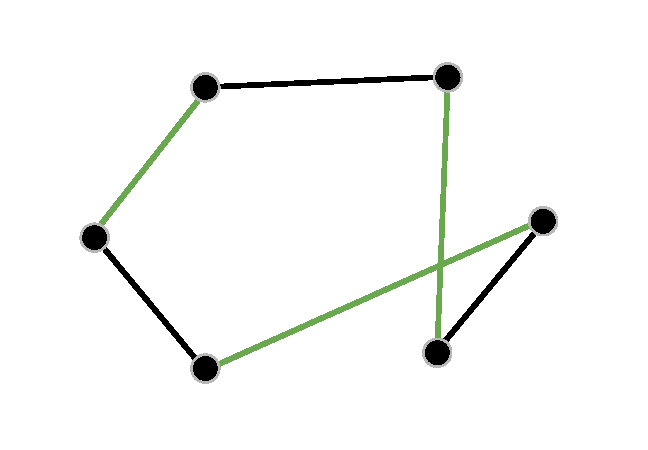
\includegraphics[width=\linewidth]{media/threeopt3.pdf}
    \caption{}
  \end{subfigure}
  \begin{subfigure}[b]{0.24\linewidth}
    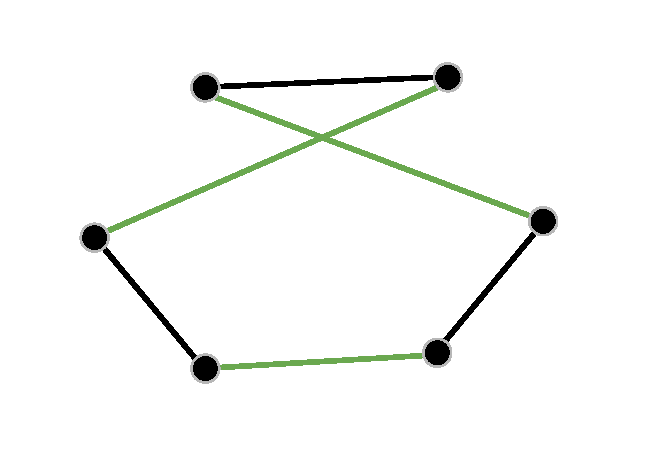
\includegraphics[width=\linewidth]{media/threeopt4.pdf}
    \caption{}
  \end{subfigure}
  \begin{subfigure}[b]{0.24\linewidth}
    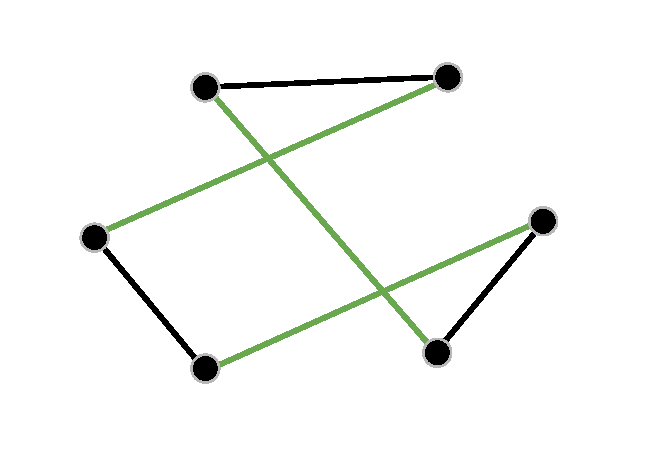
\includegraphics[width=\linewidth]{media/threeopt5.pdf}
     \caption{}
  \end{subfigure}
  \begin{subfigure}[b]{0.24\linewidth}
    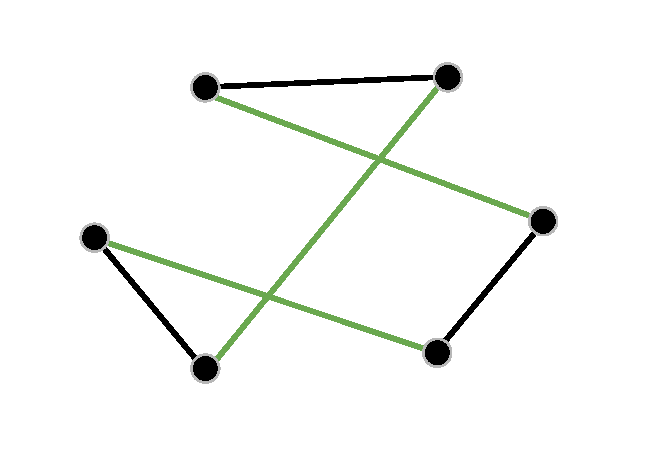
\includegraphics[width=\linewidth]{media/threeopt6.pdf}
    \caption{}
  \end{subfigure}
  \begin{subfigure}[b]{0.24\linewidth}
    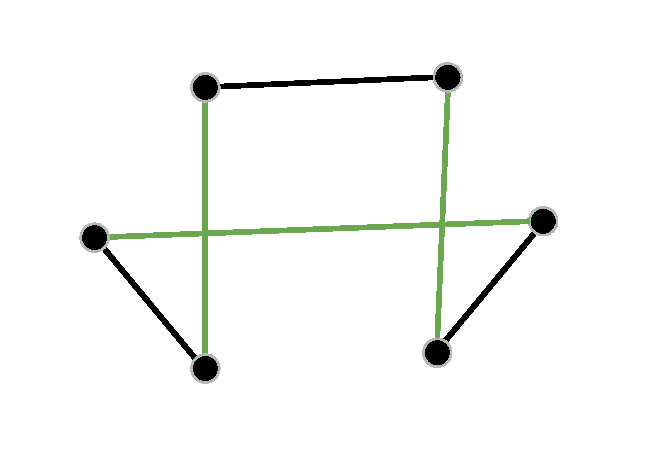
\includegraphics[width=\linewidth]{media/threeopt7.pdf}
    \caption{}
  \end{subfigure}
  \begin{subfigure}[b]{0.24\linewidth}
    \includegraphics[width=\linewidth]{media/threeopt8.pdf}
    \caption{}
  \end{subfigure}
  \caption{All the possible 3-OPT moves given a triad of edges.}
  \label{fig:threeopt}
\end{figure}
 
\noindent We also repeated the same experiment we did for the 2-OPT, so we run on different problems GRASP for 5 seconds and then 3-OPT on the result for other 5 second. The results are shown on Table \ref{tab:threeopt}. Again the dataset is small because the only goal was to show the power of this refinement algorithm and not to compare it with other techniques. Observing the table we can notice that the improve for the smaller problems is almost the same, or sometimes better than the one with 2-OPT, but more importantly we can notice that the algorithm scales bad with big problems due to the fact that it's cubic. In fact 5 seconds is a relatively small amount of time and in this short period the number of 3-OPT moves that the algorithm is able to perform is small so the improve is poor.

\begin{table}[h!]
	\begin{center}
		\begin{tabular}{l|c|c|c}
			\textbf{Instance} & \textbf{GRASP} & \textbf{3-OPT} & \textbf{Improve}	\\
			& (5 sec) & (5 sec) & \\
			\hline
			att48 & 42086 & 33588 & 20\% \\
			eil101 & 875 & 665 & 25\% \\
			ch130 & 9894 & 6373 & 35\% \\
			ch150 & 10503 & 6828 & 35\% \\
			a280 & 4588 & 3247 & 29\% \\
			lin318 & 75526 & 56496 & 25\% \\ 
			att532 & 153954 & 144295 & 6\% \\	
			pr1002 & 487157 & 481381 & 1\% \\
		\end{tabular}
		\caption{Values of the objective functions after running on each instance GRASP algorithm for 5 seconds and then 3-OPT for other 5 seconds.}
		\label{tab:threeopt}
	\end{center}
\end{table}

\newpage

\section{Metaheuristics}
A metaheuristic is a higher-level procedure or heuristic designed to find, generate, or select a heuristic (partial search algorithm) that may provide a sufficiently good solution to an optimization problem, especially with incomplete or imperfect information or limited computation capacity \footnote{R. Balamurugan; A.M. Natarajan; K. Premalatha (2015). "Stellar-Mass Black Hole Optimization for Biclustering Microarray Gene Expression Data". Applied Artificial Intelligence an International Journal.}


\subsection{Multi-start}
After performing a refinement technique, like 2-OPT, if the time limit is not reached, the algorithm stop on a local minima of the objective function. Of course at this point we want to escape from this local minima and search for a better one that hopefully is also the optimum. A possible solution is the multi-start approach, so each time we restart from the beginning, providing another initial solution and refining it. On each iteration, if the algorithm that provide the initial solution is well randomized (like GRASP) we will stop on a different local minima. So we can keep track of the best one and return it when the time limit for this procedure is reached.
The main problem of this technique is that is not very efficient because each time I restart all the information we obtained on the previous local minima is unused.
More powerful technique will be shown on the following subsections.

\subsection{Variable neighborhood search}
Variable neighborhood search (VNS) provide a simple yet powerful way to escape the local minima. Let's assume that we have completed the refinement using 2-OPT. At this point we can perform a random move with a bigger research radius, like a 3-OPT or a 5-OPT for example. Since this move is completely random, it will make the solution worse but it will also provide the ``kick" that we need to escape the local minima. Now we can restart with 2-OPT until a new minima is found (that could also be the optimum).\\
In synthesis, VNS, works with two phases that alternate continuously: an intensification  phase (2-OPT) where the algorithm move toward a minima and a diversification phase where VNS perform a k-OPT random move to exit from the minima.

\begin{algorithm}
	\caption{VNS}\label{VNS method}
	\hspace*{\algorithmicindent} \textbf{Input:} Admissible solution S \\
	\hspace*{\algorithmicindent} \textbf{Output:} Best solution found
    \begin{algorithmic}[1]
    		\State \textit{bestSolution $\leftarrow$ S}
		\While{! termination condition}
			\State bestMove $\leftarrow$ find best 2-OPT move of S
			\If{$\Delta($bestMove$) > 0$}
				\State S $\leftarrow$ perform bestMove
			\Else
				\State S $\leftarrow$ perform random k-OPT move
			\EndIf
			\If{cost$($S$)$ $<$ cost$($bestSolution$)$}
				\State bestSolution $\leftarrow S$
			\EndIf
		\EndWhile
		\State \textbf{return} bestSolution
    \end{algorithmic}
\end{algorithm}

\begin{figure}[h!]
\centering
	\includegraphics[scale=0.77]{media/vns_graph.pdf} \\
	\caption{Representation of an objective function during VNS and the ``kick" of a 5-OPT random move}
\end{figure}

\noindent On our implementation we use the technique showed in Figure \ref{fig:vns}. We select the edges to remove (that in our example are three) and then we reconnect the vertices in a specific way, so that the reversal of some edges to reconstruct the cycle (the one described in 5.2.1) is never required. In particular, because we can assign to the cycle a direction of travel, for each edge that we want to remove we can distinguish an initial vertex (the ones in red) and a final vertex (the ones in green). The idea is to always reconnect an initial vertex to a final vertex so the direction of travel is preserved. So for example we can start from the initial vertex of the first edge to remove and connect it to the final vertex of the second edge to remove. Then we pick the initial vertex of the second edge and we connect it to the final vertex of the third and so on, until the cycle is reconstructed. Of course this is valid for k edges, so on our implementation we can perform a k-opt random move, where k is establish at the beginning of the execution.

\begin{figure}[h!]
  \centering
  \begin{subfigure}[b]{0.49\linewidth}
    \includegraphics[width=\linewidth]{media/vnss12.pdf}
     \caption{}
  \end{subfigure}
  \begin{subfigure}[b]{0.49\linewidth}
    \includegraphics[width=\linewidth]{media/vnss22.pdf}
    \caption{}
  \end{subfigure}
  \begin{subfigure}[b]{0.49\linewidth}
    \includegraphics[width=\linewidth]{media/vnss32.pdf}
    \caption{}
  \end{subfigure}
  \caption{Passages for a k-OPT random move (In this case a 3-OPT move).}
  \label{fig:vns}
\end{figure}


\subsection{Tabu search}
Created by Fred W. Glover during the 80s, Tabu search provide an alternative procedure to VNS to escape from local minima. Let's assume that we have performed a refinement and we have reached a local minima, let's call this solution $x_k$. At this point, every 2-OPT move will make the objective function worse. So we choose and perform the least pejorative move, obtaining the solution $x_{k+1}$. Now, if we make another move following the 2-OPT rule, the algorithm will return to the solution $x_{k}$ by simply swapping again the edges used on the last step, cause this is the only move that improve the objective function. To avoid this, the idea is to insert these edges on a tabu list that is a list of edges that cannot be used for a 2-OPT move. This means that the move from $x_{k}$ to $x_{k+1}$ became forbidden. So we repeat this last step, performing the least pejorative move and each time inserting the edges used in the tabu list, until we reach a point where the objective function will return to improve. Of course we don't insert edges into the tabu list if the move is not pejorative. \\
To describe the algorithm we asserted that the tabu list is made of couples of edges, but this was only for a description purpose. In fact the general idea for this algorithm is that the tabu list can be made of any element that prevent to return back after a pejorative move. So for the TSP problem we can use, for example, couples of edges, a single edge or a single point. \\

\begin{algorithm}
	\caption{Tabu search}\label{TabuSearch method}
	\hspace*{\algorithmicindent} \textbf{Input:} Admissible solution S \\
	\hspace*{\algorithmicindent} \textbf{Output:} Best solution found
    \begin{algorithmic}[1]
    		\State \textit{bestSolution $\leftarrow$ S}
		\While{! termination condition}
			\If{tabuList is full}
				\State tabuList $\leftarrow$ empty list
			\EndIf
			\State bestMove $\leftarrow$ find best and not forbidden 2-OPT move of S
			\If{$\Delta($bestMove$) >$ 0}
				\State S $\leftarrow$ perform bestMove
			\Else
				\State S $\leftarrow$ perform bestMove
				\State tabuList $\leftarrow$ add(bestMove)
			\EndIf
			\If{cost$($S$)$ $<$ cost$($bestSolution$)$}
				\State bestSolution $\leftarrow S$
			\EndIf
		\EndWhile
		\State \textbf{return} bestSolution
    \end{algorithmic}
\end{algorithm}

\noindent The handle of the tabu list is very important and different strategies can have a big impact on the algorithm. Of course if we continue inserting element we will reach a point where there aren't possible moves. So we limit the size of the tabu list. The size is called tenure. When the list is full, the older element are removed.
The tenure is another parameter to set. A possible way to do this is to set a minimal and a maximal value and let the tenure oscillate among them during the algorithm. So we will have diversification phases when the tenure is big and there are lot of forbidden move and intensification phases when the tenure is small and the algorithm has lot of freedom. This is called reactive tabu search.
Another shrewdness is that if we encounter a move that is forbidden but that improves the incumbent, we will not perform that move but we will update the value of the incumbent in any case (Aspiration criterion).\\

\begin{figure}[h!]
\centering
	\includegraphics[scale=0.6]{media/tabuSearch1.png} \\
	\caption{Objective function and incumbent during the execution of tabu search}
\end{figure}

\noindent On our implementation we use a fixed-size tabu list, with the tenure that is a parameter decided by the user. The list records only one vertex involved in the move: so for example if we perform a pejorative move and we substitute the edges $v_{ab}$ and $v_{cd}$ with $v_{ac}$ and $v_{bd}$, only the vertex a is stored in the tabù list. When we find a good move, we check that all the 4 vertices involved are not in the tabu list, so even if we record only one point per move, this is sufficient to avoid to return back after a pejorative move. 
The check if a move is forbidden require a $O(k)$, where k is the tenure. So we perform this control only to moves that are better than the best move found until that moment (It's useless to check pejorative moves or moves that are not candidate to be selected as best move). \\
Finally we also implemented the aspiration criterion, so if a forbidden move leads to an improve of the incumbent, we keep that solution and we update the incumbent too.


\subsection{Simulated Annealing}
This metaheuristic algorithm take inspiration from the annealing technique in metallurgy that consist on heating the material and then cooling it in a controlled way. When the temperature of the materials is high, the atoms inside it it vibrates and move in a chaotic way. As the temperature decreases, the atoms reduce their state of agitation until a stable point is reached. \\
The simulated annealing works in a similar way. Let's establish a parameter, the temperature T, that initially has an high value that gradually reduce during the iterations of the algorithm. The algorithm starts from an already provided solution. On each iteration we perform a random 2-OPT (or 3-OPT) move that of course can be also pejorative. The fundamental idea is that the probability to accept the move is related to the temperature: when T is high, the system is chaotic and we accept with high probability all the random move. As the system get cooler we increase the probability to reject a bad move (so we increase the probability to perform a good move). When the temperature is close to 0, we only make meliorative moves until we reach a minima.\\
Considering the objective function, we have that, when T is high, the algorithm is randomly exploring solutions. Only when T became low the algorithm moves toward a minima that hopefully is the optimum.

\begin{figure}[h!]
\centering
	\includegraphics[scale=0.77]{media/sim_annealing.pdf} \\
	\caption{Example of the work of the simulated annealing. Note the initial random exploration with high temperature and the move toward the minima with a lower temperature.}
\end{figure}

\begin{algorithm}
	\caption{Simulated Annealing}\label{Annealing method}
	\hspace*{\algorithmicindent} \textbf{Input:} Admissible solution S \\
	\hspace*{\algorithmicindent} \textbf{Output:} Best solution found
    \begin{algorithmic}[1]
    		\State \textit{let p be the probability to accept a bad move}
    		\State \textit{let T be the temperature}
		\While{! termination condition}
			\State $\Delta \leftarrow$ random 2-OPT move
			\If{$\Delta > 0$}
				\State S $\leftarrow$ perform the move
			\Else 
				\State p $\leftarrow$ f$($T$)$
				\State r $\leftarrow$ random number $\in [0, 1)$
				\If{r $<$ p}
					\State S $\leftarrow$ perform the move
				\EndIf 
			\EndIf
			\If{temperature change condition}
				\State decrease T
			\EndIf
		\EndWhile
		\State \textbf{return} S
    \end{algorithmic}
\end{algorithm}

\noindent Of course the choose of the cooling schedule and the function that regulate the probability to accept a move with respect to the temperature are pivotal and can have a big impact on the performance of the algorithm itself. \\
On our implementation we followed the procedure showed in the paper %TODO add paper
that we are going to briefly explain.
Let X be the initial solution and Y a solution produced after a random 2-OPT move on x, let $f(X)$, $f(Y)$ be the cost respectively of X and Y, let $p_0$ be the initial probability. On each iteration, until the temperature list is full, generate a new Y. If $f(Y) > f(X)$ (pejorative move) compute a temperature with the following formula:
\begin{equation*}
t = \frac{-\vert f(y) - f(x) \vert}{\ln{(p_0)}}
\end{equation*}
otherwise, if $f(Y) < f(X)$, put X = Y and then compute t in the same way.
Now to describe the remaining part of our implementation let's consider N, that is a parameter decided by the user that indicate the maximum number of iteration where we use the same temperature. Let also i = 0, 1... N be a counter for those iteration. We start by extracting $T_{max}$ from the temperature list, this will be the temperature of the system for the next following N iteration. On each iteration we generate a random 2-OPT move: if it is meliorative the solution is simply updated. If it is pejorative we compute a probability $p_i$ defined as:
\begin{equation*}
p_i = \exp \Bigl( \frac{-(f(Y)-f(X))}{t_{max}} \Bigr)
\end{equation*}
then we generate a random number $r_i \in [0, 1)$ and if $r_i < p_i$ the move is accepted.
At this point, if we accept a bad move, we need to calculate another temperature $T_i$, defined as:
\begin{equation*}
T_i = \frac{-d_i}{p_i}
\end{equation*} 
where $d_i$ is the difference between $f(Y)$ and $f(X)$ on iteration i. We need also to keep in memory a counter c for each time we have performed a pejorative move. When we reach N iteration, we have to decrease the temperature: we compute the mean
\begin{equation*}
T_{mean} = \frac{1}{c} \sum T_i
\end{equation*}
and we substitute $T_{max}$ with $T_{mean}$. Since $T_i < T_{max}$ we have also that $T_{mean} < T_{max}$ so with the substitution we decrease the temperature. Now we pick another $T_{max}$ and we repeat the entire procedure until the algorithm terminate.



\subsection{Genetic Algorithm}
The genetic algorithm is inspired by the evolution theory, formulated by Charles Darwin during the $18^{th}$ century. 
The algorithm starts with a population where each individual that belong to the population itself is a solution to the problem, so in our case each individual is a solution for the TSP. Each individual has also a fitness that is defined as the cost of the solution. On each iteration (also called epoch), the individuals that have the highest fitness are removed from the population: maintaining the parallelism with the evolution theory we can say that the individuals that didn't adapt to the environment (high fitness) died.
On each iteration we have also that couples of individuals reproduce and the new elements substitute the ones that we have removed (so the population size remain constant). The children generated inherit characteristics from both their parents: a simple mechanism is just to pick part of the edges from one parent and the remaining from the other. Of course in this way the children is not a solution of the TSP problem cause some node may be visited more than once or may miss, so a repair function is required. In addition, at this point, a mutation function can be added: this mean that a children with probability x (that in general is low) can suffer a modify that hasn't any relation with its parents, like a random exchange of two vertices in the visit sequence. We can introduce this shrewdness to emulate in the algorithm the mutation mechanism that happens also in real life\\
After some iteration we have that the average fitness improve due to the fact that we remove bad solution and we generate new solution from the better ones. When the algorithm end, the champion of the population, that is the solution with the best fitness, is the final result. \\


\begin{algorithm}
	\caption{Genetic}\label{Genetic method}
	\hspace*{\algorithmicindent} \textbf{Input:} Population $P_t$ of solutions S, N number of new element per epoch \\
	\hspace*{\algorithmicindent} \textbf{Output:} Best individual of the population
    \begin{algorithmic}[1]
    		\State $\textit{t} \leftarrow 0$
    		\State $\textit{bestSolution}$
    		\State $\textit{fitnessList}$
    		\State fitnessList, bestSolution $\leftarrow$ computeFitness$(P_t)$ 
    		\While{! condition of termination}
    			\For{i $=$ 0, i $<$ N, i++}
    				\State removeElement$(P_t)$
    				\State update$($fitnessList$)$
    			\EndFor
    			\For{i $=$ 0, i $<$ N, i++}
    				\State S $\leftarrow$ generateNewChildren$(P_t)$
    				\State repair$($S$)$
    				\State fitnessList $\leftarrow$ add$($fitness$($S$))$
    				\If{fitness$($S$) < $ fitness$($bestSolution$)$}
    					\State bestSolution $\leftarrow S$
    				\EndIf
    			\EndFor
    			\State \textit{t} $\leftarrow$ t+1
    		\EndWhile
    		\State \textbf{return} bestSolution 
    \end{algorithmic}
\end{algorithm}


\noindent Our first implementation of this algorithm was pretty simple. We generated a population of a size decided by the user using the GRASP algorithm. We created a probability mass function (PMF) normalizing the sum of the fitness, so on each iteration we randomly chose the elements to remove based on that mass function. This means that during the firsts iterations, when all the individual have almost the same fitness, the element are almost randomly remove, while when the algorithm progress and there is a more evident difference between good and bad individuals, with high probability only the worst solutions are removed. The number of element to remove on each iteration (that is equal to the number of children to generate) is a parameter decided by the user. \\
To reproduce two elements we used the following technique: we chose a random number x between 0.3 and 0.7. Then we picked the first x visited node from one of the parent and the remaining from the other. At this point we used a repair function (Figure \ref{fig:genetic}) that remove all the points visited twice and insert the missing ones using the insertion algorithm described in 5.1.3. 

\begin{figure}[h!]
  \centering
  \begin{subfigure}[b]{0.49\linewidth}
    \includegraphics[width=\linewidth]{media/gene1.pdf}
     \caption{Non repaired children}
  \end{subfigure}
  \begin{subfigure}[b]{0.49\linewidth}
    \includegraphics[width=\linewidth]{media/gene2.pdf}
    \caption{Twice-visited vertices removal}
  \end{subfigure}
  \begin{subfigure}[b]{0.49\linewidth}
    \includegraphics[width=\linewidth]{media/gene3.pdf}
    \caption{Insertion of remaining element}
  \end{subfigure}
  \begin{subfigure}[b]{0.49\linewidth}
    \includegraphics[width=\linewidth]{media/gene4.pdf}
    \caption{Final result}
  \end{subfigure}
  \caption{Example of the steps of a repair function}
  \label{fig:genetic}
\end{figure}

\noindent The couples to reproduce are simply chosen at random from the population and we didn't implement any mechanism to control that same individual aren't choose more than once. We made this choice because on this algorithm the population have often big size, in general more than 10000 individuals, so the probability to pick the exactly same individuals more than once is very low.
After some run, plotting the average fitness and the best fitness, we could observe the 
expected behaviour (Figure \ref{fig:fitness}): the average fitness continuously decrease until it get closer to the best fitness (that improve only sometimes).  \\

\begin{figure}[h!]
\centering
	\includegraphics[scale=0.6]{media/fitnessPlot.png} \\
	\caption{Plot of the average fitness and best fitness during the execution of a genetic algorithm.}
	\label{fig:fitness}
\end{figure}

\noindent The problem of our implementation became evident after testing it on different instances: the solutions had lot of intersection (like the ones generated by the GRASP algorithm) that of course don't belong to the optimum. An example of this can be seen on Figure \ref{fig:geneticplot}. So we tried to introduce the 2-OPT someway inside the genetic. From this point, to distinguish the different versions of the genetic that we realized, we will call the implementation just described \textit{genetic 1}. \\
A possibility that we first considered but we immediately discarded was to just apply the 2-OPT algorithm on the final solution provided by the genetic. This didn't make lot of sense because we did a lot of effort to produce a result with the genetic and then we discard a consistent part of it using the 2-OPT: a simple GRASP plus 2-OPT would be more efficient.
Then we decided to add the 2-OPT to the repair function. So each children, after being repaired was also refined using the 2-OPT rule. Let's call this version \textit{genetic 2}. We immediately noticed a large reduction of the number of epochs executed in the same amount of time with respect to genetic 1. This is because the populations used in the genetic algorithm are large and even if 2-OPT is quite fast it has to be executed a lot of time. \\
Finally we tried an hybrid approach between genetic 1 and genetic 2: after the repair function the refinement is executed with a probability x decided by the user. With this version each epoch is faster than genetic 2 because the 2-OPT is executed less time, however the price of this is the introduction of another parameter that is the probability x.\\

\begin{figure}[h!]
\centering
	\includegraphics[scale=0.6]{media/genetic.png} \\
	\caption{Solution of the instance ch150 provided by our first implementation of the genetic. Note the big number of edge intersections.}
	\label{fig:geneticplot}
\end{figure}

\noindent We tested these three versions on the dataset to find which ones is the best. We establish a time limit of 10 minutes and a population size of 2000 elements with 200 new elements each epoch. The 2-OPT, when applied inside the repair function, has a time limit of one second. Note that we were forced to use a population with a limited size, in fact after few tests we discovered that it's very difficult to handle a big population (like 10000 or more elements) on a single machine, cause the algorithm became incredibly slow.
The Table \ref{tab:meta} report the final values of the objective functions obtained by each algorithm and the number of epoch that it was able to execute within the time limit. The first thing that we can notice, as expected, is that the introduction of the 2-OPT involves a big decrease of the epochs performed. However in both genetic 2 and 3 results are better, so even if we pay an increase of execution time for each epoch, the addition of the refinement is worth. This became more evident if we consider the performance profile (Figure \ref{fig:geneticPP}), where genetic 1 is far the worst algorithm. \\ 
Again, looking to the performance profile, genetic 2 seems to be the best, followed by genetic 3 that is slightly worse. However we chose genetic 3 as the winner of this first ``eliminatory phase" for the following reasons: first of all the difference in the performance profile is tiny and since the dataset used is quite small we cannot say with absolute certainty that genetic 2 is the best. Moreover if we perform a 2-OPT on each new element, we move away from the idea of the genetic, in fact each children has to pass through a repair function and then a refinement, so with high probability it will maintain very few elements of its parents. Finally we execute very few epochs with respect to genetic 1 and 3 and this is against the principle of the evolution of the population. So this is why we selected the third version of the algorithm to compete with the others metaheuristics.\\

\begin{table}[h!]
	\begin{center}
		\begin{tabular}{l|c|c|c|c|c|c}
			\textbf{Instance} & \textbf{Genetic 1} & \textbf{Epochs} & \textbf{Genetic 2} & \textbf{Epochs} & \textbf{Genetic 3} & \textbf{Epochs}\\
			& & & & & & \\
			\hline
			d657 & 58281 & 67 & 51628 & 6 & 51485 & 13 \\
			d1291 & 82270 & 9 & 60116 & 2 & 61857 & 3 \\
			fl417 & 13066 & 247 & 12040 & 3 & 12046 & 6 \\
			fl1400 & 29775 & 8 & 21836 & 2 & 21635 & 3 \\
			fl1577 & 37798 & 6 & 27996 & 1 & 30190 & 2 \\
			nrw1379 & 77437 & 7 & 65374 & 2 & 67865 & 3 \\
			p654 & 39289 & 67 & 34986 & 2 & 35216 & 5 \\
			pcb1173 & 83380 & 12 & 63693 & 2 & 63075 & 3 \\
			pcb3038 & 224091 & 1 & 217479 & 0 & 220982 & 0 \\
			pr1002 & 342579 & 19 & 278606 & 2 & 278935 & 4 \\
			pr2392 & 635460 & 1 & 566707 & 0 & 576564 & 0 \\
			rl1304 & 396680 & 9 & 316148 & 2 & 315956 & 3 \\
			rl1323 & 430922 & 8 & 325125 & 2 & 341412 & 3 \\
			rl1889 & 532907 & 3 & 486805 & 1 & 490274 & 1 \\
			u724 & 50800 & 48 & 44697 & 3 & 44857 & 7 \\
			u1060 & 309589 & 17 & 240649 & 2 & 241563 & 4 \\
			u2152 & 111343 & 1 & 98474 & 0 & 99573 & 0 \\
			u2319 & 316450 & 1 & 295777 & 0 & 297665 & 0 \\
			vm1084 & 326657 & 15 & 255282 & 2 & 258157 & 4 \\
			vm1748 & 502384 & 3 & 460075 & 1 & 480036 & 1 \\
		\end{tabular}
		\caption{Results of the eliminatory between the different versions of the genetic we implemented}
		\label{tab:meta}
	\end{center}
\end{table}

\begin{figure}[h!]
\centering
	\includegraphics[scale=0.9]{media/genetic.pdf} \\
	\caption{Performance profile of the three versions of the genetic algorithm we implemented}
	\label{fig:geneticPP}
\end{figure}

\noindent To conclude we noticed that the genetic algorithm is well suited to a distributed approach. On the big data domain, when, for example, we need to perform a clustering algorithm, a possible solution is to split the set of points into smaller chunks, and locate them on different machines that execute the operations on them independently. We can think to a similar solution for the genetic: we can divide a big population into smaller subset, assign each of them to a different machine (or a different core if we have only one computer) and apply the algorithm. Considering the parallelism with the evolution theory, we can think to this as if we have different populations living in different habitats. At this point it is also possible to introduce ``migrations" between different populations, this means that on each epoch we can randomly shuffle some elements between different subsets. 
So with this strategy we can run the genetic on a cluster, solving the problem of having to menage a big population and speeding up the execution of the algorithm.


\subsection{Final comparison between metaheuristics}

\begin{figure}[h!]
\centering
	\includegraphics[scale=0.9]{media/metaheuristics.pdf} \\
	\caption{Performance profile of the metaheuristics}
	\label{fig:metaheuristics}
\end{figure}

On Figure \ref{fig:metaheuristics} it is possible to see the performance profile of all the metaheuristics we analyzed in this section. We tested each algorithm on the usual dataset with a time limit of 30 minute per instance (all the other details about the experiments are report on section 5.4). The parameter we used are the following:

\begin{itemize}
	\item \textbf{Multi start}: no parameter except for time limit.
	\item \textbf{VNS}: 5-OPT random move for the kick.
	\item \textbf{Tabu search}: tenure equals to 40\% of the instance size.
	\item \textbf{Simulated annealing}: temperature list of 5000 elements, 1000 iteration with the same temperature.
	\item \textbf{Genetic}: population size of 2000, 200 new elements per epoch. 
\end{itemize}

\noindent The first thing we can notice is that the VNS has the best performance. Of course our dataset is quite small, so we cannot say with absolute certainty that VNS is in absolute the best algorithm. However our results are aligned with the ones we saw during the course and the ones obtained by other students, so we can conclude that VNS is a very good heuristic solution for the TSP. \\
Another thing we can notice are the poor performance of the genetic. This result was expected due to the fact we were forced to use small populations and to introduce the 2-OPT at the expense of the number of epoch for each run. \\
Finally, noteworthy is the simulates annealing that seems to have very good performance.


\chapter{Conclusions}
In conclusion let's summarize the results we obtained. Considering the compact models, we have that the flow based formulations, in particular flow 1 and flow 2, perform better than the MTZ and the time based formulations. Looking to the Performance profile we can conclude that flow 1 is the best compact model.
Moving to the exact algorithms, here we use the base TSP model, with different strategies to add the subtour eliminator constraints during (callbacks) or after (loop method) the execution of CPLEX. In general we have that these type of algorithms work better than a simple compact model. Again looking to the performance profile we can establish that the combination of the UserCut and Heuristic Callbacks based on the Generic Callback is the best strategy.
In the matheuristic chapter we analyze some heuristic solutions that are based on CPLEX and we reach the conclusion that hard fixing is the best matheuristic.
Finally in the stand-alone heuristics chapter we explore several strategies that don't provide an exact solution and are independent from CPLEX. We conclude that VNS is probably the best performing heuristic and simulated annealing and tabu search can be good solutions too. \\

\noindent So if the goal is to resolve a relatively small instance of the TSP or we have big computational power and lots of time, we suggest to use CPLEX with UserCut and Heuristic Callbacks based on the Generic Callback. Otherwise if we have to resolve a big instance or we are not interested to obtain the exact solution and we have a time limit that is very important to respect we suggest VNS. 


\bibliographystyle{ieeetr}
\bibliography{biblio}


\chapter{Results Tables}

In this chapter we report the time measurements of all the algorithms that we have implemented and described in this report. For Callback methods we have also reported the number of nodes solved to compute the problem to optimum.

\section{Compact Models} 
In this section we report the time measurements of the Compact Models with their relative seed and algorithm.

\begin{center}
\begin{longtable}{llrrrr}
\caption{\textbf{\large Compact Models}} \label{tab:Loop} \\

\hline \multicolumn{1}{l}{\textbf{Instance}} & \multicolumn{1}{l}{\textbf{Seed}} & \multicolumn{1}{r}{\textbf{MTZ}}& \multicolumn{1}{r}{\textbf{Flow 1}} & \multicolumn{1}{r}{\textbf{Flow 2}} & \multicolumn{1}{r}{\textbf{Flow 3}}  \\ \hline
\endfirsthead

\multicolumn{6}{c}%
{{\bfseries \tablename\ \thetable{} -- continued from previous page}} \\
\hline \multicolumn{1}{l}{\textbf{Instance}} & \multicolumn{1}{l}{\textbf{Seed}} & \multicolumn{1}{r}{\textbf{MTZ}}& \multicolumn{1}{r}{\textbf{Flow 1}} & \multicolumn{1}{r}{\textbf{Flow 2}} & \multicolumn{1}{r}{\textbf{Flow 3}}  \\ \hline
\endhead

\hline \multicolumn{6}{r}{{Continued on next page}} \\ \hline
\endfoot

\hline \hline
\endlastfoot

ulysses22 & 23 & 516.927 & 0.343 & 0.359 & 3.348 \\
att48 & 23 & 3.855 & 1.327 & 1.791 & 186.627 \\
ulysses16 & 23 & 3.938 & 0.452 & 0.142 & 0.734 \\
st70 & 23 & 1147.487 & 137.717 & 192.168 & 8418.164 \\
pr76 & 23 & 77.406 & 100.940 & 284.219 & 2667.292 \\
eil76 & 23 & 20.430 & 183.920 & 130.450 & 18915.042 \\
eil51 & 23 & 3.328 & 32.711 & 32.251 & 1659.084 \\
berlin52 & 23 & 30.065 & 35.455 & 73.215 & 4405.665 \\
burma14 & 23 & 0.218 & 0.110 & 0.114 & 0.193 \\

ulysses22 & 2123 & 527.003 & 0.390 & 0.907 & 3.498 \\
att48 & 2123 & 5.303 & 1.793 & 1.808 & 194.977 \\
ulysses16 & 2123 & 3.114 & 0.106 & 0.286 & 0.740 \\
st70 & 2123 & 1356.786 & 230.846 & 122.904 & 4243.212 \\
pr76 & 2123 & 108.559 & 112.697 & 190.324 & 2616.969 \\
eil76 & 2123 & 15.946 & 282.910 & 353.393 & 14471.835 \\
eil51 & 2123 & 2.289 & 7.554 & 46.835 & 6745.074 \\
berlin52 & 2123 & 92.319 & 12.675 & 83.720 & 4713.600 \\
burma14 & 2123 & 0.151 & 0.131 & 0.110 & 0.216 \\

ulysses22 & 48399 & 768.739 & 0.253 & 0.496 & 3.308\\
att48 & 48399 & 4.348 & 1.547 & 1.453 & 197.239 \\
ulysses16 & 48399 & 3.141 & 0.227 & 0.250 & 0.665 \\
st70 & 48399 & 1356.786 & 257.183 & 265.412 & 4616.888 \\
pr76 & 48399 & 71.636 & 76.051 & 234.136 & 2707.392 \\
eil76 & 48399 & 8.915 & 230.493 & 421.678 & 24884.819 \\
eil51 & 48399 & 0.888 & 15.096 & 60.214 & 1033.519 \\
berlin52 & 48399 & 46.524 & 18.031 & 69.704 & 7270.184 \\
burma14 & 48399 & 0.149 & 0.212 & 0.078 & 0.216 \\

\end{longtable}
\end{center}

\newpage
\section{Exact Algorithms} 
In this section we report the time measurements (in seconds) of the Exact Algorithms with their relative seed and algorithm.

\begin{center}
\begin{longtable}{llrr}
\caption{\textbf{\large Loop Methods}} \label{tab:Loop} \\

\hline \multicolumn{1}{l}{\textbf{Instance}} & \multicolumn{1}{l}{\textbf{Seed}} & \multicolumn{1}{r}{\textbf{Simple Loop}}& \multicolumn{1}{r}{\textbf{Heuristic Loop}} \\ \hline
\endfirsthead

\multicolumn{4}{c}%
{{\bfseries \tablename\ \thetable{} -- continued from previous page}} \\
\hline \multicolumn{1}{l}{\textbf{Instance}} & \multicolumn{1}{l}{\textbf{Seed}} & \multicolumn{1}{r}{\textbf{Simple Loop}}& \multicolumn{1}{r}{\textbf{Heuristic Loop}} \\ \hline
\endhead

\hline \multicolumn{4}{r}{{Continued on next page}} \\ \hline
\endfoot

\hline \hline
\endlastfoot

			a280 & 201909284 & 29.781 & 32.546 \\
			att48 & 201909284 & 0.681 & 0.594  \\
			att532 & 201909284 &  663.910 & 719.934\\
			berlin52 & 201909284 & 0.095 & 0.063  \\
			bier127 & 201909284 & 4.407 & 5.622 \\
			ch130 & 201909284 & 5.103 & 5.557  \\
			ch150 & 201909284 & 11.128 & 15.697  \\
			d198 & 201909284 & 72.351 & 69.021   \\
			gil262 & 201909284 & 55.548 & 49.800   \\
			kroA100 & 201909284 & 4.419 & 4.651   \\
			kroA150 & 201909284 & 23.498 & 16.290  \\
			kroA200 & 201909284 & 64.854 & 82.079   \\
			kroB100 & 201909284 & 7.698 & 7.828  \\
			kroB150 & 201909284 & 34.584 & 31.630  \\
			kroB200 & 201909284 & 22.810 & 19.158  \\
			kroC100 & 201909284 & 4.956 & 3.526   \\
			kroD100 & 201909284 & 4.964 & 4.677  \\
			kroE100 & 201909284 & 4.540 & 4.475  \\
			lin105 & 201909284 & 3.567 & 4.633   \\
			lin318 & 201909284 & 97.536 &110.049  \\
			pr226 & 201909284 & 197.544 & 260.199 \\
			rat195 & 201909284 & 69.132 & 47.261  \\
			pr76 & 201909284 & 9.330 & 8.509 \\
			pr107 & 201909284 & 0.631 & 2.172  \\
			pr124 & 201909284 & 20.794 & 23.092 \\
			pr136 & 201909284 & 5.627 & 6.156  \\
			tsp225 & 201909284 & 32.324 & 29.078  \\
			u159 & 201909284 & 7.316 & 7.618   \\
			rat99 & 201909284 & 2.413 & 2.727  \\
			rd400 & 201909284 & 305.766 & 456.781  \\
			
a280 & 19 & 29.235 & 24.520 \\
att48  & 19 & 0.593 & 0.671 \\
att532  & 19 & 734.706&756.783\\
berlin52  & 19 & 0.097& 0.065\\
bier127  & 19 & 4.456& 5.910\\
ch130  & 19 & 5.183& 6.728\\
ch150  & 19 & 10.200& 17.139\\
d198  & 19 & 65.949;&70.533\\
gil262  & 19 & 54.885&42.880\\
kroA100  & 19 & 4.190&4.722\\
kroA150  & 19 & 25.094&17.489\\
kroA200  & 19 & 82.620& 84.170\\
kroB100  & 19 & 8.183&7.517\\
kroB150 & 19 & 33.041& 29.433\\
kroB200  & 19 & 28.127& 12.029\\
kroC100  & 19 & 4.825& 3.915\\
kroD100 & 19 & 5.098& 4.810\\
kroE100  & 19 & 4.362& 4.274\\
lin105  & 19 & 2.935& 4.384\\
lin318  & 19 & 95.144& 103.283\\
pr226  & 19 & 375.243& 245.419\\
rat195  & 19 & 63.654& 72.675\\
pr76  & 19 & 8.932& 9.417\\
pr107  & 19 & 0.578 & 3.075\\
pr124  & 19 & 19.232 & 19.579\\
pr136  & 19 & 5.519& 7.685\\
tsp225  & 19 & 32.647& 27.622\\
u159  & 19 & 7.472& 8.665\\
rat99  & 19 & 1.829& 3.217\\
rd400  & 19 & 372.713& 321.477\\
a280 & 190796 & 26.739& 25.632\\
att48  & 190796 & 0.632& 0.611\\
att532  & 190796 &723.908& 777.047\\
berlin52  & 190796 & 0.092& 0.166\\
bier127  & 190796 & 4.320& 5.399\\
ch130  & 190796 & 5.034& 7.076\\
ch150  & 190796 & 12.824& 18.325\\
d198  & 190796 & 63.516& 52.336\\
gil262  & 190796 & 52.419& 43.887\\
kroA100  & 190796 & 4.025& 4.328\\
kroA150  & 190796 & 23.075& 17.093\\
kroA200  & 190796 & 84.148& 78.703\\
kroB100  & 190796 & 7.607& 7.928\\
kroB150  & 190796 & 34.306& 33.014\\
kroB200  & 190796 & 24.217& 13.384\\
kroC100  & 190796 & 4.926& 3.206\\
kroD100  & 190796 & 5.197& 4.223\\
kroE100  & 190796 & 5.123& 4.568\\
lin105  & 190796 & 3.519& 2.837\\
lin318  & 190796 & 99.489& 91.392\\
pr226  & 190796  & 181.923& 555.863\\
rat195  & 190796 & 59.865& 50.482\\
pr76  & 190796 &10.316& 8.644\\
pr107  & 190796 & 0.555& 2.458\\
pr124  & 190796 & 21.904& 23.429\\
pr136  & 190796 & 6.314& 6.603\\
tsp225  & 190796 & 32.958& 32.733\\
u159  & 190796 & 7.975& 6.037\\
rat99  & 190796 & 2.170& 2.127\\
rd400  & 190796 & 336.298& 391.179\\
a280  & 19071996 & 31.560& 22.689\\
att48  & 19071996 & 0.668& 0.679\\
att532  & 19071996 & 656.097& 696.500\\
berlin52  & 19071996 & 0.103 & 0.086\\
bier127  & 19071996 & 4.610& 4.364\\
ch130  & 19071996 & 4.844& 6.604\\
ch150  & 19071996 & 10.942& 15.347\\
d198  & 19071996 & 71.141& 67.801\\
gil262  & 19071996 &61.853;&45.738\\
kroA100  & 19071996 & 4.449& 4.557\\
kroA150  & 19071996 &27.511& 15.670\\
kroA200  & 19071996 & 59.241& 81.205\\
kroB100  & 19071996 & 8.467& 7.117\\
kroB150  & 19071996 & 37.819& 27.418\\
kroB200  & 19071996 & 23.213& 18.620\\
kroC100  & 19071996 & 4.877& 3.207\\
kroD100  & 19071996 & 5.093& 4.278\\
kroE100  & 19071996 & 4.483& 3.851\\
lin105  & 19071996 & 3.633& 4.231\\
lin318  & 19071996 & 95.643& 99.793\\
pr226  & 19071996 & 156.506& 146.272\\
rat195  & 19071996 & 67.494& 63.071\\
pr76  & 19071996 & 8.173& 9.800\\
pr107  & 19071996 & 0.552& 1.506\\
pr124  & 19071996 & 22.828& 18.270\\
pr136  & 19071996 & 6.206& 8.585\\
tsp225  & 19071996 & 34.639& 32.599\\
u159  & 19071996 & 7.453& 7.642\\
rat99  & 19071996 & 2.339&2.207\\
rd400  & 19071996 & 337.442& 374.722\\
\end{longtable}
\end{center}


\begin{center}
\begin{longtable}{llrrr}
\caption{\textbf{\large Legacy Callbacks}} \label{tab:Loop} \\

\hline \multicolumn{1}{l}{\textbf{Instance}} & \multicolumn{1}{l}{\textbf{Seed}} & \multicolumn{1}{r}{\textbf{Lazy}}& \multicolumn{1}{r}{\textbf{UserCut}} & \multicolumn{1}{r}{\textbf{Heuristic}} \\ \hline
\endfirsthead

\multicolumn{5}{c}%
{{\bfseries \tablename\ \thetable{} -- continued from previous page}} \\
\hline \multicolumn{1}{l}{\textbf{Instance}} & \multicolumn{1}{l}{\textbf{Seed}} & \multicolumn{1}{r}{\textbf{Lazy}}& \multicolumn{1}{r}{\textbf{UserCut}} & \multicolumn{1}{r}{\textbf{Heuristic}} \\ \hline
\endhead

\hline \multicolumn{5}{r}{{Continued on next page}} \\ \hline
\endfoot

\hline \hline
\endlastfoot

a280 & 201909284 & 6.229 & 3.674 & 3.671\\
att48 & 201909284 & 0.095 & 0.069 & 0.057\\
att532 &19071996 & 3532.022 & 3511.272 & 3504.440\\
berlin52 &19071996 & 0.028 & 0.029 & 0.029\\
bier127 &19071996 & 1.219 & 0.592 & 0.626\\
ch130 &19071996 & 1.389 & 0.990 & 0.915\\
ch150 &19071996 & 5.351 & 2.396 & 1.571\\
d198 &19071996 & 40.486 & 4.199 & 4.336\\
gil262 &19071996 & 163.289 & 21.162 & 23.463\\
kroA100 &19071996 & 1.183 & 0.758 & 0.678\\
kroA150 &19071996 & 6.082 & 3.761 & 4.292\\
kroA200 &19071996 & 209.747 & 41.006 & 78.697\\
kroB100 &19071996 & 1.614 & 0.799 & 0.647\\
kroB150 &19071996 & 20.045 & 9.197 & 8.712\\
kroB200 &19071996 & 22.930 & 4.129 & 3.325\\
kroC100 &19071996 & 0.804 & 0.670 & 0.666\\
kroD100 &19071996 & 1.064 & 0.794 & 0.632\\
kroE100 &19071996 & 3.159 & 1.957 & 3.083\\
lin105 &19071996 & 0.497 & 0.210 & 0.218\\
lin318 &19071996 & 103.086 & 22.930 & 26.731\\
pr226 &19071996 & 27.445 & 4.292 & 4.380\\
rat195 &19071996 & 43.155 & 21.471 & 14.749\\
pr76 &19071996 & 14.067 & 11.805 & 4.295\\
pr107 &19071996 & 0.068 & 0.052 & 0.087\\
pr124 &19071996 & 2.134 & 1.826 & 1.614\\
pr136 &19071996 & 1.226 & 1.533 & 1.563\\
tsp225 &19071996 & 40.637 & 4.016 & 2.634\\
u159  &19071996 & 1.880 & 0.761 & 0.926\\
rat99 &19071996 & 0.488 & 0.350 & 0.369\\
rd400 &19071996 & 3551.366 & 461.552 & 564.476\\
a280 & 19 & 8.130 & 4.269 & 4.317\\
att48  & 19 & 0.089 & 0.071 & 0.056\\
att532  & 19 & 3535.718 & 1061.775 & 1233.420\\
berlin52  & 19 & 0.028 & 0.028 & 0.026\\
bier127  & 19 & 0.896 & 0.785 & 0.663\\
ch130  & 19 & 1.438 & 1.083 & 1.128\\
ch150  & 19 & 7.742 & 3.105 & 2.110\\
d198  & 19 & 23.188 & 6.341 & 4.156\\
gil262  & 19 & 116.108 & 44.069 & 34.565\\
kroA100  & 19 & 1.222 & 0.869 & 0.612\\
kroA150  & 19 & 8.917 & 3.338 & 3.783\\
kroA200  & 19 & 110.787 & 36.201 & 36.140\\
kroB100  & 19 & 2.114 & 0.711 & 0.464\\
kroB150 & 19 & 28.851 & 6.063 & 7.115\\
kroB200  & 19 & 32.032 & 4.254 & 6.101\\
kroC100  & 19 & 0.844 & 0.722 & 0.656\\
kroD100  & 19 & 0.983 & 0.770 & 0.789\\
kroE100  & 19 & 2.466 & 1.265 & 1.430\\
lin105  & 19 & 0.419 & 0.212 & 0.236\\
lin318  & 19 & 198.618 & 23.924 & 22.958\\
pr226  & 19 & 18.191 & 4.840 & 4.886\\
rat195  & 19 & 51.779 & 11.243 & 12.493\\
pr76  & 19 & 13.690 & 11.829 & 3.883\\
pr107  & 19 & 0.052 & 0.053 & 0.088\\
pr124  & 19 & 7.439 & 2.004 & 1.831\\
pr136  & 19 & 1.416 & 1.803 & 1.726\\
tsp225  & 19 & 29.004 & 4.494 & 3.006\\
u159  & 19 & 2.805 & 0.844 & 1.090\\
rat99  & 19 & 0.460 & 0.470 & 0.302\\
rd400  & 19 & 3565.286 & 601.292 & 704.836\\
a280 & 190796 & 10.591 & 4.896 & 5.036\\
att48  & 190796 & 0.091 & 0.070 & 0.059\\
att532  & 190796 & 3550.588 & 639.059 & 1448.989\\
berlin52  & 190796 & 0.031 & 0.031 & 0.028\\
bier127  & 190796 & 0.994 & 0.590 & 0.626\\
ch130  & 190796 & 2.110 & 1.267 & 0.924\\
ch150  & 190796 & 6.682 & 1.663 & 1.957\\
d198  & 190796 & 19.916 & 5.745 & 5.395\\
gil262  & 190796 & 231.023 & 13.520 & 22.168\\
kroA100  & 190796 & 1.269 & 0.751 & 0.739\\
kroA150  & 190796 & 10.130 & 3.806 & 2.339\\
kroA200  & 190796 & 243.669 & 96.150 & 62.074\\
kroB100  & 190796 & 1.104 & 0.930 & 0.947\\
kroB150  & 190796 & 23.558 & 6.720 & 6.849\\
kroB200  & 190796 & 79.954 & 5.045 & 4.684\\
kroC100  & 190796 & 0.998 & 0.645 & 0.657\\
kroD100  & 190796 & 1.026 & 0.727 & 0.731\\
kroE100  & 190796 & 2.600 & 1.667 & 1.776\\
lin105  & 190796 & 0.573 & 0.214 & 0.213\\
lin318  & 190796 & 211.935 & 48.083 & 17.926\\
pr226  & 190796 & 19.142 & 5.849 & 5.889\\
rat195  & 190796 & 43.599 & 15.382 & 15.497\\
pr76  & 190796 & 12.072 & 8.309 & 4.701\\
pr107  & 190796 & 0.052 & 0.052 & 0.088\\
pr124  & 190796 & 2.698 & 2.273 & 2.232\\
pr136  & 190796 & 2.104 & 1.412 & 1.259\\
tsp225  & 190796 & 13.332 & 5.804 & 2.825\\
u159  & 190796 & 2.792 & 0.754 & 0.896\\
rat99  & 190796 & 0.639 & 0.381 & 0.427\\
rd400  & 190796 & 3562.556 & 312.888 & 249.195\\
a280  & 19071996 & 15.257 & 5.946 & 5.931\\
att48  & 19071996 & 0.093 & 0.070 & 0.056\\
att532  & 19071996 & 3547.388 & 2244.815 & 3504.358\\
berlin52  & 19071996 & 0.031 & 0.030 & 0.028\\
bier127  & 19071996 & 0.896 & 0.610 & 0.627\\
ch130  & 19071996 & 1.651 & 1.051 & 0.949\\
ch150  & 19071996 & 6.329 & 2.499 & 2.583\\
d198  & 19071996 & 55.018 & 5.765 & 5.581\\
gil262  & 19071996 & 168.740 & 34.147 & 32.721\\
kroA100  & 19071996 & 1.515 & 0.756 & 0.679\\
kroA150  & 19071996 & 8.992 & 4.686 & 3.257\\
kroA200  & 19071996 & 453.677 & 98.514 & 112.663\\
kroB100  & 19071996 & 1.847 & 0.760 & 0.710\\
kroB150  & 19071996 & 18.980 & 7.197 & 10.153\\
kroB200  & 19071996 & 16.922 & 4.777 & 4.853\\
kroC100  & 19071996 & 0.853 & 0.658 & 0.682\\
kroD100  & 19071996 & 0.627 & 0.658 & 0.551\\
kroE100  & 19071996 & 2.643 & 1.991 & 2.032\\
lin105  & 19071996 & 0.532 & 0.256 & 0.219\\
lin318  & 19071996 & 93.532 & 33.001 & 21.742\\
pr226  & 19071996 & 16.314 & 4.834 & 4.878\\
rat195  & 19071996 & 29.843 & 13.269 & 12.237\\
pr76  & 19071996 & 19.724 & 7.595 & 4.206\\
pr107  & 19071996 & 0.052 & 0.049 & 0.088\\
pr124  & 19071996 & 3.873 & 1.828 & 1.899\\
pr136  & 19071996 & 1.953 & 1.352 & 1.729\\
tsp225  & 19071996 & 11.742 & 4.704 & 4.759\\
u159  & 19071996 & 2.977 & 0.769 & 0.808\\
rat99  & 19071996 & 0.496 & 0.352 & 0.353\\
rd400  & 19071996 & 3563.643 & 223.105 & 408.701\\
\end{longtable}
\end{center}


\begin{center}
\begin{longtable}{llrrr}
\caption{\textbf{\large Generic Callbacks}} \label{tab:Loop} \\

\hline \multicolumn{1}{l}{\textbf{Instance}} & \multicolumn{1}{l}{\textbf{Seed}} & \multicolumn{1}{r}{\textbf{Lazy}}& \multicolumn{1}{r}{\textbf{UserCut}} & \multicolumn{1}{r}{\textbf{Heuristic}} \\ \hline
\endfirsthead

\multicolumn{5}{c}%
{{\bfseries \tablename\ \thetable{} -- continued from previous page}} \\
\hline \multicolumn{1}{l}{\textbf{Instance}} & \multicolumn{1}{l}{\textbf{Seed}} & \multicolumn{1}{r}{\textbf{Lazy}}& \multicolumn{1}{r}{\textbf{UserCut}} & \multicolumn{1}{r}{\textbf{Heuristic}} \\ \hline
\endhead

\hline \multicolumn{5}{r}{{Continued on next page}} \\ \hline
\endfoot

\hline \hline
\endlastfoot

a280 & 201909284 & 12.946 & 12.593 & 14.801\\
att48 & 201909284 & 0.184 & 0.187 & 0.209\\
att532 & 201909284 & 2446.941 & 639.188 & 460.378\\
berlin52 & 201909284 & 0.077 & 0.096 & 0.080\\
bier127 & 201909284 & 3.442 & 1.739 & 1.149\\
ch130 & 201909284 & 4.504 & 4.221 & 1.673\\
ch150 & 201909284 & 9.392 & 6.332 & 6.024\\
d198 & 201909284 & 29.695 & 12.840 & 11.985\\
gil262 & 201909284 & 64.250 & 42.878 & 25.663\\
kroA100 & 201909284 & 2.967 & 2.888 & 0.898\\
kroA150 & 201909284 & 10.574 & 6.380 & 9.067\\
kroA200 & 201909284 & 69.231 & 25.079 & 28.455\\
kroB100 & 201909284 & 5.871 & 2.644 & 1.980\\
kroB150 & 201909284 & 15.901 & 6.044 & 6.368\\
kroB200 & 201909284 & 26.611 & 11.157 & 14.564\\
kroC100 & 201909284 & 1.204 & 1.121 & 0.981\\
kroD100 & 201909284 & 1.418 & 1.694 & 1.141\\
kroE100 & 201909284 & 4.858 & 3.181 & 1.501\\
lin105 & 201909284 & 1.444 & 0.801 & 0.648\\
lin318 & 201909284 & 67.349 & 25.349 & 29.021\\
pr226 & 201909284 & 29.891 & 18.124 & 15.023\\
rat195 & 201909284 & 32.835 & 33.280 & 12.177\\
pr76 & 201909284 & 6.359 & 6.835 & 2.957\\
pr107 & 201909284 & 0.126 & 0.086 & 0.136\\
pr124 & 201909284 & 4.793 & 2.574 & 2.315\\
pr136 & 201909284 & 2.673 & 1.776 & 1.540\\
tsp225 & 201909284 & 21.783 & 13.709 & 9.678\\
u159 & 201909284 & 4.659 & 1.953 & 2.395\\
rat99 & 201909284 & 0.579 & 0.585 & 0.586\\
rd400 & 201909284 & 197.624 & 131.576 & 113.149\\
a280 & 19 & 20.864 & 15.620 & 9.475\\
att48  & 19 & 0.174 & 0.181 & 0.145\\
att532  & 19 & 2744.552 & 534.519 & 281.131\\
berlin52  & 19 & 0.073 & 0.072 & 0.086\\
bier127  & 19 & 3.684 & 2.627 & 1.267\\
ch130  & 19 & 5.851 & 4.489 & 1.615\\
ch150  & 19 & 12.946 & 8.178 & 4.030\\
d198  & 19 & 31.508 & 13.839 & 10.980\\
gil262  & 19 & 64.308 & 34.720 & 31.280\\
kroA100  & 19 & 1.984 & 1.401 & 0.906\\
kroA150  & 19 & 12.968 & 9.416 & 5.820\\
kroA200  & 19 & 67.595 & 33.454 & 17.821\\
kroB100  & 19 & 3.784 & 2.542 & 1.878\\
kroB150 & 19 & 18.894 & 13.727 & 4.816\\
kroB200  & 19 & 16.304 & 12.599 & 8.692\\
kroC100  & 19 & 2.578 & 1.514 & 1.061\\
kroD100  & 19 & 1.531 & 1.163 & 1.328\\
kroE100  & 19 & 4.791 & 3.421 & 1.445\\
lin105  & 19 & 0.657 & 0.601 & 0.761\\
lin318  & 19 & 55.896 & 25.346 & 21.318\\
pr226  & 19 & 28.894 & 15.489 & 15.526\\
rat195  & 19 & 43.827 & 33.000 & 15.290\\
pr76  & 19 & 6.057 & 8.389 & 4.631\\
pr107  & 19 & 0.086 & 0.087 & 0.137\\
pr124  & 19 & 6.104 & 3.381 & 4.564\\
pr136  & 19 & 2.411 & 2.316 & 2.354\\
tsp225  & 19 & 14.538 & 12.006 & 9.069\\
u159  & 19 & 5.335 & 2.706 & 2.917\\
rat99  & 19 & 0.610 & 0.592 & 0.598\\
rd400  & 19 & 228.320 & 117.198 & 96.235\\
a280 & 190796 & 16.525 & 22.052 & 16.995\\
att48  & 190796 & 0.159 & 0.163 & 0.133\\
att532  & 190796 & 2196.201 & 583.651 & 404.120\\
berlin52 & 190796 & 0.067 & 0.068 & 0.069\\
bier127  & 190796 & 3.782 & 1.934 & 1.298\\
ch130  & 190796 & 4.024 & 3.708 & 1.990\\
ch150  & 190796 & 12.687 & 4.771 & 3.670\\
d198  & 190796 & 31.920 & 9.793 & 13.984\\
gil262  & 190796 & 47.178 & 56.418 & 32.368\\
kroA100  & 190796 & 2.773 & 2.263 & 1.023\\
kroA150  & 190796 & 10.338 & 11.541 & 6.809\\
kroA200  & 190796 & 21.538 & 52.614 & 22.347\\
kroB100  & 190796 & 2.759 & 2.189 & 1.679\\
kroB150  & 190796 & 12.962 & 14.925 & 4.931\\
kroB200  & 190796 & 12.705 & 13.328 & 11.764\\
kroC100  & 190796 & 2.144 & 1.681 & 0.946\\
kroD100  & 190796 & 1.527 & 1.420 & 1.133\\
kroE100  & 190796 & 3.471 & 4.130 & 1.416\\
lin105  & 190796 & 0.926 & 0.647 & 0.722\\
lin318  & 190796 & 176.928 & 30.363 & 33.881\\
pr226  & 190796 & 113.334 & 16.882 & 18.258\\
rat195  & 190796 & 30.761 & 19.633 & 16.996\\
pr76  & 190796 & 6.822 & 9.637 & 4.680\\
pr107  & 190796 & 0.086 & 0.088 & 0.138\\
pr124  & 190796 & 9.535 & 2.334 & 4.686\\
pr136  & 190796 & 2.576 & 3.237 & 2.173\\
tsp225  & 190796 & 15.866 & 13.499 & 7.800\\
u159  & 190796 & 5.308 & 2.526 & 1.916\\
rat99  & 190796 & 0.505 & 0.507 & 0.569\\
rd400  & 190796 & 186.584 & 231.009 & 81.896\\
a280  & 19071996 & 15.386 & 15.735 & 17.806\\
att48  & 19071996 & 0.160 & 0.164 & 0.134\\
att532  & 19071996 & 1077.461 & 1191.602 & 303.004\\
berlin52  & 19071996 & 0.073 & 0.073 & 0.085\\
bier127  & 19071996 & 4.199 & 1.947 & 1.435\\
ch130  & 19071996 & 2.771 & 2.104 & 1.762\\
ch150  & 19071996 & 8.672 & 6.927 & 6.316\\
d198  & 19071996 & 23.319 & 11.724 & 14.634\\
gil262  & 19071996 & 46.932 & 42.738 & 26.112\\
kroA100  & 19071996 & 1.599 & 1.499 & 1.007\\
kroA150  & 19071996 & 17.055 & 8.977 & 7.263\\
kroA200  & 19071996 & 111.190 & 36.090 & 30.106\\
kroB100  & 19071996 & 5.167 & 2.665 & 1.836\\
kroB150  & 19071996 & 16.517 & 14.767 & 5.580\\
kroB200  & 19071996 & 14.375 & 10.629 & 8.862\\
kroC100  & 19071996 & 2.695 & 2.154 & 0.923\\
kroD100  & 19071996 & 1.610 & 1.815 & 0.914\\
kroE100  & 19071996 & 4.294 & 3.357 & 1.509\\
lin105  & 19071996 & 0.854 & 0.640 & 0.609\\
lin318  & 19071996 & 87.572 & 30.366 & 38.257\\
pr226  & 19071996 & 25.345 & 17.512 & 13.138\\
rat195  & 19071996 & 34.013 & 24.517 & 13.680\\
pr76  & 19071996 & 4.712 & 7.046 & 6.066\\
pr107  & 19071996 & 0.087 & 0.092 & 0.144\\
pr124  & 19071996 & 5.513 & 3.154 & 5.490\\
pr136  & 19071996 & 2.491 & 2.855 & 2.662\\
tsp225  & 19071996 & 24.909 & 15.986 & 14.130\\
u159  & 19071996 & 4.774 & 2.629 & 3.573\\
rat99  & 19071996 & 0.539 & 0.546 & 0.580\\
rd400  & 19071996 & 300.483 & 176.906 & 71.727\\

\end{longtable}
\end{center}

\setlength\LTleft{-1.4cm}
\begin{center}

\begin{longtable}{llrrrrrr}

\caption{\textbf{\large All Callbacks} \textbf{(* Generic Callback)}} \label{tab:Loop} \\

\hline \multicolumn{1}{l}{\textbf{Instance}} & \multicolumn{1}{l}{\textbf{Seed}} & \multicolumn{1}{r}{\textbf{Lazy}}& \multicolumn{1}{r}{\textbf{UserCut}} & \multicolumn{1}{r}{\textbf{Heuristic}} & \multicolumn{1}{r}{\textbf{Lazy*}}& \multicolumn{1}{r}{\textbf{UserCut*}} & \multicolumn{1}{r}{\textbf{Heuristic*}} \\ \hline
\endfirsthead

\multicolumn{8}{c}%
{{\bfseries \tablename\ \thetable{} -- continued from previous page}} \\
\hline \multicolumn{1}{l}{\textbf{Instance}} & \multicolumn{1}{l}{\textbf{Seed}} & \multicolumn{1}{r}{\textbf{Lazy}}& \multicolumn{1}{r}{\textbf{UserCut}} & \multicolumn{1}{r}{\textbf{Heuristic}} & \multicolumn{1}{r}{\textbf{Lazy*}}& \multicolumn{1}{r}{\textbf{UserCut*}} & \multicolumn{1}{r}{\textbf{Heuristic*}} \\ \hline
\endhead

\hline \multicolumn{8}{r}{{Continued on next page}} \\ \hline
\endfoot

\hline \hline
\endlastfoot

a280 & 201909284 &6.229 & 3.674 & 3.671 & 12.946 & 12.593 & 14.801\\
att48 & 201909284 & 0.095 & 0.069 & 0.057 & 0.184 & 0.187 & 0.209\\
att532 & 201909284 & 3532.022 & 3511.272 & 3504.440 & 2446.941 & 639.188 & 460.378\\
berlin52 & 201909284 & 0.028 & 0.029 & 0.029 & 0.077 & 0.096 & 0.080\\
bier127 & 201909284 & 1.219 & 0.592 & 0.626 & 3.442 & 1.739 & 1.149\\
ch130 & 201909284 & 1.389 & 0.990 & 0.915 & 4.504 & 4.221 & 1.673\\
ch150 & 201909284 & 5.351 & 2.396 & 1.571 & 9.392 & 6.332 & 6.024\\
d198 & 201909284 & 40.486 & 4.199 & 4.336 & 29.695 & 12.840 & 11.985\\
gil262 & 201909284 & 163.289 & 21.162 & 23.463 & 64.250 & 42.878 & 25.663\\
kroA100 & 201909284 & 1.183 & 0.758 & 0.678 & 2.967 & 2.888 & 0.898\\
kroA150 & 201909284 & 6.082 & 3.761 & 4.292 & 10.574 & 6.380 & 9.067\\
kroA200 & 201909284 & 209.747 & 41.006 & 78.697 & 69.231 & 25.079 & 28.455\\
kroB100 & 201909284 & 1.614 & 0.799 & 0.647 & 5.871 & 2.644 & 1.980\\
kroB150 & 201909284 & 20.045 & 9.197 & 8.712 & 15.901 & 6.044 & 6.368\\
kroB200 & 201909284 & 22.930 & 4.129 & 3.325 & 26.611 & 11.157 & 14.564\\
kroC100 & 201909284 & 0.804 & 0.670 & 0.666 & 1.204 & 1.121 & 0.981\\
kroD100 & 201909284 & 1.064 & 0.794 & 0.632 & 1.418 & 1.694 & 1.141\\
kroE100 & 201909284 & 3.159 & 1.957 & 3.083 & 4.858 & 3.181 & 1.501\\
lin105 & 201909284 & 0.497 & 0.210 & 0.218 & 1.444 & 0.801 & 0.648\\
lin318 & 201909284 & 103.086 & 22.930 & 26.731 & 67.349 & 25.349 & 29.021\\
pr226 & 201909284  & 27.445 & 4.292 & 4.380 & 29.891 & 18.124 & 15.023\\
rat195 & 201909284 & 43.155 & 21.471 & 14.749 & 32.835 & 33.280 & 12.177\\
pr76 & 201909284 & 14.067 & 11.805 & 4.295 & 6.359 & 6.835 & 2.957\\
pr107 & 201909284 & 0.068 & 0.052 & 0.087 & 0.126 & 0.086 & 0.136\\
pr124 & 201909284 & 2.134 & 1.826 & 1.614 & 4.793 & 2.574 & 2.315\\
pr136 & 201909284 & 1.226 & 1.533 & 1.563 & 2.673 & 1.776 & 1.540\\
tsp225 & 201909284 & 40.637 & 4.016 & 2.634 & 21.783 & 13.709 & 9.678\\
u159 & 201909284  & 1.880 & 0.761 & 0.926 & 4.659 & 1.953 & 2.395\\
rat99 & 201909284 & 0.488 & 0.350 & 0.369 & 0.579 & 0.585 & 0.586\\
rd400 & 201909284 & 3551.366 & 461.552 & 564.476 & 197.624 & 131.576 & 113.149\\
a280 & 19 & 8.130 & 4.269 & 4.317 & 20.864 & 15.620 & 9.475\\
att48  & 19 & 0.089 & 0.071 & 0.056 & 0.174 & 0.181 & 0.145\\
att532  & 19 & 3535.718 & 1061.775 & 1233.420 & 2744.552 & 534.519 & 281.131\\
berlin52  & 19 & 0.028 & 0.028 & 0.026 & 0.073 & 0.072 & 0.086\\
bier127  & 19 & 0.896 & 0.785 & 0.663 & 3.684 & 2.627 & 1.267\\
ch130  & 19 & 1.438 & 1.083 & 1.128 & 5.851 & 4.489 & 1.615\\
ch150  & 19 & 7.742 & 3.105 & 2.110 & 12.946 & 8.178 & 4.030\\
d198  & 19 & 23.188 & 6.341 & 4.156 & 31.508 & 13.839 & 10.980\\
gil262  & 19 & 116.108 & 44.069 & 34.565 & 64.308 & 34.720 & 31.280\\
kroA100  & 19 & 1.222 & 0.869 & 0.612 & 1.984 & 1.401 & 0.906\\
kroA150  & 19 & 8.917 & 3.338 & 3.783 & 12.968 & 9.416 & 5.820\\
kroA200  & 19 & 110.787 & 36.201 & 36.140 & 67.595 & 33.454 & 17.821\\
kroB100  & 19 & 2.114 & 0.711 & 0.464 & 3.784 & 2.542 & 1.878\\
kroB150 & 19 & 28.851 & 6.063 & 7.115 & 18.894 & 13.727 & 4.816\\
kroB200  & 19 & 32.032 & 4.254 & 6.101 & 16.304 & 12.599 & 8.692\\
kroC100  & 19 & 0.844 & 0.722 & 0.656 & 2.578 & 1.514 & 1.061\\
kroD100  & 19 & 0.983 & 0.770 & 0.789 & 1.531 & 1.163 & 1.328\\
kroE100  & 19 & 2.466 & 1.265 & 1.430 & 4.791 & 3.421 & 1.445\\
lin105  & 19 & 0.419 & 0.212 & 0.236 & 0.657 & 0.601 & 0.761\\
lin318  & 19 & 198.618 & 23.924 & 22.958 & 55.896 & 25.346 & 21.318\\
pr226  & 19 & 18.191 & 4.840 & 4.886 & 28.894 & 15.489 & 15.526\\
rat195  & 19 & 51.779 & 11.243 & 12.493 & 43.827 & 33.000 & 15.290\\
pr76  & 19 & 13.690 & 11.829 & 3.883 & 6.057 & 8.389 & 4.631\\
pr107  & 19 & 0.052 & 0.053 & 0.088 & 0.086 & 0.087 & 0.137\\
pr124  & 19 & 7.439 & 2.004 & 1.831 & 6.104 & 3.381 & 4.564\\
pr136  & 19 & 1.416 & 1.803 & 1.726 & 2.411 & 2.316 & 2.354\\
tsp225  & 19 & 29.004 & 4.494 & 3.006 & 14.538 & 12.006 & 9.069\\
u159  & 19 & 2.805 & 0.844 & 1.090 & 5.335 & 2.706 & 2.917\\
rat99  & 19 & 0.460 & 0.470 & 0.302 & 0.610 & 0.592 & 0.598\\
rd400  & 19 & 3565.286 & 601.292 & 704.836 & 228.320 & 117.198 & 96.235\\
a280 & 190796 & 10.591 & 4.896 & 5.036 & 16.525 & 22.052 & 16.995\\
att48  & 190796 & 0.091 & 0.070 & 0.059 & 0.159 & 0.163 & 0.133\\
att532  & 190796 & 3550.588 & 639.059 & 1448.989 & 2196.201 & 583.651 & 404.120\\
berlin52  & 190796 & 0.031 & 0.031 & 0.028 & 0.067 & 0.068 & 0.069\\
bier127  & 190796 & 0.994 & 0.590 & 0.626 & 3.782 & 1.934 & 1.298\\
ch130  & 190796 & 2.110 & 1.267 & 0.924 & 4.024 & 3.708 & 1.990\\
ch150  & 190796 & 6.682 & 1.663 & 1.957 & 12.687 & 4.771 & 3.670\\
d198  & 190796 & 19.916 & 5.745 & 5.395 & 31.920 & 9.793 & 13.984\\
gil262  & 190796 & 231.023 & 13.520 & 22.168 & 47.178 & 56.418 & 32.368\\
kroA100  & 190796 & 1.269 & 0.751 & 0.739 & 2.773 & 2.263 & 1.023\\
kroA150  & 190796 & 10.130 & 3.806 & 2.339 & 10.338 & 11.541 & 6.809\\
kroA200  & 190796 & 243.669 & 96.150 & 62.074 & 21.538 & 52.614 & 22.347\\
kroB100  & 190796 & 1.104 & 0.930 & 0.947 & 2.759 & 2.189 & 1.679\\
kroB150  & 190796 & 23.558 & 6.720 & 6.849 & 12.962 & 14.925 & 4.931\\
kroB200  & 190796 & 79.954 & 5.045 & 4.684 & 12.705 & 13.328 & 11.764\\
kroC100  & 190796 & 0.998 & 0.645 & 0.657 & 2.144 & 1.681 & 0.946\\
kroD100  & 190796 & 1.026 & 0.727 & 0.731 & 1.527 & 1.420 & 1.133\\
kroE100  & 190796 & 2.600 & 1.667 & 1.776 & 3.471 & 4.130 & 1.416\\
lin105  & 190796 & 0.573 & 0.214 & 0.213 & 0.926 & 0.647 & 0.722\\
lin318  & 190796 & 211.935 & 48.083 & 17.926 & 176.928 & 30.363 & 33.881\\
pr226  & 190796 & 19.142 & 5.849 & 5.889 & 113.334 & 16.882 & 18.258\\
rat195  & 190796 & 43.599 & 15.382 & 15.497 & 30.761 & 19.633 & 16.996\\
pr76  & 190796 & 12.072 & 8.309 & 4.701 & 6.822 & 9.637 & 4.680\\
pr107  & 190796 & 0.052 & 0.052 & 0.088 & 0.086 & 0.088 & 0.138\\
pr124  & 190796 & 2.698 & 2.273 & 2.232 & 9.535 & 2.334 & 4.686\\
pr136  & 190796 & 2.104 & 1.412 & 1.259 & 2.576 & 3.237 & 2.173\\
tsp225  & 190796 & 13.332 & 5.804 & 2.825 & 15.866 & 13.499 & 7.800\\
u159  & 190796 & 2.792 & 0.754 & 0.896 & 5.308 & 2.526 & 1.916\\
rat99  & 190796 & 0.639 & 0.381 & 0.427 & 0.505 & 0.507 & 0.569\\
rd400  & 190796 & 3562.556 & 312.888 & 249.195 & 186.584 & 231.009 & 81.896\\
a280  & 19071996 & 15.257 & 5.946 & 5.931 & 15.386 & 15.735 & 17.806\\
att48  & 19071996 & 0.093 & 0.070 & 0.056 & 0.160 & 0.164 & 0.134\\
att532  & 19071996 & 3547.388 & 2244.815 & 3504.358 & 1077.461 & 1191.602 & 303.004\\
berlin52  & 19071996 & 0.031 & 0.030 & 0.028 & 0.073 & 0.073 & 0.085\\
bier127  & 19071996 & 0.896 & 0.610 & 0.627 & 4.199 & 1.947 & 1.435\\
ch130  & 19071996 & 1.651 & 1.051 & 0.949 & 2.771 & 2.104 & 1.762\\
ch150  & 19071996 & 6.329 & 2.499 & 2.583 & 8.672 & 6.927 & 6.316\\
d198  & 19071996 & 55.018 & 5.765 & 5.581 & 23.319 & 11.724 & 14.634\\
gil262  & 19071996 & 168.740 & 34.147 & 32.721 & 46.932 & 42.738 & 26.112\\
kroA100  & 19071996 & 1.515 & 0.756 & 0.679 & 1.599 & 1.499 & 1.007\\
kroA150  & 19071996 & 8.992 & 4.686 & 3.257 & 17.055 & 8.977 & 7.263\\
kroA200  & 19071996 & 453.677 & 98.514 & 112.663 & 111.190 & 36.090 & 30.106\\
kroB100  & 19071996 & 1.847 & 0.760 & 0.710 & 5.167 & 2.665 & 1.836\\
kroB150  & 19071996 & 18.980 & 7.197 & 10.153 & 16.517 & 14.767 & 5.580\\
kroB200  & 19071996 & 16.922 & 4.777 & 4.853 & 14.375 & 10.629 & 8.862\\
kroC100  & 19071996 & 0.853 & 0.658 & 0.682 & 2.695 & 2.154 & 0.923\\
kroD100  & 19071996 & 0.627 & 0.658 & 0.551 & 1.610 & 1.815 & 0.914\\
kroE100  & 19071996 & 2.643 & 1.991 & 2.032 & 4.294 & 3.357 & 1.509\\
lin105  & 19071996 & 0.532 & 0.256 & 0.219 & 0.854 & 0.640 & 0.609\\
lin318  & 19071996 & 93.532 & 33.001 & 21.742 & 87.572 & 30.366 & 38.257\\
pr226  & 19071996 & 16.314 & 4.834 & 4.878 & 25.345 & 17.512 & 13.138\\
rat195  & 19071996 & 29.843 & 13.269 & 12.237 & 34.013 & 24.517 & 13.680\\
pr76  & 19071996 & 19.724 & 7.595 & 4.206 & 4.712 & 7.046 & 6.066\\
pr107  & 19071996 & 0.052 & 0.049 & 0.088 & 0.087 & 0.092 & 0.144\\
pr124  & 19071996 & 3.873 & 1.828 & 1.899 & 5.513 & 3.154 & 5.490\\
pr136  & 19071996 & 1.953 & 1.352 & 1.729 & 2.491 & 2.855 & 2.662\\
tsp225  & 19071996 & 11.742 & 4.704 & 4.759 & 24.909 & 15.986 & 14.130\\
u159  & 19071996 & 2.977 & 0.769 & 0.808 & 4.774 & 2.629 & 3.573\\
rat99  & 19071996 & 0.496 & 0.352 & 0.353 & 0.539 & 0.546 & 0.580\\
rd400  & 19071996 & 3563.643 & 223.105 & 408.701 & 300.483 & 176.906 & 71.727\\


\end{longtable}
\end{center}

\setlength\LTleft{-2.83cm}

\begin{center}

\begin{longtable}{lrrrrrrrr}

\caption{\textbf{\large Exact Algorithms} \textbf{(* Generic Callback, ** Loop Methods)}} \label{tab:Loop} \\

\hline \multicolumn{1}{l}{\textbf{Instance}} & \multicolumn{1}{r}{\textbf{Lazy}}& \multicolumn{1}{r}{\textbf{UserCut}} & \multicolumn{1}{r}{\textbf{Heuristic}} & \multicolumn{1}{r}{\textbf{Lazy*}}& \multicolumn{1}{r}{\textbf{UserCut*}} & \multicolumn{1}{r}{\textbf{Heuristic*}} & \multicolumn{1}{l}{\textbf{Simple**}}  & \multicolumn{1}{l}{\textbf{Heuristic**}} \\ \hline
\endfirsthead



\multicolumn{9}{c}%
{{\bfseries \tablename\ \thetable{} -- continued from previous page}} \\
\hline \multicolumn{1}{l}{\textbf{Instance}} & \multicolumn{1}{r}{\textbf{Lazy}}& \multicolumn{1}{r}{\textbf{UserCut}} & \multicolumn{1}{r}{\textbf{Heuristic}} & \multicolumn{1}{r}{\textbf{Lazy*}}& \multicolumn{1}{r}{\textbf{UserCut*}} & \multicolumn{1}{r}{\textbf{Heuristic*}} & \multicolumn{1}{l}{\textbf{Simple**}}  & \multicolumn{1}{l}{\textbf{Heuristic**}} \\ 
\hline
\endhead

\hline \multicolumn{9}{r}{{Continued on next page}} \\ \hline
\endfoot

\hline \hline
\endlastfoot

\hline \multicolumn{9}{c}{{Seed: 201909284}} \\ \hline
a280 &6.229 & 3.674 & 3.671 & 12.946 & 12.593 & 14.801 & 29.781 & 32.546\\
att48 & 0.095 & 0.069 & 0.057 & 0.184 & 0.187 & 0.209 & 0.681 & 0.594\\
att532 & 3532.022 & 3511.272 & 3504.440 & 2446.941 & 639.188 & 460.378 & 663.910 & 719.934\\
berlin52 & 0.028 & 0.029 & 0.029 & 0.077 & 0.096 & 0.080 & 0.095 & 0.063\\
bier127 & 1.219 & 0.592 & 0.626 & 3.442 & 1.739 & 1.149 & 4.407 & 5.622\\
ch130 & 1.389 & 0.990 & 0.915 & 4.504 & 4.221 & 1.673 & 5.103 & 5.557\\
ch150 & 5.351 & 2.396 & 1.571 & 9.392 & 6.332 & 6.024 & 11.128 & 15.697\\
d198 & 40.486 & 4.199 & 4.336 & 29.695 & 12.840 & 11.985 & 72.351 & 69.021\\
gil262 & 163.289 & 21.162 & 23.463 & 64.250 & 42.878 & 25.663 & 55.548 & 49.800\\
kroA100 & 1.183 & 0.758 & 0.678 & 2.967 & 2.888 & 0.898 & 4.419 & 4.651\\
kroA150 & 6.082 & 3.761 & 4.292 & 10.574 & 6.380 & 9.067 & 23.498 & 16.290\\
kroA200 & 209.747 & 41.006 & 78.697 & 69.231 & 25.079 & 28.455 & 64.854 & 82.079\\
kroB100 & 1.614 & 0.799 & 0.647 & 5.871 & 2.644 & 1.980 & 7.698 & 7.828\\
kroB150 & 20.045 & 9.197 & 8.712 & 15.901 & 6.044 & 6.368 & 34.584 & 31.630\\
kroB200 & 22.930 & 4.129 & 3.325 & 26.611 & 11.157 & 14.564 & 22.810 & 19.158\\
kroC100 & 0.804 & 0.670 & 0.666 & 1.204 & 1.121 & 0.981 & 4.956 & 3.526\\
kroD100 & 1.064 & 0.794 & 0.632 & 1.418 & 1.694 & 1.141 & 4.964 & 4.677\\
kroE100 & 3.159 & 1.957 & 3.083 & 4.858 & 3.181 & 1.501 & 4.540 & 4.475\\
lin105 & 0.497 & 0.210 & 0.218 & 1.444 & 0.801 & 0.648 & 3.567 & 4.633\\
lin318 & 103.086 & 22.930 & 26.731 & 67.349 & 25.349 & 29.021 & 97.536 & 110.049\\
pr226 & 27.445 & 4.292 & 4.380 & 29.891 & 18.124 & 15.023 & 197.544 & 260.199\\
rat195 & 43.155 & 21.471 & 14.749 & 32.835 & 33.280 & 12.177 & 69.132 & 47.261\\
pr76 & 14.067 & 11.805 & 4.295 & 6.359 & 6.835 & 2.957 & 9.330 & 8.509\\
pr107 & 0.068 & 0.052 & 0.087 & 0.126 & 0.086 & 0.136 & 0.631 & 2.172\\
pr124 & 2.134 & 1.826 & 1.614 & 4.793 & 2.574 & 2.315 & 20.794 & 23.092\\
pr136 & 1.226 & 1.533 & 1.563 & 2.673 & 1.776 & 1.540 & 5.627 & 6.156\\
tsp225 & 40.637 & 4.016 & 2.634 & 21.783 & 13.709 & 9.678 & 32.324 & 29.078\\
u159  & 1.880 & 0.761 & 0.926 & 4.659 & 1.953 & 2.395 & 7.316 & 7.618\\
rat99 & 0.488 & 0.350 & 0.369 & 0.579 & 0.585 & 0.586 & 2.413 & 2.727\\
rd400 & 3551.366 & 461.552 & 564.476 & 197.624 & 131.576 & 113.149 & 305.766 & 456.781\\
\hline \multicolumn{9}{c}{{Seed: 19}} \\ \hline
a280 & 8.130 & 4.269 & 4.317 & 20.864 & 15.620 & 9.475 & 29.235 & 24.520\\
att48  & 0.089 & 0.071 & 0.056 & 0.174 & 0.181 & 0.145 & 0.593 & 0.671\\
att532  & 3535.718 & 1061.775 & 1233.420 & 2744.552 & 534.519 & 281.131 & 734.706 & 756.783\\
berlin52  & 0.028 & 0.028 & 0.026 & 0.073 & 0.072 & 0.086 & 0.097 & 0.065\\
bier127  & 0.896 & 0.785 & 0.663 & 3.684 & 2.627 & 1.267 & 4.456 & 5.910\\
ch130  & 1.438 & 1.083 & 1.128 & 5.851 & 4.489 & 1.615 & 5.183 & 6.728\\
ch150   & 7.742 & 3.105 & 2.110 & 12.946 & 8.178 & 4.030 & 10.200 & 17.139\\
d198  & 23.188 & 6.341 & 4.156 & 31.508 & 13.839 & 10.980 & 65.949 & 70.533\\
gil262  & 116.108 & 44.069 & 34.565 & 64.308 & 34.720 & 31.280 & 54.885 & 42.880\\
kroA100  & 1.222 & 0.869 & 0.612 & 1.984 & 1.401 & 0.906 & 4.190 & 4.722\\
kroA150  & 8.917 & 3.338 & 3.783 & 12.968 & 9.416 & 5.820 & 25.094 & 17.489\\
kroA200  & 110.787 & 36.201 & 36.140 & 67.595 & 33.454 & 17.821 & 82.620 & 84.170\\
kroB100  & 2.114 & 0.711 & 0.464 & 3.784 & 2.542 & 1.878 & 8.183 & 7.517\\
kroB150 & 28.851 & 6.063 & 7.115 & 18.894 & 13.727 & 4.816 & 33.041 & 29.433\\
kroB200  & 32.032 & 4.254 & 6.101 & 16.304 & 12.599 & 8.692 & 28.127 & 12.029\\
kroC100  & 0.844 & 0.722 & 0.656 & 2.578 & 1.514 & 1.061 & 4.825 & 3.915\\
kroD100  & 0.983 & 0.770 & 0.789 & 1.531 & 1.163 & 1.328 & 5.098 & 4.810\\
kroE100  & 2.466 & 1.265 & 1.430 & 4.791 & 3.421 & 1.445 & 4.362 & 4.274\\
lin105  & 0.419 & 0.212 & 0.236 & 0.657 & 0.601 & 0.761 & 2.935 & 4.384\\
lin318  & 198.618 & 23.924 & 22.958 & 55.896 & 25.346 & 21.318 & 95.144 & 103.283\\
pr226  & 18.191 & 4.840 & 4.886 & 28.894 & 15.489 & 15.526 & 375.243 & 245.419\\
rat195  & 51.779 & 11.243 & 12.493 & 43.827 & 33.000 & 15.290 & 63.654 & 72.675\\
pr76  & 13.690 & 11.829 & 3.883 & 6.057 & 8.389 & 4.631 & 8.932 & 9.417\\
pr107  & 0.052 & 0.053 & 0.088 & 0.086 & 0.087 & 0.137 & 0.578 & 3.075\\
pr124  & 7.439 & 2.004 & 1.831 & 6.104 & 3.381 & 4.564 & 19.232 & 19.579\\
pr136  & 1.416 & 1.803 & 1.726 & 2.411 & 2.316 & 2.354 & 5.519 & 7.685\\
tsp225  & 29.004 & 4.494 & 3.006 & 14.538 & 12.006 & 9.069 & 32.647 & 27.622\\
u159  & 2.805 & 0.844 & 1.090 & 5.335 & 2.706 & 2.917 & 7.472 & 8.665\\
rat99  & 0.460 & 0.470 & 0.302 & 0.610 & 0.592 & 0.598 & 1.829 & 3.217\\
rd400  & 3565.286 & 601.292 & 704.836 & 228.320 & 117.198 & 96.235 & 372.713 & 321.477\\
\hline \multicolumn{9}{c}{{Seed: 190796}} \\ \hline
a280 & 10.591 & 4.896 & 5.036 & 16.525 & 22.052 & 16.995 & 26.739 & 25.632\\
att48  & 0.091 & 0.070 & 0.059 & 0.159 & 0.163 & 0.133 & 0.632 & 0.611\\
att532  & 3550.588 & 639.059 & 1448.989 & 2196.201 & 583.651 & 404.120 & 723.908 & 777.047\\
berlin52  & 0.031 & 0.031 & 0.028 & 0.067 & 0.068 & 0.069 & 0.092 & 0.166\\
bier127  & 0.994 & 0.590 & 0.626 & 3.782 & 1.934 & 1.298 & 4.320 & 5.399\\
ch130  & 2.110 & 1.267 & 0.924 & 4.024 & 3.708 & 1.990 & 5.034 & 7.076\\
ch150  & 6.682 & 1.663 & 1.957 & 12.687 & 4.771 & 3.670 & 12.824 & 18.325\\
d198  & 19.916 & 5.745 & 5.395 & 31.920 & 9.793 & 13.984 & 63.516 & 52.336\\
gil262   & 231.023 & 13.520 & 22.168 & 47.178 & 56.418 & 32.368 & 52.419 & 43.887\\
kroA100   & 1.269 & 0.751 & 0.739 & 2.773 & 2.263 & 1.023 & 4.025 & 4.328\\
kroA150  & 10.130 & 3.806 & 2.339 & 10.338 & 11.541 & 6.809 & 23.075 & 17.093\\
kroA200  & 243.669 & 96.150 & 62.074 & 21.538 & 52.614 & 22.347 & 84.148 & 78.703\\
kroB100   & 1.104 & 0.930 & 0.947 & 2.759 & 2.189 & 1.679 & 7.607 & 7.928\\
kroB150   & 23.558 & 6.720 & 6.849 & 12.962 & 14.925 & 4.931 & 34.306 & 33.014\\
kroB200  & 79.954 & 5.045 & 4.684 & 12.705 & 13.328 & 11.764 & 24.217 & 13.384\\
kroC100  & 0.998 & 0.645 & 0.657 & 2.144 & 1.681 & 0.946 & 4.926 & 3.206\\
kroD100  & 1.026 & 0.727 & 0.731 & 1.527 & 1.420 & 1.133 & 5.197 & 4.223\\
kroE100  & 2.600 & 1.667 & 1.776 & 3.471 & 4.130 & 1.416 & 5.123 & 4.568\\
lin105  & 0.573 & 0.214 & 0.213 & 0.926 & 0.647 & 0.722 & 3.519 & 2.837\\
lin318   & 211.935 & 48.083 & 17.926 & 176.928 & 30.363 & 33.881 & 99.489 & 91.392\\
pr226   & 19.142 & 5.849 & 5.889 & 113.334 & 16.882 & 18.258 & 181.923 & 555.863\\
rat195 & 43.599 & 15.382 & 15.497 & 30.761 & 19.633 & 16.996 & 59.865 & 50.482\\
pr76  & 12.072 & 8.309 & 4.701 & 6.822 & 9.637 & 4.680 & 10.316 & 8.644\\
pr107 & 0.052 & 0.052 & 0.088 & 0.086 & 0.088 & 0.138 & 0.555 & 2.458\\
pr124  & 2.698 & 2.273 & 2.232 & 9.535 & 2.334 & 4.686 & 21.904 & 23.429\\
pr136  & 2.104 & 1.412 & 1.259 & 2.576 & 3.237 & 2.173 & 6.314 & 6.603\\
tsp225  & 13.332 & 5.804 & 2.825 & 15.866 & 13.499 & 7.800 & 32.958 & 32.733\\
u159  & 2.792 & 0.754 & 0.896 & 5.308 & 2.526 & 1.916 & 7.975 & 6.037\\
rat99   & 0.639 & 0.381 & 0.427 & 0.505 & 0.507 & 0.569 & 2.170 & 2.127\\
rd400  & 3562.556 & 312.888 & 249.195 & 186.584 & 231.009 & 81.896 & 336.298 & 391.179\\
\hline \multicolumn{9}{c}{{Seed: 19071996}} \\ \hline
a280   & 15.257 & 5.946 & 5.931 & 15.386 & 15.735 & 17.806 & 31.560 & 22.689\\
att48   & 0.093 & 0.070 & 0.056 & 0.160 & 0.164 & 0.134 & 0.668 & 0.679\\
att532  & 3547.388 & 2244.815 & 3504.358 & 1077.461 & 1191.602 & 303.004 & 656.097 & 696.500\\
berlin52 & 0.031 & 0.030 & 0.028 & 0.073 & 0.073 & 0.085 & 0.103 & 0.086\\
bier127  & 0.896 & 0.610 & 0.627 & 4.199 & 1.947 & 1.435 & 4.610 & 4.364\\
ch130  & 1.651 & 1.051 & 0.949 & 2.771 & 2.104 & 1.762 & 4.844 & 6.604\\
ch150   & 6.329 & 2.499 & 2.583 & 8.672 & 6.927 & 6.316 & 10.942 & 15.347\\
d198   & 55.018 & 5.765 & 5.581 & 23.319 & 11.724 & 14.634 & 71.141 & 67.801\\
gil262   & 168.740 & 34.147 & 32.721 & 46.932 & 42.738 & 26.112 & 61.853 & 45.738\\
kroA100   & 1.515 & 0.756 & 0.679 & 1.599 & 1.499 & 1.007 & 4.449 & 4.557\\
kroA150   & 8.992 & 4.686 & 3.257 & 17.055 & 8.977 & 7.263 & 27.511 & 15.670\\
kroA200   & 453.677 & 98.514 & 112.663 & 111.190 & 36.090 & 30.106 & 59.241 & 81.205\\
kroB100   & 1.847 & 0.760 & 0.710 & 5.167 & 2.665 & 1.836 & 8.467 & 7.117\\
kroB150  & 18.980 & 7.197 & 10.153 & 16.517 & 14.767 & 5.580 & 37.819 & 27.418\\
kroB200   & 16.922 & 4.777 & 4.853 & 14.375 & 10.629 & 8.862 & 23.213 & 18.620\\
kroC100   & 0.853 & 0.658 & 0.682 & 2.695 & 2.154 & 0.923 & 4.877 & 3.207\\
kroD100   & 0.627 & 0.658 & 0.551 & 1.610 & 1.815 & 0.914 & 5.093 & 4.278\\
kroE100   & 2.643 & 1.991 & 2.032 & 4.294 & 3.357 & 1.509 & 4.483 & 3.851\\
lin105   & 0.532 & 0.256 & 0.219 & 0.854 & 0.640 & 0.609 & 3.633 & 4.231\\
lin318  & 93.532 & 33.001 & 21.742 & 87.572 & 30.366 & 38.257 & 95.643 & 99.793\\
pr226  & 16.314 & 4.834 & 4.878 & 25.345 & 17.512 & 13.138 & 156.506 & 146.272\\
rat195  & 29.843 & 13.269 & 12.237 & 34.013 & 24.517 & 13.680 & 67.494 & 63.071\\
pr76  & 19.724 & 7.595 & 4.206 & 4.712 & 7.046 & 6.066 & 8.173 & 9.800\\
pr107   & 0.052 & 0.049 & 0.088 & 0.087 & 0.092 & 0.144 & 0.552 & 1.506\\
pr124  & 3.873 & 1.828 & 1.899 & 5.513 & 3.154 & 5.490 & 22.828 & 18.270\\
pr136  & 1.953 & 1.352 & 1.729 & 2.491 & 2.855 & 2.662 & 6.206 & 8.585\\
tsp225  & 11.742 & 4.704 & 4.759 & 24.909 & 15.986 & 14.130 & 34.639 & 32.599\\
u159  & 2.977 & 0.769 & 0.808 & 4.774 & 2.629 & 3.573 & 7.453 & 7.642\\
rat99   & 0.496 & 0.352 & 0.353 & 0.539 & 0.546 & 0.580 & 2.339 & 2.207\\
rd400  & 3563.643 & 223.105 & 408.701 & 300.483 & 176.906 & 71.727 & 337.442 & 374.722\\

\end{longtable}
\end{center}


\setlength\LTleft{0cm}
\noindent
Below we report the number of nodes solved by the Callbacks. Algorithms with * are \textbf{Generic Callbacks}. A value of 0 indicates that the algorithm has solved the TSP problem on the root node.

\setlength\LTleft{-1.1cm}
\begin{center}

\begin{longtable}{llrrrrrr}

\caption{\textbf{\large Number of nodes solved by Callbacks}} \label{tab:Loop} \\

\hline \multicolumn{1}{l}{\textbf{Instance}} & \multicolumn{1}{l}{\textbf{Seed}} & \multicolumn{1}{r}{\textbf{Lazy}}& \multicolumn{1}{r}{\textbf{UserCut}} & \multicolumn{1}{r}{\textbf{Heuristic}} & \multicolumn{1}{r}{\textbf{Lazy*}}& \multicolumn{1}{r}{\textbf{UserCut*}} & \multicolumn{1}{r}{\textbf{Heuristic*}} \\ \hline
\endfirsthead

\multicolumn{8}{c}%
{{\bfseries \tablename\ \thetable{} -- continued from previous page}} \\
\hline \multicolumn{1}{l}{\textbf{Instance}} & \multicolumn{1}{l}{\textbf{Seed}} & \multicolumn{1}{r}{\textbf{Lazy}}& \multicolumn{1}{r}{\textbf{UserCut}} & \multicolumn{1}{r}{\textbf{Heuristic}} & \multicolumn{1}{r}{\textbf{Lazy*}}& \multicolumn{1}{r}{\textbf{UserCut*}} & \multicolumn{1}{r}{\textbf{Heuristic*}} \\ \hline
\endhead

\hline \multicolumn{8}{r}{{Continued on next page}} \\ \hline
\endfoot

\hline \hline
\endlastfoot

a280 & 201909284 & 130 & 0 & 0 & 145 & 0 & 0 \\
att48 & 201909284 & 0 & 0 & 0 & 0 & 0 & 0\\
att532 & 201909284 & 64018 & 37015 & 42003 & 21651 & 1610 & 3825\\
berlin52 & 201909284 & 0 & 0 & 0 & 0 & 0 & 0\\
bier127 & 201909284 & 14 & 0 & 0 & 0 & 0 & 0\\
ch130 & 201909284 & 6 & 6 & 7 & 0 & 9 & 0\\
ch150 & 201909284 & 651 & 22 & 8 & 1625 & 34 & 18\\
d198 & 201909284 & 5722 & 25 & 23 & 4118 & 0 & 0\\
gil262 & 201909284 & 16411 & 797 & 837 & 1347 & 154 & 670\\
kroA100 & 201909284 & 71 & 0 & 0 & 0 & 0 & 0\\
kroA150 & 201909284 & 1180 & 136 & 164 & 2458 & 39 & 294\\
kroA200 & 201909284 & 44038 & 4811 & 9682 & 4914 & 1263 & 2419\\
kroB100 & 201909284 & 380 & 5 & 0 & 2971 & 0 & 0\\
kroB150 & 201909284 & 4719 & 966 & 746 & 3394 & 225 & 270\\
kroB200 & 201909284 & 3982 & 45 & 4 & 1203 & 0 & 0\\
kroC100 & 201909284 & 4 & 0 & 0 & 0 & 0 & 0\\
kroD100 & 201909284 & 45 & 0 & 0 & 0 & 0 & 0\\
kroE100 & 201909284 & 1635 & 548 & 1092 & 613 & 98 & 151\\
lin105 & 201909284 & 3 & 0 & 0 & 0 & 0 & 0\\
lin318 & 201909284 & 4947 & 203 & 316 & 1214 & 113 & 166\\
pr226 & 201909284 & 1483 & 3 & 3 & 1519 & 0 & 15\\
rat195 & 201909284 & 6306 & 1027 & 603 & 3845 & 1793 & 452\\
pr76 & 201909284 & 17038 & 9313 & 3175 & 1880 & 3557 & 1793\\
pr107 & 201909284 & 0 & 0 & 0 & 0 & 0 & 0\\
pr124 & 201909284 & 542 & 15 & 8 & 375 & 0 & 0\\
pr136 & 201909284 & 71 & 5 & 5 & 0 & 0 & 0\\
tsp225 & 201909284 & 2090 & 3 & 0 & 1756 & 25 & 0\\
u159  & 201909284 & 64 & 14 & 0 & 904 & 0 & 0\\
rat99 & 201909284 & 0 & 5 & 5 & 0 & 0 & 0\\
rd400 & 201909284 & 168365 & 13418 & 16244 & 3991 & 1923 & 4720\\
a280 & 19 & 330 & 0 & 0 & 499 & 0 & 0\\
att48  & 19 & 0 & 0 & 0 & 0 & 0 & 0\\
att532  & 19 & 62351 & 15797 & 16684 & 28841 & 2842 & 2353\\
berlin52  & 19 & 0 & 0 & 0 & 0 & 0 & 0\\
bier127  & 19 & 0 & 0 & 0 & 0 & 0 & 0\\
ch130  & 19 & 6 & 7 & 8 & 0 & 0 & 0\\
ch150  & 19 & 1122 & 109 & 7 & 3555 & 0 & 0\\
d198  & 19 & 2955 & 77 & 32 & 3740 & 0 & 0\\
gil262  & 19 & 13659 & 2608 & 1916 & 1244 & 1699 & 1244\\
kroA100  & 19 & 45 & 0 & 0 & 0 & 0 & 0\\
kroA150  & 19 & 1710 & 124 & 151 & 2476 & 53 & 0\\
kroA200  & 19 & 16147 & 4123 & 4556 & 16191 & 2442 & 3655\\
kroB100  & 19 & 409 & 0 & 0 & 0 & 0 & 0\\
kroB150 & 19 & 8751 & 485 & 483 & 1281 & 5267 & 23\\
kroB200  & 19 & 6402 & 13 & 13 & 2412 & 0 & 0\\
kroC100  & 19 & 9 & 0 & 0 & 102 & 0 & 0\\
kroD100  & 19 & 95 & 0 & 0 & 0 & 0 & 0\\
kroE100  & 19 & 1432 & 133 & 269 & 1961 & 155 & 35\\
lin105  & 19 & 0 & 0 & 0 & 0 & 0 & 0\\
lin318  & 19 & 9035 & 247 & 243 & 1266 & 191 & 0\\
pr226  & 19 & 828 & 1 & 1 & 1531 & 0 & 38\\
rat195  & 19 & 8615 & 330 & 463 & 6041 & 1461 & 1324\\
pr76  & 19 & 18042 & 9269 & 2786 & 4370 & 5481 & 5299\\
pr107  & 19 & 0 & 0 & 0 & 0 & 0 & 0\\
pr124  & 19 & 3331 & 18 & 15 & 1915 & 0 & 0\\
pr136  & 19 & 23 & 7 & 7 & 0 & 0 & 0\\
tsp225  & 19 & 3342 & 8 & 0 & 694 & 0 & 0\\
u159  & 19 & 409 & 14 & 4 & 278 & 0 & 0\\
rat99  & 19 & 1 & 3 & 0 & 0 & 0 & 0\\
rd400  & 19 & 155759 & 19627 & 20649 & 2653 & 2924 & 1722\\
a280 & 190796 & 483 & 39 & 39 & 344 & 329 & 0\\
att48  & 190796 & 0 & 0 & 0 & 0 & 0 & 0\\
att532  & 190796 & 43092 & 8935 & 18259 & 28768 & 1670 & 3046\\
berlin52  & 190796 & 0 & 0 & 0 & 0 & 0 & 0\\
bier127  & 190796 & 0 & 0 & 0 & 0 & 0 & 0\\
ch130  & 190796 & 11 & 6 & 7 & 0 & 58 & 0\\
ch150  & 190796 & 1325 & 11 & 7 & 2464 & 0 & 0\\
d198  & 190796 & 2144 & 28 & 47 & 4458 & 0 & 67\\
gil262  & 190796 & 24552 & 429 & 961 & 1378 & 1314 & 100\\
kroA100  & 190796 & 5 & 0 & 0 & 0 & 0 & 0\\
kroA150  & 190796 & 2160 & 105 & 46 & 1222 & 104 & 5\\
kroA200  & 190796 & 49216 & 14484 & 7812 & 1999 & 3611 & 2478\\
kroB100  & 190796 & 51 & 10 & 10 & 34 & 0 & 0\\
kroB150  & 190796 & 7683 & 366 & 510 & 2452 & 1227 & 23\\
kroB200  & 190796 & 17855 & 18 & 23 & 1245 & 379 & 14\\
kroC100  & 190796 & 7 & 0 & 0 & 0 & 0 & 0\\
kroD100  & 190796 & 47 & 0 & 0 & 0 & 0 & 0\\
kroE100  & 190796 & 1532 & 389 & 362 & 414 & 104 & 55\\
lin105  & 190796 & 14 & 0 & 0 & 0 & 0 & 0\\
lin318  & 190796 & 13835 & 789 & 105 & 1661 & 183 & 413\\
pr226  & 190796 & 1098 & 4 & 3 & 14797 & 0 & 0\\
rat195  & 190796 & 7774 & 554 & 819 & 4090 & 759 & 806\\
pr76  & 190796 & 16828 & 6879 & 3747 & 3166 & 5731 & 3824\\
pr107  & 190796 & 0 & 0 & 0 & 0 & 0 & 0\\
pr124  & 190796 & 569 & 10 & 24 & 2470 & 0 & 0\\
pr136  & 190796 & 53 & 5 & 5 & 0 & 0 & 0\\
tsp225  & 190796 & 982 & 5 & 0 & 855 & 0 & 0\\
u159  & 190796 & 299 & 14 & 0 & 0 & 0 & 0\\
rat99  & 190796 & 5 & 5 & 0 & 0 & 0 & 0\\
rd400  & 190796 & 167653 & 8429 & 5672 & 3839 & 5399 & 1247\\
a280  & 19071996 & 1080 & 39 & 42 & 225 & 58 & 59\\
att48  & 19071996 & 0 & 0 & 0 & 0 & 0 & 0\\
att532  & 19071996 & 32140 & 27825 & 44875 & 8934 & 6412 & 2669\\
berlin52  & 19071996 & 0 & 0 & 0 & 0 & 0 & 0\\
bier127  & 19071996 & 0 & 0 & 0 & 0 & 0 & 0\\
ch130  & 19071996 & 13 & 11 & 11 & 0 & 0 & 0\\
ch150  & 19071996 & 1075 & 8 & 8 & 870 & 50 & 0\\
d198  & 19071996 & 8538 & 40 & 30 & 3749 & 69 & 27\\
gil262  & 19071996 & 18227 & 1867 & 1477 & 1604 & 862 & 488\\
kroA100  & 19071996 & 0 & 0 & 0 & 0 & 0 & 0\\
kroA150  & 19071996 & 1618 & 314 & 75 & 1233 & 0 & 133\\
kroA200  & 19071996 & 71703 & 13186 & 15121 & 11243 & 1246 & 2442\\
kroB100  & 19071996 & 602 & 4 & 0 & 1938 & 100 & 0\\
kroB150  & 19071996 & 5781 & 500 & 907 & 2456 & 1232 & 16\\
kroB200  & 19071996 & 2005 & 6 & 6 & 1251 & 159 & 0\\
kroC100  & 19071996 & 16 & 0 & 0 & 0 & 0 & 0\\
kroD100  & 19071996 & 33 & 0 & 0 & 162 & 0 & 0\\
kroE100  & 19071996 & 1239 & 497 & 441 & 470 & 62 & 59\\
lin105  & 19071996 & 3 & 0 & 0 & 0 & 0 & 0\\
lin318  & 19071996 & 4335 & 533 & 283 & 2748 & 305 & 471\\
pr226  & 19071996 & 816 & 3 & 3 & 1520 & 0 & 11\\
rat195  & 19071996 & 4607 & 758 & 658 & 3012 & 1269 & 194\\
pr76  & 19071996 & 24450 & 5499 & 3143 & 3874 & 2794 & 4531\\
pr107  & 19071996 & 0 & 0 & 0 & 0 & 0 & 0\\
pr124  & 19071996 & 1107 & 24 & 20 & 2096 & 0 & 0\\
pr136  & 19071996 & 94 & 3 & 3 & 61 & 0 & 0\\
tsp225  & 19071996 & 976 & 3 & 3 & 1936 & 0 & 3\\
u159  & 19071996 & 382 & 14 & 0 & 272 & 11 & 0\\
rat99  & 19071996 & 5 & 5 & 5 & 0 & 0 & 0\\
rd400  & 19071996 & 169473 & 6129 & 9471 & 6597 & 4514 & 2818\\


\end{longtable}
\end{center}


\newpage
\section{Matheuristics} 
In this section we report the time measurements of the Matheuristics algorithms with their relative seed and algorithm.

\newpage
\section{Stand-alone heuristics} 
In this section we report the tables with the results and their details we obtained on the tests of the different algorithms.\\

\setlength\LTleft{\fill}

\begin{center}
\begin{longtable}{lclll}
\caption{\textbf{\large Multi-start}} \label{tab:Loop} \\

\hline \multicolumn{1}{l}{\textbf{Instance}} & \multicolumn{1}{l}{\textbf{Time Limit}} & \multicolumn{1}{r}{\textbf{Objective}}& \multicolumn{1}{r}{\textbf{Optimum}} & \multicolumn{1}{r}{\textbf{Gap}} \\
			& (min) & \textbf{function} & & (\%)\\ \hline
\endfirsthead

\multicolumn{5}{c}%
{{\bfseries \tablename\ \thetable{} -- continued from previous page}} \\
\hline \multicolumn{1}{l}{\textbf{Instance}} & \multicolumn{1}{l}{\textbf{Time Limit}} & \multicolumn{1}{r}{\textbf{Objective}}& \multicolumn{1}{r}{\textbf{Optimum}} & \multicolumn{1}{r}{\textbf{Gap}} \\
			& (min) & \textbf{function} & & (\%)\\  \hline
\endhead

\hline \multicolumn{5}{r}{{Continued on next page}} \\ \hline
\endfoot

\hline \hline
\endlastfoot

			d657 & 30 & 51608 & 48912 & 5,22 \\
			d1291 & 30 & 56577 & 50801 & 10,2  \\
			fl417 & 30 & 12176 & 11861 & 2,59\\
			fl1400 & 30 & 21291 & 20127 &  5,47 \\
			fl1577 & 30 & 23953 & 22204 &  7,3\\
			nrw1379 & 30 & 61766 & 56638 & 8,3 \\
			p654 & 30 & 36361 & 34643 & 4,7 \\
			pcb1173 & 30 & 62375 & 56892 & 8,79  \\
			pcb3038 & 30 & 154679 & 137694 & 10,98  \\
			pr1002 & 30 & 281778 & 259045 & 8,07  \\
			pr2392 & 30 & 422804 & 378032 & 10,59 \\
			rl1304 & 30 & 276760 & 252948 & 8,60  \\
			rl1323 & 30  & 298429 & 270199 &  9,46 \\
			rl1889 & 30 & 348391 & 316536 & 9,14 \\
			u724 & 30 & 45316 & 41910 & 7,51 \\
			u1060 & 30 & 240853 & 224094 & 6,96  \\
			u2152 & 30 & 73356 & 64253 & 12,40 \\
			u2319 & 30 & 249621 & 234256 & 6,16 \\
			vm1084 & 30 & 260289 & 239297 & 8,06  \\
			vm1748 & 30 & 368113 & 336556 & 8,57 \\

\end{longtable}
\end{center}

\begin{center}
\begin{longtable}{lclll}
\caption{\textbf{\large VNS}} \label{tab:Loop} \\

\hline \multicolumn{1}{l}{\textbf{Instance}} & \multicolumn{1}{l}{\textbf{Time Limit}} & \multicolumn{1}{r}{\textbf{Objective}}& \multicolumn{1}{r}{\textbf{Optimum}} & \multicolumn{1}{r}{\textbf{Gap}} \\
			& (min) & \textbf{function} & & (\%)\\ \hline
\endfirsthead

\multicolumn{5}{c}%
{{\bfseries \tablename\ \thetable{} -- continued from previous page}} \\
\hline \multicolumn{1}{l}{\textbf{Instance}} & \multicolumn{1}{l}{\textbf{Time Limit}} & \multicolumn{1}{r}{\textbf{Objective}}& \multicolumn{1}{r}{\textbf{Optimum}} & \multicolumn{1}{r}{\textbf{Gap}} \\
			& (min) & \textbf{function} & & (\%)\\  \hline
\endhead

\hline \multicolumn{5}{r}{{Continued on next page}} \\ \hline
\endfoot

\hline \hline
\endlastfoot

			d657 & 30 & 49921 & 48912 & 2,02 \\
			d1291 & 30 & 52217 & 50801 & 2,71  \\
			fl417 & 30 & 11970 & 11861 & 0,91\\
			fl1400 & 30 & 20657 & 20127 &  2,57 \\
			fl1577 & 30 & 22692 & 22204 &  2,15\\
			nrw1379 & 30 & 59272 & 56638 & 4,44 \\
			p654 & 30 & 34832 & 34643 & 0,54 \\
			pcb1173 & 30 & 58668 & 56892 & 3,02  \\
			pcb3038 & 30 & 149738 & 137694 & 8,04  \\
			pr1002 & 30 & 264881 & 259045 & 2,2  \\
			pr2392 & 30 & 399147 & 378032 & 5,29 \\
			rl1304 & 30 & 255863 & 252948 & 1,14  \\
			rl1323 & 30  & 275537 & 270199 &  1,93 \\
			rl1889 & 30 & 324641 & 316536 & 2,5 \\
			u724 & 30 & 43054 & 41910 & 2,66 \\
			u1060 & 30 & 230070 & 224094 & 2,6  \\
			u2152 & 30 & 69208 & 64253 & 7,16 \\
			u2319 & 30 & 242850 & 234256 & 3,54 \\
			vm1084 & 30 & 244211 & 239297 & 2,01  \\
			vm1748 & 30 & 350364 & 336556 & 3,94 \\

\end{longtable}
\end{center}


\begin{center}
\begin{longtable}{lclll}
\caption{\textbf{\large Tabu Search}} \label{tab:Loop} \\

\hline \multicolumn{1}{l}{\textbf{Instance}} & \multicolumn{1}{l}{\textbf{Time Limit}} & \multicolumn{1}{r}{\textbf{Objective}}& \multicolumn{1}{r}{\textbf{Optimum}} & \multicolumn{1}{r}{\textbf{Gap}} \\
			& (min) & \textbf{function} & & (\%)\\ \hline
\endfirsthead

\multicolumn{5}{c}%
{{\bfseries \tablename\ \thetable{} -- continued from previous page}} \\
\hline \multicolumn{1}{l}{\textbf{Instance}} & \multicolumn{1}{l}{\textbf{Time Limit}} & \multicolumn{1}{r}{\textbf{Objective}}& \multicolumn{1}{r}{\textbf{Optimum}} & \multicolumn{1}{r}{\textbf{Gap}} \\
			& (min) & \textbf{function} & & (\%)\\  \hline
\endhead

\hline \multicolumn{5}{r}{{Continued on next page}} \\ \hline
\endfoot

\hline \hline
\endlastfoot

			d657 & 30 & 50222 & 48912 & 2,60 \\
			d1291 & 30 & 58274 & 50801 & 12,82  \\
			fl417 & 30 & 12339 & 11861 & 3,87\\
			fl1400 & 30 & 21751 & 20127 &  7,46 \\
			fl1577 & 30 & 24728 & 22204 &  10,2\\
			nrw1379 & 30 & 59349 & 56638 & 4,57 \\
			p654 & 30 & 37672 & 34643 & 8,04 \\
			pcb1173 & 30 & 59146 & 56892 & 3,81  \\
			pcb3038 & 30 & 146111 & 137694 & 5,76  \\
			pr1002 & 30 & 285259 & 259045 & 9,19  \\
			pr2392 & 30 & 423364 & 378032 & 10,70 \\
			rl1304 & 30 & 281595 & 252948 & 10,17  \\
			rl1323 & 30  & 293050 & 270199 &  7,8 \\
			rl1889 & 30 & 350028 & 316536 & 9,57 \\
			u724 & 30 & 45604 & 41910 & 8,1 \\
			u1060 & 30 & 243788 & 224094 & 8,08  \\
			u2152 & 30 & 74865 & 64253 & 14,17 \\
			u2319 & 30 & 249119 & 234256 & 5.97 \\
			vm1084 & 30 & 264646 & 239297 & 9,58  \\
			vm1748 & 30 & 372908 & 336556 & 9,75 \\

\end{longtable}
\end{center}


\begin{center}
\begin{longtable}{lclll}
\caption{\textbf{\large Simulated Annealing}} \label{tab:Loop} \\

\hline \multicolumn{1}{l}{\textbf{Instance}} & \multicolumn{1}{l}{\textbf{Time Limit}} & \multicolumn{1}{r}{\textbf{Objective}}& \multicolumn{1}{r}{\textbf{Optimum}} & \multicolumn{1}{r}{\textbf{Gap}} \\
			& (min) & \textbf{function} & & (\%)\\ \hline
\endfirsthead

\multicolumn{5}{c}%
{{\bfseries \tablename\ \thetable{} -- continued from previous page}} \\
\hline \multicolumn{1}{l}{\textbf{Instance}} & \multicolumn{1}{l}{\textbf{Time Limit}} & \multicolumn{1}{r}{\textbf{Objective}}& \multicolumn{1}{r}{\textbf{Optimum}} & \multicolumn{1}{r}{\textbf{Gap}} \\
			& (min) & \textbf{function} & & (\%)\\  \hline
\endhead

\hline \multicolumn{5}{r}{{Continued on next page}} \\ \hline
\endfoot

\hline \hline
\endlastfoot

			d657		&	30	&	50853	&	48912	&	3,82	\\
			d1291	&	30	&	55631	&	50801	&	8,68	\\
			fl417	&	30	&	11960	&	11861	&	0,83	\\
			fl1400	&	30	&	21011	&	20127	&	3,61	\\
			fl1577	&	30	&	23208	&	22204	&	4,33	\\
			nrw1379	&	30	&	60290	&	56638	&	6,06	\\
			p654		&	30	&	36663	&	34643	&	5,51	\\
			pcb1173	&	30	&	61274	&	56892	&	7,15	\\
			pcb3038	&	30	&	160064	&	137694	&	13,98	\\
			pr1002	&	30	&	270144	&	259045	&	4,11	\\
			pr2392	&	30	&	412826	&	378032	&	8,43	\\
			rl1304	&	30	&	275741	&	252948	&	8,27	\\
			rl1323	&	30	&	286098	&	270199	&	5,56	\\
			rl1889	&	30	&	353047	&	316536	&	10,34	\\
			u724		&	30	&	44111	&	41910	&	4,99	\\
			u1060	&	30	&	236150	&	224094	&	5,1	\\
			u2152  	&	30	&	72906	&	64253	&	11,87	\\
			u2319 	&	30	&	243034	&	234256	&	3,61	\\
			vm1084 	&	30	&	252216	&	239297	&	5,12	\\
			vm1748	&	30	&	369762	&	336556	&	8,98	\\

\end{longtable}
\end{center}


\begin{center}
\begin{longtable}{lclll}
\caption{\textbf{\large Genetic Algorithm}} \label{tab:Loop} \\

\hline \multicolumn{1}{l}{\textbf{Instance}} & \multicolumn{1}{l}{\textbf{Time Limit}} & \multicolumn{1}{r}{\textbf{Objective}}& \multicolumn{1}{r}{\textbf{Optimum}} & \multicolumn{1}{r}{\textbf{Gap}} \\
			& (min) & \textbf{function} & & (\%)\\ \hline
\endfirsthead

\multicolumn{5}{c}%
{{\bfseries \tablename\ \thetable{} -- continued from previous page}} \\
\hline \multicolumn{1}{l}{\textbf{Instance}} & \multicolumn{1}{l}{\textbf{Time Limit}} & \multicolumn{1}{r}{\textbf{Objective}}& \multicolumn{1}{r}{\textbf{Optimum}} & \multicolumn{1}{r}{\textbf{Gap}} \\
			& (min) & \textbf{function} & & (\%)\\  \hline
\endhead

\hline \multicolumn{5}{r}{{Continued on next page}} \\ \hline
\endfoot

\hline \hline
\endlastfoot

			d657 & 30 & 51590 & 48912 & 5,19 \\
			d1291 & 30 & 56405 & 50801 & 9,94  \\
			fl417 & 30 & 12030 & 11861 & 1,4\\
			fl1400 & 30 & 21317 & 20127 &  5,58 \\
			fl1577 & 30 & 26054 & 22204 &  14,78\\
			nrw1379 & 30 & 63077 & 56638 & 10,21 \\
			p654 & 30 & 35033 & 34643 & 1,11 \\
			pcb1173 & 30 & 62303 & 56892 & 8,69  \\
			pcb3038 & 30 & 215382 & 137694 & 36,07  \\
			pr1002 & 30 & 276044 & 259045 & 6,16  \\
			pr2392 & 30 & 546694 & 378032 & 30,85 \\
			rl1304 & 30 & 284911 & 252948 & 11,22  \\
			rl1323 & 30  & 306511 & 270199 &  11,85 \\
			rl1889 & 30 & 457862 & 316536 & 30,87 \\
			u724 & 30 & 44930 & 41910 & 6,72 \\
			u1060 & 30 & 240476 & 224094 & 6,81  \\
			u2152 & 30 & 93952 & 64253 & 31,61 \\
			u2319 & 30 & 284055 & 234256 & 17,53 \\
			vm1084 & 30 & 255868 & 239297 & 6,48  \\
			vm1748 & 30 & 432545 & 336556 & 22,19 \\

\end{longtable}
\end{center}

\begin{center}
\begin{longtable}{llllll}
\caption{\textbf{\large Comparison between objective functions}} \label{tab:Loop} \\

\hline \multicolumn{1}{l}{\textbf{Instance}} & \multicolumn{1}{l}{\textbf{Multi-start}} & \multicolumn{1}{l}{\textbf{VNS}}& \multicolumn{1}{l}{\textbf{Tabu search}} & \multicolumn{1}{l}{\textbf{Simulated}} & \multicolumn{1}{l}{\textbf{Genetic}}  \\ 
&  &  & & \textbf{Annealing} & \textbf{Algorithm}\\  \hline
\endfirsthead

\multicolumn{6}{c}%
{{\bfseries \tablename\ \thetable{} -- continued from previous page}} \\
\hline \multicolumn{1}{l}{\textbf{Instance}} & \multicolumn{1}{l}{\textbf{Multi-start}} & \multicolumn{1}{l}{\textbf{VNS}}& \multicolumn{1}{l}{\textbf{Tabu search}} & \multicolumn{1}{l}{\textbf{Simulated}} & \multicolumn{1}{l}{\textbf{Genetic}}  \\ 
&  &  & & \textbf{Annealing} & \textbf{Algorithm}\\  \hline
\endhead

\hline \multicolumn{6}{r}{{Continued on next page}} \\ \hline
\endfoot

\hline \hline
\endlastfoot

			d657	 &	51608    & 49921	& 50222	& 50853	& 51590 \\
			d1291 &	56577    & 52217	& 58274	& 55631	& 56405 \\
			fl417 &	12176    & 11970	& 12339	& 11960	& 12030 \\
			fl1400 &	 21291   & 20657	& 21751	& 21011	& 21317 \\
			fl1577 & 23953   & 22692	& 24728	& 23208	& 26054 \\
			nrw1379 & 61766  & 59272	& 59349	& 60290	& 63077 \\
			p654    & 36361  & 34832	& 37672	& 36663	& 35033 \\
			pcb1173 & 62375  & 58668	& 59146	& 61274	& 62303 \\
			pcb3038 & 154679 & 149738 & 146111 & 160064 & 215382 \\
			pr1002	& 281778 & 264881 & 285259 & 270144 & 276044 \\
			pr2392	& 422804 & 399147 & 423364 & 412826 & 546694 \\
			rl1304	& 276760 & 255863 & 281595 & 275741 & 284911 \\
			rl1323	& 298429 & 275537 & 293050 & 286098 & 306511 \\
			rl1889	& 348391 & 324641 & 350028 & 353047 & 457862 \\
			u724		& 45316  & 43054  & 45604 & 44111 & 44930 \\
			u1060	& 240853 & 230070 & 243788 & 236150 & 240476 \\
			u2152  	& 73356	& 69208	& 74865 & 72906 & 93952 \\
			u2319 	& 249621	 & 242850 & 249119 & 243034 & 284055 \\
			vm1084 	& 260289	 & 244211 & 264646 & 252216 & 255868 \\
			vm1748	& 368113	 & 350364 & 372908 & 369762 & 432545 \\

\end{longtable}
\end{center}

\end{document}